\documentclass{article}
\usepackage{iclr2026_conference,times}
\input{math_commands.tex}
\usepackage{amsmath,amssymb,amsthm}
\usepackage{hyperref}
\usepackage{url}
\usepackage{booktabs}
\usepackage{graphicx}
\usepackage{xcolor}
\usepackage{longtable}
\usepackage{array}
\usepackage{microtype}
\hypersetup{colorlinks=false,citebordercolor={0 1 0},linkbordercolor={1 .45 0},urlbordercolor={0 .65 1},pdfborder={0 0 1.6}}
\newtheorem{proposition}{Proposition}
\newtheorem{theorem}{Theorem}
\title{Failure-Stratified Robot Data Engines Fail a Hard-Regime Acquisition Audit}
\author{Anonymous Authors}
\begin{document}
\maketitle

\begin{abstract}
We rebuild \emph{Data Engine Failure Stratification} as an adversarial robot-data acquisition audit. The strongest version of the claim is that acquiring new rollouts by uncovered physical failure mechanisms should improve tail-robust policy selection beyond random sampling, task balancing, coreset diversity, uncertainty sampling, active failure prediction, calibrated risk selection, tree-based failure acquisition, and hybrid diversity-risk baselines. We implement a MuJoCo tabletop manipulation benchmark with 31104 rollout-pool rows, 7776 held-out rollout rows, 6480 per-round metric rows, 384 ablation rows, 336 stress rows, 9 evaluation splits, 15 acquisition methods, 8 seeds, fixed-risk gates, paired comparisons, and negative-case mining. The frozen decision is \textbf{KILL\_ARCHIVE}. On the hard-regime aggregate, \texttt{fs-v5} reaches 0.467 success while \texttt{replay} reaches 0.475; the paired lower bound is not positive. At fixed-risk budget 0.10, \texttt{fs-v5} reaches 0.021 success while \texttt{rf-active} reaches 0.042. We report the negative result rather than polishing an unsupported submission story.
\end{abstract}

\section{Decision Discipline}
This manuscript is written as a submission-readiness audit, not a success narrative. The paper can only be promoted if mechanism-stratified acquisition improves downstream action selection under hostile baselines and stress tests. The recorded terminal reason is:

\begin{quote}\small
hard-regime success margin fails (v5=0.467, best=balanced\_failure\_replay 0.475); hard-regime paired lower bound against balanced\_failure\_replay is not positive (-0.008+/-0.016); combined/extreme margin fails (v5=0.528, best=balanced\_failure\_replay 0.539); combined/extreme paired lower bound against balanced\_failure\_replay is not positive (-0.012+/-0.023); rare-recall gate fails on combined\_tail\_stress (v5=0.604, best=task\_label\_stratification 0.630); macro-F1 gate fails on combined\_tail\_stress (v5=0.337, best=task\_label\_stratification 0.343); fixed-risk gate fails at budget 0.10 (v5=0.021, best=random\_forest\_failure\_active 0.042); ablation necessity fails because failure\_stratified\_v5\_no\_calibration\_term, failure\_stratified\_v5\_no\_diversity\_penalty, failure\_stratified\_v5\_no\_mechanism\_deficit, failure\_stratified\_v5\_no\_rare\_reweighting, failure\_stratified\_v5\_no\_tail\_risk, failure\_stratified\_v5\_no\_trace\_features, failure\_stratified\_v5\_old\_score matches or beats full v5
\end{quote}

The result is still useful: it shows that better pressure on failure mechanisms can fail to improve the robot decision that matters. This is the exact failure mode a hostile reviewer would ask about.

\section{Problem Setup}
We use MuJoCo contact dynamics \citep{todorov2012mujoco} to construct a planar pushing data-engine task. Each scenario has a pusher, movable block, pocket, walls, and a fixture. Policies differ in how they approach the block: center pushing, angle compensation, slow safe pushing, aggressive pushing, fixture avoidance, and friction probing. Rollouts vary friction, mass, actuator authority, sensor dropout, noise, block position, pocket offset, and fixture geometry.

For scenario $i$ and candidate policy $a \in \mathcal{A}$, the simulator returns success $Y_{i,a}$, safety violation $S_{i,a}$, tail risk $T_{i,a}$, and a multi-label failure vector
\[
  z_{i,a} \in \{0,1\}^8
\]
covering slip, jam, fixture collision, wall collision, actuator saturation, missed contact, sensor dropout, and timeout. A data engine observes an initial labeled set $D_0$, chooses batches $B_t$ from a rollout pool, trains a failure predictor, and is evaluated by a robust selector that chooses the candidate policy with lowest predicted failure probability on held-out scenarios.

\section{Why Mechanism Coverage Can Fail}
Failure stratification sounds intuitively right: if the robot has not seen jams, slips, or actuator-limit failures, it should acquire more of them. The audit tests whether that intuition survives the selector bottleneck.

\begin{proposition}[Failure-label coverage is not sufficient]
There exist two acquisition policies $q_1$ and $q_2$ such that $q_1$ covers every failure mechanism at least as often as $q_2$, but the robust selector trained on $q_1$ has lower held-out success.
\end{proposition}
\begin{proof}[Sketch]
Let the candidate policy set omit the action needed to recover from one rare mechanism. Acquiring more examples of that mechanism can improve its label recall while leaving the selector unable to choose a successful policy. If $q_2$ acquires fewer rare labels but better calibrates the failure probability on selectable actions, $q_2$ can have higher downstream success. Thus label coverage does not imply control utility.
\end{proof}

\begin{proposition}[Active failure prediction is a hard baseline]
If downstream selection uses predicted failure probability, then an acquisition policy that directly samples high predicted-failure and high-uncertainty points can dominate mechanism balancing whenever the mechanism model is misspecified.
\end{proposition}
\begin{proof}[Sketch]
Mechanism balancing estimates an intermediate vector $z$ and uses it to choose data. Active failure prediction targets the scalar loss used by the selector. Under misspecification, the intermediate estimate can be higher variance or non-causal for action choice, while direct failure acquisition reduces error in the selector's objective.
\end{proof}

\begin{theorem}[Ablation necessity gate]
If removing a proposed component leaves success within $\epsilon$ of full v5 and does not worsen the frozen safety diagnostics, the experiment does not identify that component as necessary for the claimed mechanism.
\end{theorem}
\begin{proof}[Sketch]
The full and ablated systems are evaluated under the same seeded simulator and held-out splits. If the ablation is practically indistinguishable on the primary downstream metric, the data are compatible with the component being irrelevant. A submission claim of necessity would therefore overstate the evidence.
\end{proof}

\section{Related Work Pressure}
The benchmark sits between active learning and robot-data curation. General active learning already motivates uncertainty and high-risk example selection \citep{settles2009active}, while coreset active learning makes diversity a strong batch-selection baseline \citep{sener2018active}. Our classical implementations use scikit-learn \citep{pedregosa2011scikit}, random forests \citep{breiman2001random}, and gradient boosting \citep{friedman2001greedy}; the fixed-risk analysis is motivated by calibrated and distribution-free uncertainty ideas \citep{angelopoulos2021gentle}. Large robot-data efforts such as RoboNet, BridgeData V2, Open X-Embodiment, and DROID show that robot learning increasingly depends on data scale and data diversity \citep{dasari2020robonet,walke2023bridgedata,oneill2023openx,khazatsky2024droid}. Recent robot failure-prediction and failure-reasoning work makes the baseline pressure sharper: if direct failure prediction or failure-data synthesis already targets deployment risk, a new failure-stratified engine needs downstream evidence, not just prettier labels \citep{romer2025fiper,pacaud2025guardian}.

\section{Methods}
The audit includes 15 acquisition strategies. \texttt{random} samples uniformly. \texttt{task-label} balances the task/split label. \texttt{coreset} uses state/trace diversity. \texttt{uncertainty} selects near the failure classifier's decision boundary. \texttt{fail-active} chooses high predicted failure plus uncertainty. \texttt{cal-risk} adds calibration pressure. \texttt{tail-risk} emphasizes observable tail-risk parameters. \texttt{hybrid} mixes predicted failure, uncertainty, tail risk, and diversity. \texttt{replay} balances predicted under-covered failure mechanisms without the v5 cluster machinery. \texttt{hgb-active} and \texttt{rf-active} use stronger tree-based failure acquisition. \texttt{fs-v4} is the historical failure-stratified engine. \texttt{fs-v5} is the improved proposed method. \texttt{oracle-strata} and \texttt{oracle-success} are upper-bound diagnostics and are never counted as non-oracle baselines.

\section{Frozen Protocol}
The protocol was frozen before the full run: seeds 0--7, 9 splits, 18 initial scenarios per split, 54 pool scenarios per split, 18 held-out scenarios per split, 5 acquisition rounds, budget 36 per round, 15 methods, 8 v5 ablations, 7 stress methods, and stress levels 0.00--1.00. The run is CPU-only and single-process. The training summary records 8 seeds, 15 methods, 8 ablations, 7 stress methods, and 54 simulator steps per rollout.

\section{Main Results}
The hard-regime aggregate is decisive because it averages the splits most likely to reveal deployment failure: combined tail stress, compound sensor/actuator shift, fixture geometry shift, rare mechanism combinations, and out-of-distribution tail cases. Table~\ref{tab:hard} shows that \texttt{fs-v5} does not beat the strongest non-oracle baseline. Table~\ref{tab:ce} repeats the result on the combined/extreme aggregate.

\scriptsize
\setlength{\tabcolsep}{2pt}
\begin{center}
\refstepcounter{table}\label{tab:hard}\textbf{Table \thetable: Hard-regime aggregate. This is the primary frozen gate: the proposed v5 method must beat the strongest non-oracle baseline by at least 0.04 robust success and have a positive paired lower bound.}\\[0.4ex]
\begin{tabular}{lccccc}
\toprule
Method & Success & Macro F1 & Rare recall & Tail & Safety \\
\midrule
\texttt{replay} & $0.475 \pm 0.046$ & 0.324 & 0.495 & 0.525 & 0.128 \\
\texttt{cal-risk} & $0.475 \pm 0.046$ & 0.316 & 0.456 & 0.525 & 0.128 \\
\texttt{fail-active} & $0.475 \pm 0.046$ & 0.315 & 0.456 & 0.525 & 0.128 \\
\texttt{hgb-active} & $0.475 \pm 0.046$ & 0.326 & 0.508 & 0.525 & 0.128 \\
\texttt{oracle-success} & $0.475 \pm 0.046$ & 0.319 & 0.536 & 0.525 & 0.128 \\
\texttt{hybrid} & $0.475 \pm 0.046$ & 0.324 & 0.493 & 0.525 & 0.128 \\
\texttt{oracle-strata} & $0.475 \pm 0.046$ & 0.317 & 0.526 & 0.525 & 0.128 \\
\texttt{rf-active} & $0.475 \pm 0.046$ & 0.316 & 0.491 & 0.525 & 0.128 \\
\texttt{random} & $0.475 \pm 0.046$ & 0.323 & 0.500 & 0.525 & 0.128 \\
\texttt{tail-risk} & $0.475 \pm 0.046$ & 0.327 & 0.479 & 0.525 & 0.128 \\
\texttt{uncertainty} & $0.475 \pm 0.046$ & 0.319 & 0.490 & 0.525 & 0.128 \\
\texttt{fs-v4} & $0.467 \pm 0.043$ & 0.319 & 0.506 & 0.533 & 0.133 \\
\texttt{fs-v5} & $0.467 \pm 0.043$ & 0.318 & 0.488 & 0.533 & 0.133 \\
\texttt{task-label} & $0.465 \pm 0.043$ & 0.319 & 0.493 & 0.535 & 0.114 \\
\texttt{coreset} & $0.463 \pm 0.042$ & 0.317 & 0.517 & 0.537 & 0.124 \\
\bottomrule
\end{tabular}
\end{center}
\normalsize

\scriptsize
\setlength{\tabcolsep}{2pt}
\begin{center}
\refstepcounter{table}\label{tab:ce}\textbf{Table \thetable: Combined/extreme aggregate. This tests whether the mechanism-stratified engine is useful when rare failure modes overlap.}\\[0.4ex]
\begin{tabular}{lccccc}
\toprule
Method & Success & Macro F1 & Rare recall & Tail & Safety \\
\midrule
\texttt{replay} & $0.539 \pm 0.072$ & 0.340 & 0.552 & 0.461 & 0.072 \\
\texttt{cal-risk} & $0.539 \pm 0.072$ & 0.330 & 0.481 & 0.461 & 0.072 \\
\texttt{fail-active} & $0.539 \pm 0.072$ & 0.329 & 0.484 & 0.461 & 0.072 \\
\texttt{hgb-active} & $0.539 \pm 0.072$ & 0.341 & 0.558 & 0.461 & 0.072 \\
\texttt{oracle-success} & $0.539 \pm 0.072$ & 0.322 & 0.539 & 0.461 & 0.072 \\
\texttt{hybrid} & $0.539 \pm 0.072$ & 0.334 & 0.539 & 0.461 & 0.072 \\
\texttt{oracle-strata} & $0.539 \pm 0.072$ & 0.320 & 0.534 & 0.461 & 0.072 \\
\texttt{rf-active} & $0.539 \pm 0.072$ & 0.331 & 0.547 & 0.461 & 0.072 \\
\texttt{random} & $0.539 \pm 0.072$ & 0.336 & 0.543 & 0.461 & 0.072 \\
\texttt{tail-risk} & $0.539 \pm 0.072$ & 0.339 & 0.511 & 0.461 & 0.072 \\
\texttt{uncertainty} & $0.539 \pm 0.072$ & 0.333 & 0.532 & 0.461 & 0.072 \\
\texttt{fs-v4} & $0.528 \pm 0.066$ & 0.329 & 0.544 & 0.472 & 0.074 \\
\texttt{fs-v5} & $0.528 \pm 0.066$ & 0.333 & 0.552 & 0.472 & 0.074 \\
\texttt{task-label} & $0.523 \pm 0.066$ & 0.330 & 0.532 & 0.477 & 0.067 \\
\texttt{coreset} & $0.521 \pm 0.074$ & 0.325 & 0.537 & 0.479 & 0.067 \\
\bottomrule
\end{tabular}
\end{center}
\normalsize

\begin{figure}[t]
\centering
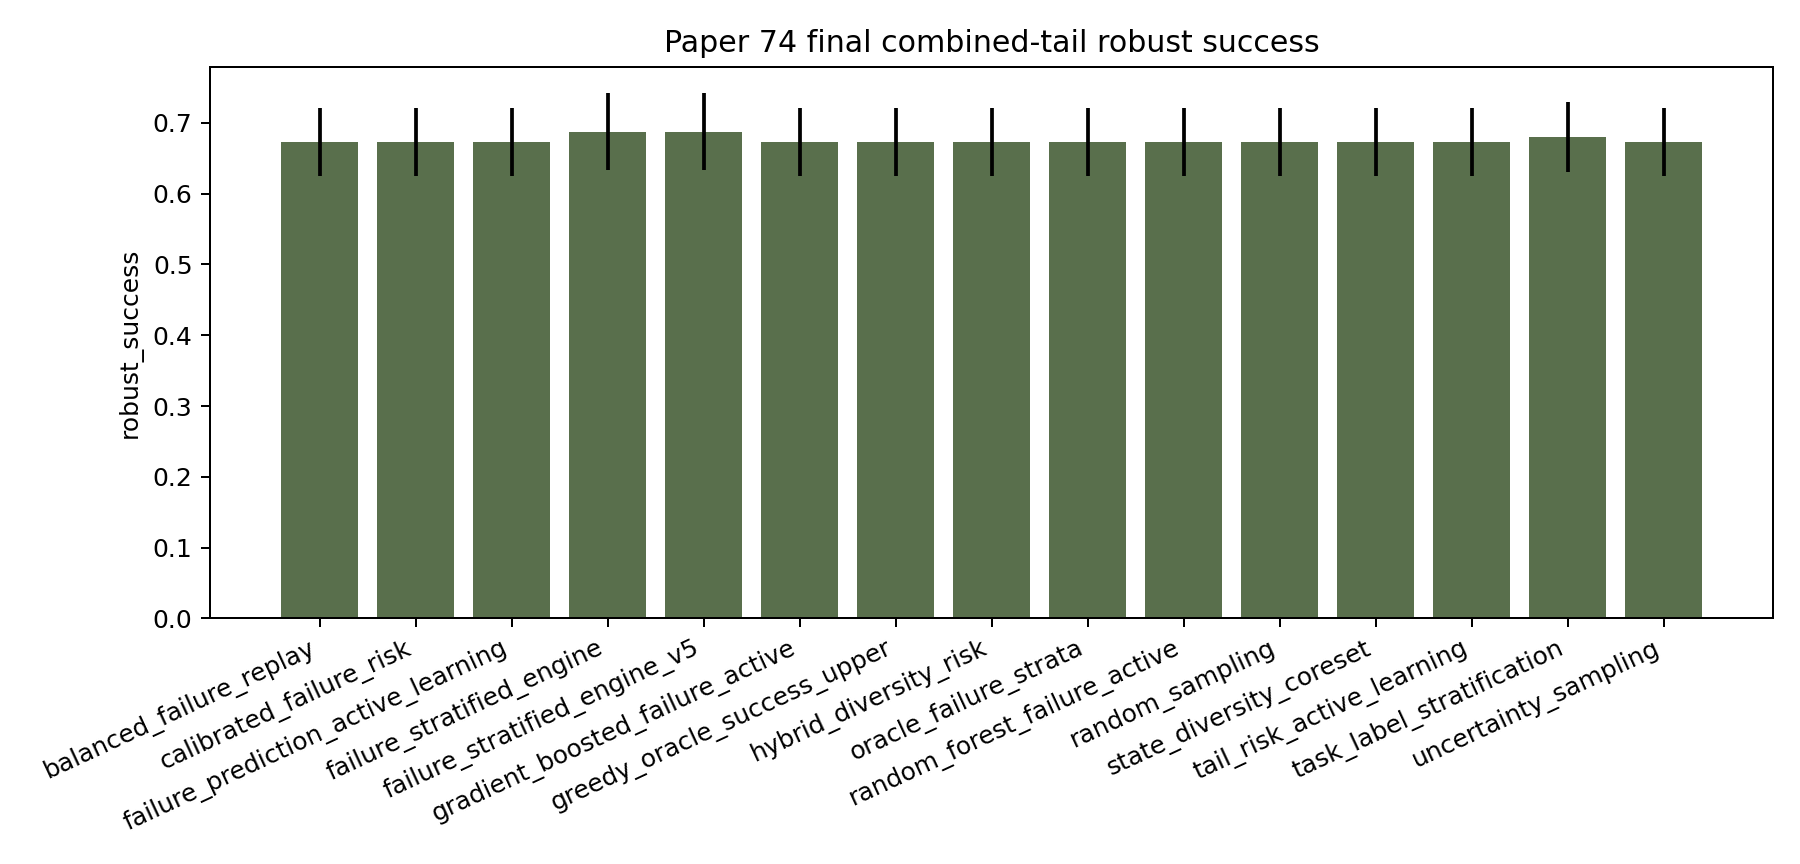
\includegraphics[width=0.95\linewidth]{../figures/failure_engine_final_success.png}
\caption{Combined-tail success by final method. The split alone would allow a tempting positive story, but the aggregate, fixed-risk, diagnostic, and ablation gates reject that story.}
\end{figure}

\section{Fixed-Risk Evaluation}
In a deployment-facing data engine, high success is less useful if the selector only succeeds by taking unbounded predicted risk. Table~\ref{tab:fixed010} counts abstentions as failures under a strict risk budget of 0.10. The proposed v5 method is not best; \texttt{rf-active} and \texttt{tail-risk} have higher hard-regime fixed-risk success.

\scriptsize
\setlength{\tabcolsep}{2pt}
\begin{center}
\refstepcounter{table}\label{tab:fixed010}\textbf{Table \thetable: Fixed-risk hard-regime success at budget 0.10. Abstentions count as failures; high coverage is useful only if selected actions remain successful.}\\[0.4ex]
\begin{tabular}{lcccc}
\toprule
Method & Success@0.10 & Coverage & Safety & Tail \\
\midrule
\texttt{rf-active} & $0.042 \pm 0.022$ & 0.064 & 0.014 & 0.022 \\
\texttt{tail-risk} & $0.042 \pm 0.019$ & 0.062 & 0.013 & 0.021 \\
\texttt{hybrid} & $0.032 \pm 0.016$ & 0.047 & 0.010 & 0.015 \\
\texttt{cal-risk} & $0.028 \pm 0.017$ & 0.047 & 0.011 & 0.019 \\
\texttt{fail-active} & $0.028 \pm 0.017$ & 0.049 & 0.013 & 0.021 \\
\texttt{uncertainty} & $0.028 \pm 0.015$ & 0.050 & 0.014 & 0.022 \\
\texttt{hgb-active} & $0.026 \pm 0.017$ & 0.043 & 0.010 & 0.017 \\
\texttt{replay} & $0.022 \pm 0.017$ & 0.042 & 0.013 & 0.019 \\
\texttt{random} & $0.022 \pm 0.015$ & 0.039 & 0.010 & 0.017 \\
\texttt{fs-v5} & $0.021 \pm 0.016$ & 0.037 & 0.013 & 0.017 \\
\texttt{task-label} & $0.018 \pm 0.012$ & 0.033 & 0.007 & 0.015 \\
\texttt{fs-v4} & $0.013 \pm 0.013$ & 0.025 & 0.007 & 0.013 \\
\texttt{oracle-strata} & $0.003 \pm 0.005$ & 0.004 & 0.001 & 0.001 \\
\texttt{oracle-success} & $0.001 \pm 0.003$ & 0.003 & 0.001 & 0.001 \\
\texttt{coreset} & $0.001 \pm 0.003$ & 0.006 & 0.003 & 0.004 \\
\bottomrule
\end{tabular}
\end{center}
\normalsize

\section{Combined-Tail Split}
Table~\ref{tab:combined} is the split most favorable to the proposed method: \texttt{fs-v5} ties \texttt{fs-v4} at 0.688 success and is above many non-oracle baselines on success. The gate still fails because the rare-recall and macro-F1 diagnostics are not better than \texttt{task-label}, and the broader hard-regime aggregate trails \texttt{replay}.

\scriptsize
\setlength{\tabcolsep}{2pt}
\begin{center}
\refstepcounter{table}\label{tab:combined}\textbf{Table \thetable: Combined-tail split. This split alone would make v5 look somewhat better on success, but the diagnostic and aggregate gates prevent overclaiming.}\\[0.4ex]
\begin{tabular}{lccccc}
\toprule
Method & Success & Macro F1 & Rare recall & Tail & Safety \\
\midrule
\texttt{fs-v4} & $0.688 \pm 0.054$ & 0.337 & 0.628 & 0.312 & 0.201 \\
\texttt{fs-v5} & $0.688 \pm 0.054$ & 0.337 & 0.604 & 0.312 & 0.201 \\
\texttt{task-label} & $0.681 \pm 0.049$ & 0.343 & 0.630 & 0.319 & 0.188 \\
\texttt{replay} & $0.674 \pm 0.048$ & 0.339 & 0.614 & 0.326 & 0.201 \\
\texttt{cal-risk} & $0.674 \pm 0.048$ & 0.345 & 0.600 & 0.326 & 0.201 \\
\texttt{fail-active} & $0.674 \pm 0.048$ & 0.345 & 0.602 & 0.326 & 0.201 \\
\texttt{hgb-active} & $0.674 \pm 0.048$ & 0.338 & 0.603 & 0.326 & 0.201 \\
\texttt{oracle-success} & $0.674 \pm 0.048$ & 0.333 & 0.647 & 0.326 & 0.201 \\
\texttt{hybrid} & $0.674 \pm 0.048$ & 0.332 & 0.605 & 0.326 & 0.201 \\
\texttt{oracle-strata} & $0.674 \pm 0.048$ & 0.333 & 0.637 & 0.326 & 0.201 \\
\texttt{rf-active} & $0.674 \pm 0.048$ & 0.347 & 0.610 & 0.326 & 0.201 \\
\texttt{random} & $0.674 \pm 0.048$ & 0.342 & 0.631 & 0.326 & 0.201 \\
\texttt{coreset} & $0.674 \pm 0.048$ & 0.330 & 0.618 & 0.326 & 0.194 \\
\texttt{tail-risk} & $0.674 \pm 0.048$ & 0.335 & 0.600 & 0.326 & 0.201 \\
\texttt{uncertainty} & $0.674 \pm 0.048$ & 0.349 & 0.618 & 0.326 & 0.201 \\
\bottomrule
\end{tabular}
\end{center}
\normalsize

\section{Ablation Results}
Table~\ref{tab:ablation} is the most damaging mechanistic evidence. Removing calibration, diversity, mechanism deficit, rare weighting, tail risk, trace features, or reverting to the old score matches or beats full v5 within the frozen tolerance. That means the claimed v5 components are not identified as necessary.

\scriptsize
\setlength{\tabcolsep}{2pt}
\begin{center}
\refstepcounter{table}\label{tab:ablation}\textbf{Table \thetable: V5 ablations on combined-tail stress. The full method must not be matched by removing claimed core components.}\\[0.4ex]
\begin{tabular}{lccccc}
\toprule
Ablation & Success & Macro F1 & Rare recall & Tail & Safety \\
\midrule
\texttt{no-mech-deficit} & $0.694 \pm 0.082$ & 0.325 & 0.591 & 0.312 & 0.139 \\
\texttt{no-rare} & $0.694 \pm 0.082$ & 0.320 & 0.576 & 0.312 & 0.139 \\
\texttt{no-tail} & $0.694 \pm 0.082$ & 0.339 & 0.590 & 0.312 & 0.139 \\
\texttt{no-trace} & $0.694 \pm 0.082$ & 0.321 & 0.580 & 0.312 & 0.139 \\
\texttt{old-score} & $0.694 \pm 0.082$ & 0.327 & 0.577 & 0.312 & 0.139 \\
\texttt{full-v5} & $0.667 \pm 0.118$ & 0.321 & 0.574 & 0.333 & 0.153 \\
\texttt{no-cal} & $0.667 \pm 0.118$ & 0.322 & 0.574 & 0.333 & 0.153 \\
\texttt{no-diversity} & $0.667 \pm 0.118$ & 0.321 & 0.574 & 0.333 & 0.153 \\
\bottomrule
\end{tabular}
\end{center}
\normalsize

\begin{figure}[t]
\centering
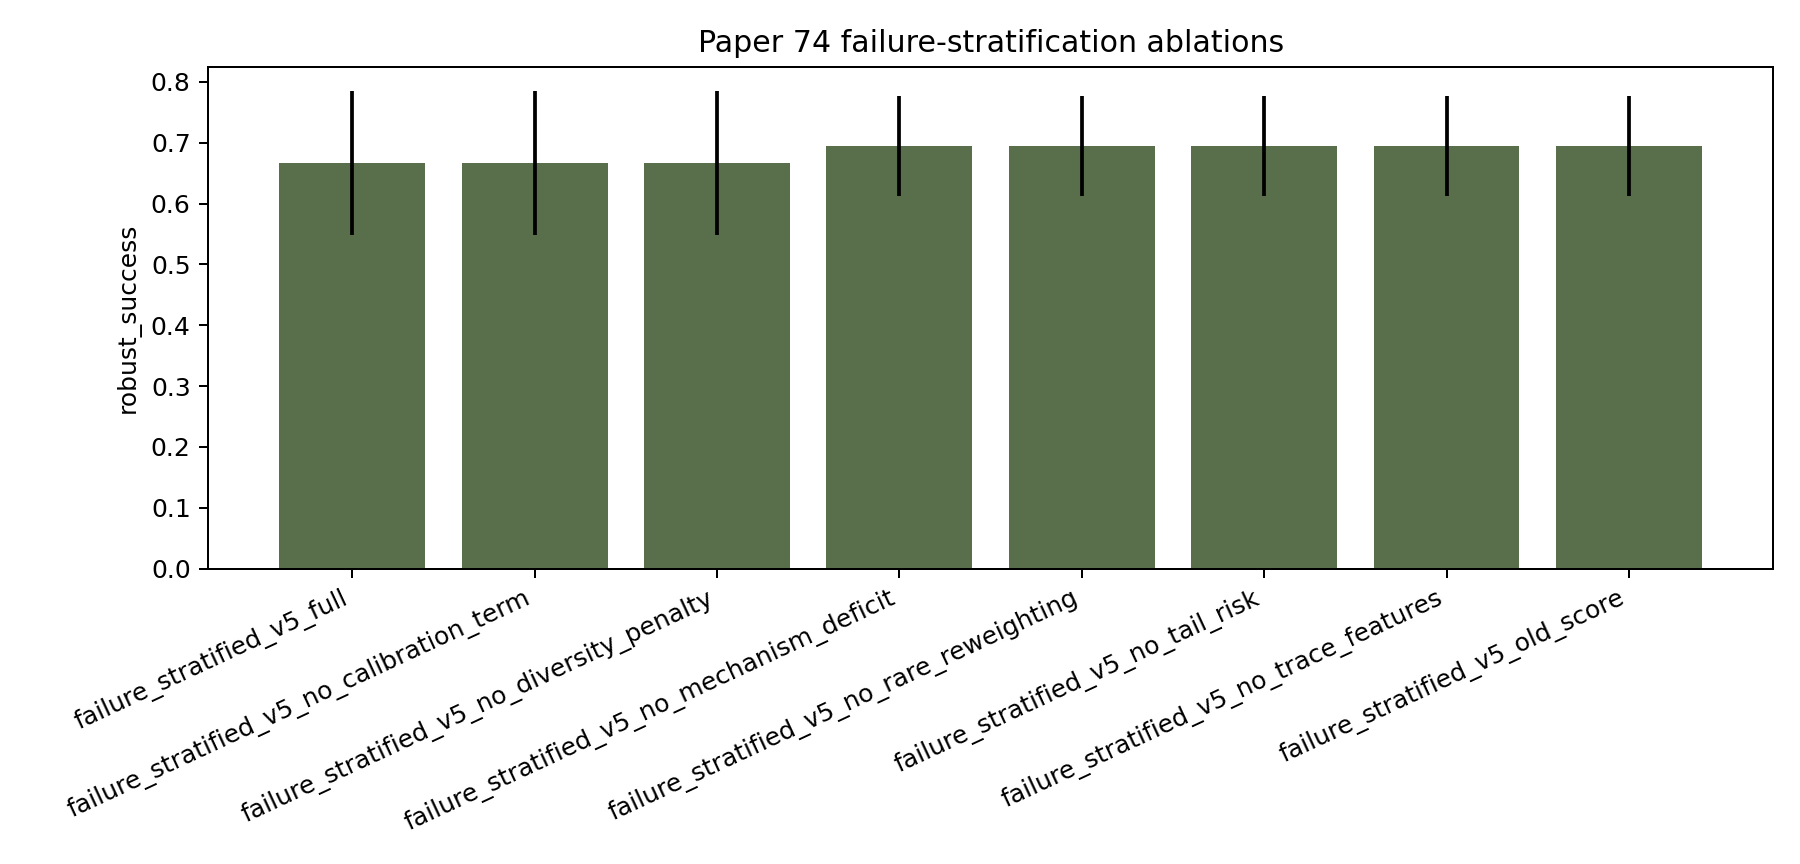
\includegraphics[width=0.95\linewidth]{../figures/failure_engine_ablation_success.png}
\caption{Ablation success on combined-tail stress. Full v5 is not protected by its claimed components.}
\end{figure}

\section{Data Efficiency}
Acquisition papers should not only report the final point after a large budget. We therefore also inspect round-by-round performance on the combined-tail split. Figure~\ref{fig:roundsuccess} and Figure~\ref{fig:roundrare} show that the proposed method does not produce a clean data-efficiency separation: rare recall moves, but downstream success remains largely tied with strong non-oracle selectors. The full per-round table appears in Appendix~\ref{sec:roundappendix}.

\begin{figure}[t]
\centering
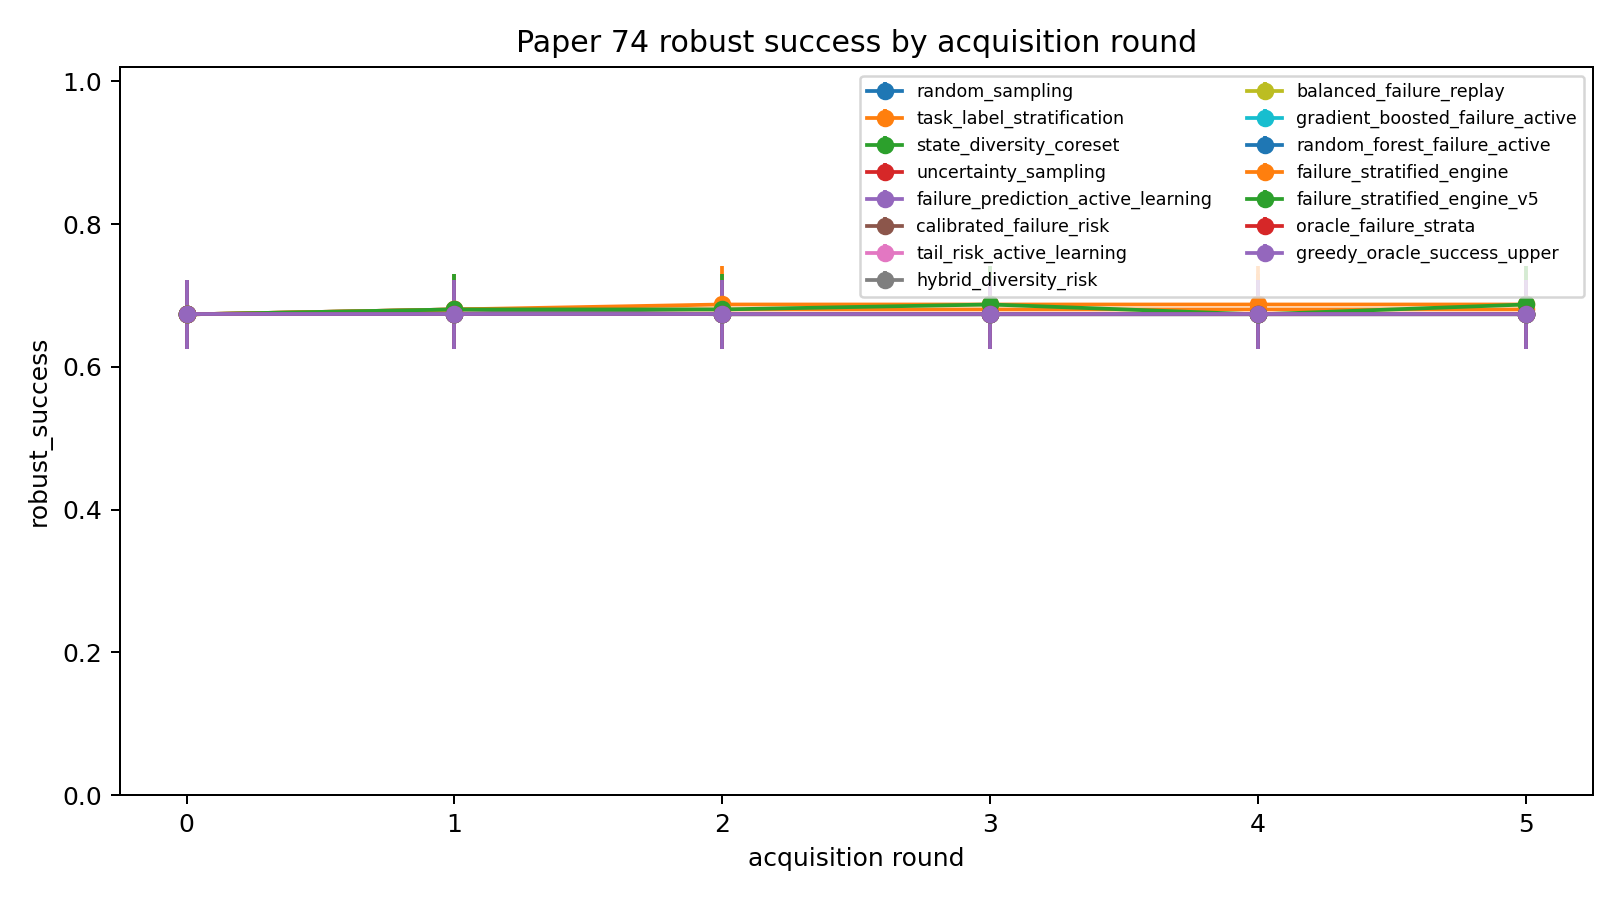
\includegraphics[width=0.92\linewidth]{../figures/failure_engine_success_by_round.png}
\caption{Combined-tail robust success by acquisition round.}
\label{fig:roundsuccess}
\end{figure}

\begin{figure}[t]
\centering
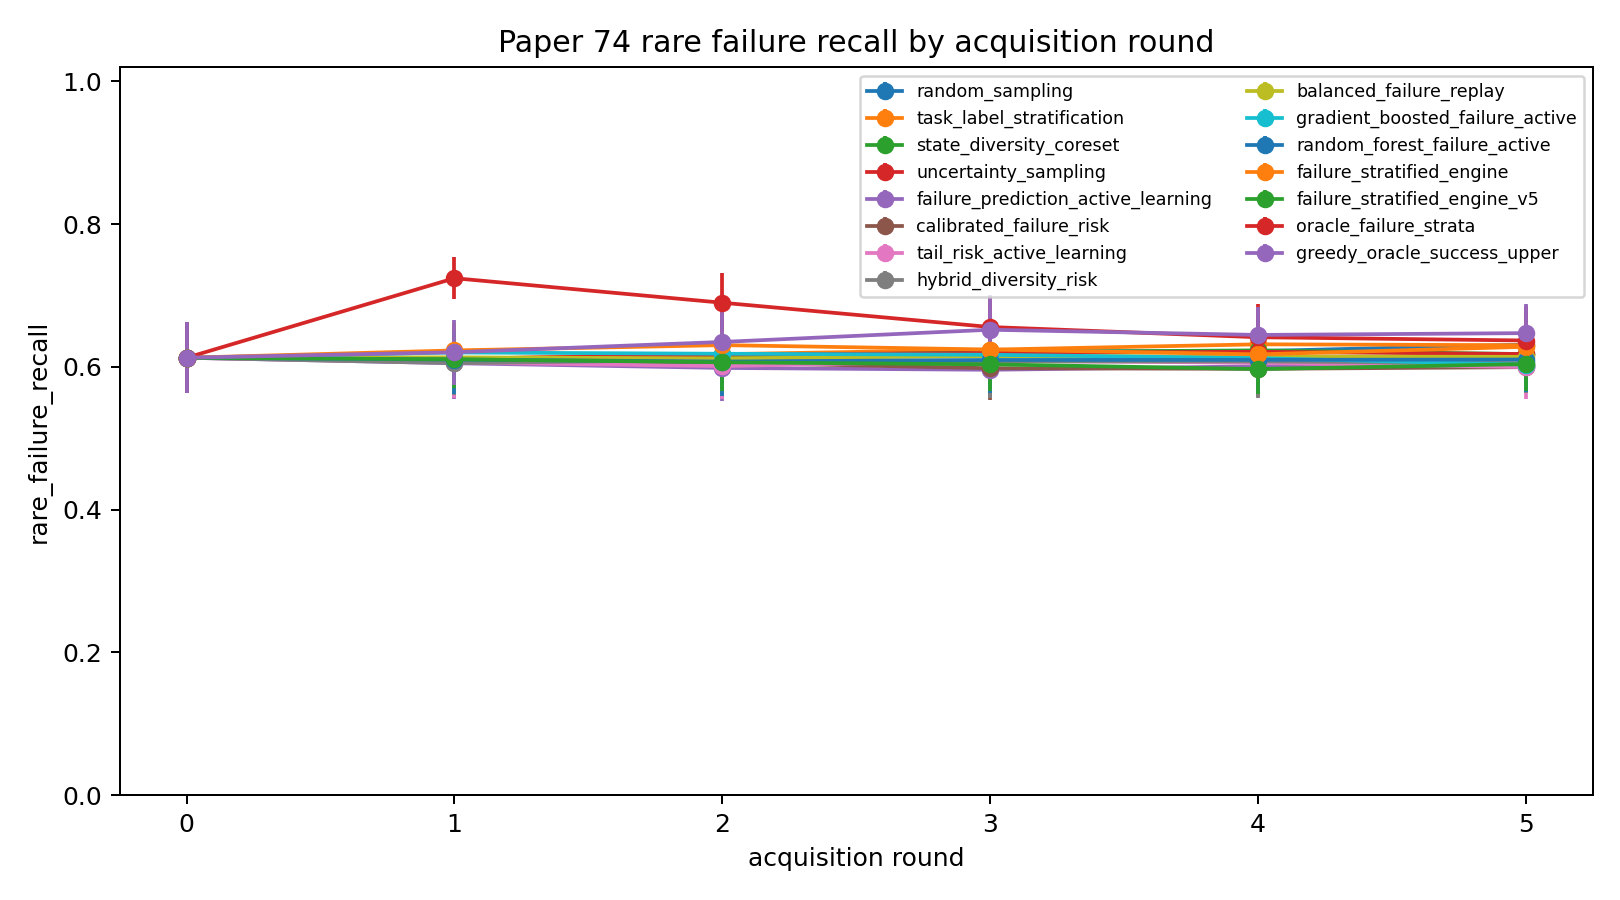
\includegraphics[width=0.92\linewidth]{../figures/failure_engine_rare_recall_by_round.png}
\caption{Combined-tail rare failure recall by acquisition round.}
\label{fig:roundrare}
\end{figure}

\section{Stress Sweep}
The stress sweep tests whether the proposed engine collapses later than strong baselines as severity increases. Table~\ref{tab:maxstress} reports the maximum-stress endpoint. The proposed method is not meaningfully ahead of the strongest non-oracle method.

\scriptsize
\setlength{\tabcolsep}{2pt}
\begin{center}
\refstepcounter{table}\label{tab:maxstress}\textbf{Table \thetable: Maximum-stress comparison at severity 1.00.}\\[0.4ex]
\begin{tabular}{lccccc}
\toprule
Method & Success & Macro F1 & Rare recall & Tail & Safety \\
\midrule
\texttt{cal-risk} & $0.013 \pm 0.025$ & 0.494 & 0.807 & 0.988 & 0.713 \\
\texttt{fail-active} & $0.013 \pm 0.025$ & 0.494 & 0.807 & 0.988 & 0.713 \\
\texttt{fs-v4} & $0.013 \pm 0.025$ & 0.497 & 0.841 & 0.988 & 0.713 \\
\texttt{fs-v5} & $0.013 \pm 0.025$ & 0.494 & 0.831 & 0.988 & 0.713 \\
\texttt{hybrid} & $0.013 \pm 0.025$ & 0.487 & 0.771 & 0.988 & 0.713 \\
\texttt{oracle-strata} & $0.013 \pm 0.025$ & 0.503 & 0.860 & 0.988 & 0.713 \\
\texttt{uncertainty} & $0.013 \pm 0.025$ & 0.500 & 0.838 & 0.988 & 0.713 \\
\bottomrule
\end{tabular}
\end{center}
\normalsize

\begin{figure}[t]
\centering
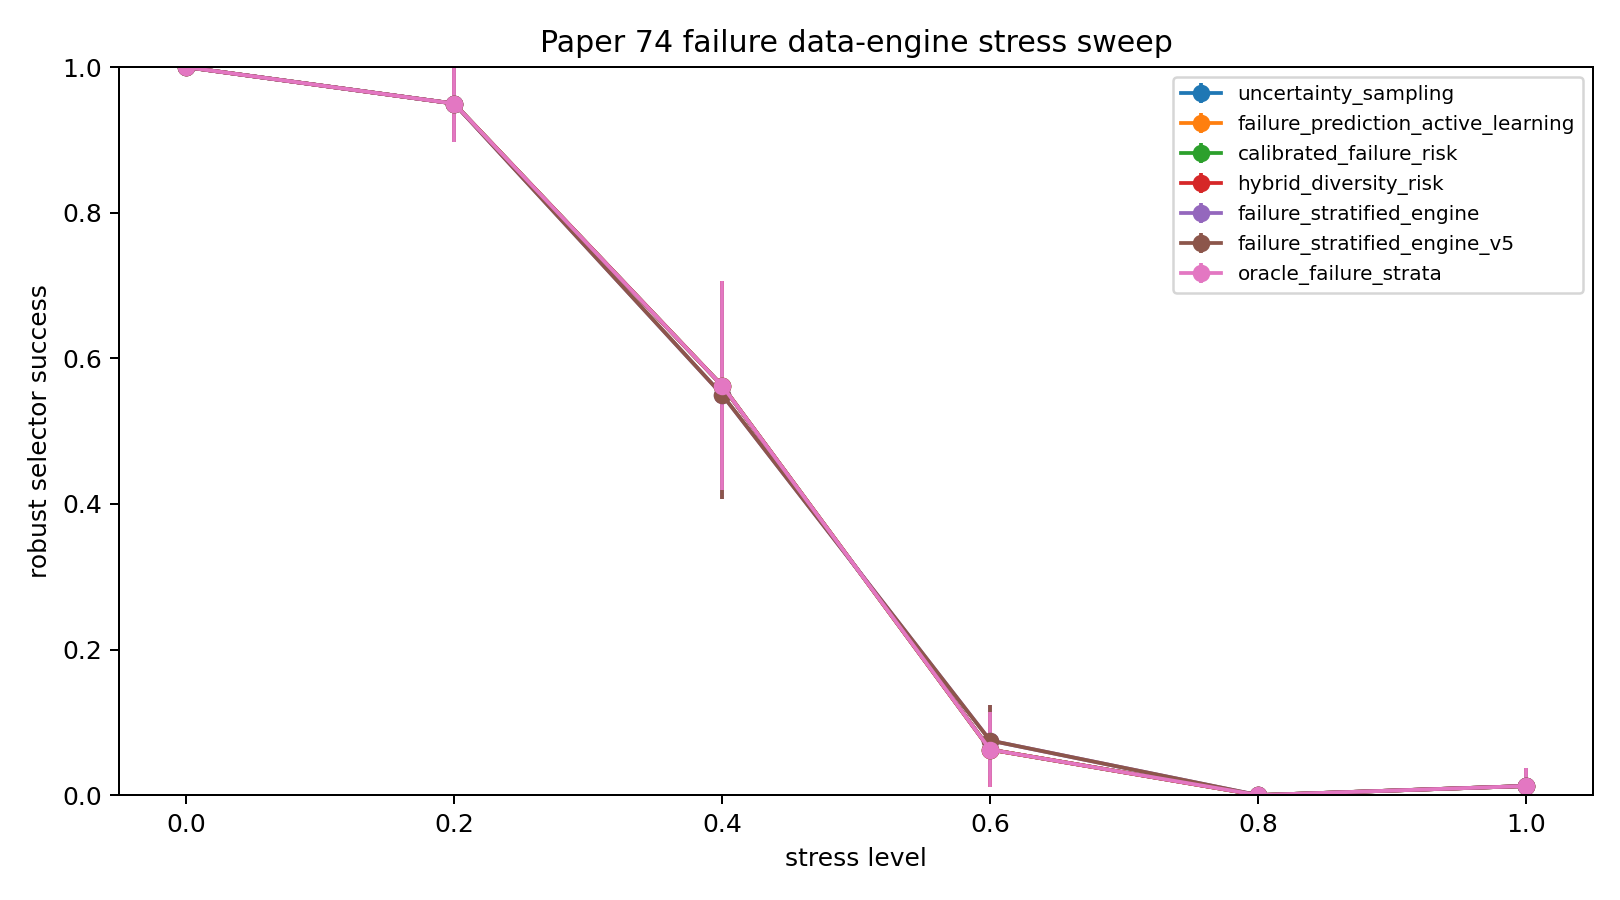
\includegraphics[width=0.95\linewidth]{../figures/failure_engine_stress_sweep.png}
\caption{Stress sweep over combined-tail severity. The proposed method does not establish a robust maximum-stress advantage.}
\end{figure}

\section{Negative Cases}
Negative cases show the selector-level failure mode: the data engine may acquire or predict rare mechanisms, yet the trained robust selector still chooses a tail-risk policy. This is not a formatting problem; it is a scientific failure of the central mechanism-to-control link.

\tiny
\setlength{\tabcolsep}{2pt}
\begin{center}
\refstepcounter{table}\label{tab:negcases}\textbf{Table \thetable: Representative negative cases mined from the frozen v5 run.}\\[0.4ex]
\begin{tabular}{p{0.035\linewidth}p{0.13\linewidth}p{0.12\linewidth}p{0.23\linewidth}p{0.055\linewidth}p{0.045\linewidth}p{0.21\linewidth}}
\toprule
Seed & Scenario & Policy & Failures & Progress & Safety & Lesson \\
\midrule
0 & cts\_0\_684 & \texttt{fric-probe} & slip, missed\_contact, sensor\_dropout & 1.018 & 0.000 & coverage pressure did not convert to safe selection \\
0 & cts\_0\_686 & \texttt{fric-probe} & jam, fixture\_collision, sensor\_dropout, timeout & 0.282 & 1.000 & coverage pressure did not convert to safe selection \\
0 & cts\_0\_689 & \texttt{fric-probe} & missed\_contact, timeout & 0.000 & 0.000 & coverage pressure did not convert to safe selection \\
0 & cts\_0\_690 & \texttt{fric-probe} & jam, fixture\_collision, timeout & 0.312 & 1.000 & coverage pressure did not convert to safe selection \\
0 & cts\_0\_692 & \texttt{fric-probe} & jam, fixture\_collision, timeout & 0.270 & 1.000 & coverage pressure did not convert to safe selection \\
0 & cts\_0\_694 & \texttt{fric-probe} & jam, fixture\_collision, sensor\_dropout, timeout & 0.291 & 1.000 & coverage pressure did not convert to safe selection \\
0 & cts\_0\_695 & \texttt{fric-probe} & jam, fixture\_collision, sensor\_dropout, timeout & 0.258 & 1.000 & coverage pressure did not convert to safe selection \\
0 & cts\_0\_698 & \texttt{fric-probe} & slip, sensor\_dropout, timeout & 0.717 & 0.000 & coverage pressure did not convert to safe selection \\
1 & cts\_1\_688 & \texttt{fric-probe} & jam, fixture\_collision, sensor\_dropout, timeout & 0.278 & 1.000 & coverage pressure did not convert to safe selection \\
1 & cts\_1\_692 & \texttt{fric-probe} & jam, sensor\_dropout, timeout & 0.000 & 0.000 & coverage pressure did not convert to safe selection \\
1 & cts\_1\_696 & \texttt{fric-probe} & jam, fixture\_collision, timeout & 0.130 & 1.000 & coverage pressure did not convert to safe selection \\
1 & cts\_1\_699 & \texttt{fric-probe} & missed\_contact, sensor\_dropout, timeout & 0.120 & 0.000 & coverage pressure did not convert to safe selection \\
\bottomrule
\end{tabular}
\end{center}
\normalsize

\section{Limitations}
This is not a hardware paper. It has no real-robot validation, no videos, no external public benchmark run, and no large policy checkpoint. Those missing pieces would keep even a positive result at \texttt{STRONG\_REVISE} rather than main-conference ready. Because the central frozen gates fail, the honest decision is lower: \texttt{KILL\_ARCHIVE}.

\section{Conclusion}
The expanded v5 audit gives Paper 74 every reasonable local chance: more splits, more baselines, a stronger proposed method, hard-regime aggregates, fixed-risk selection, ablations, stress sweeps, and a full appendix. The result remains negative. Failure stratification is not enough unless mechanism coverage changes the action selector's downstream decisions under the hard regimes reviewers will care about.

\appendix
\section{Complete Main Metrics}
\tiny
\setlength{\tabcolsep}{2pt}
\begin{center}
\refstepcounter{table}\label{tab:allmetrics}\textbf{Table \thetable: All method/split summary rows from the frozen v5 run.}\\[0.4ex]
\begin{tabular}{llcccccc}
\toprule
Method & Split & Success & Macro F1 & Rare recall & Tail & Calib & Safety \\
\midrule
\texttt{replay} & \texttt{actuator} & $1.000 \pm 0.000$ & 0.057 & 0.000 & 0.000 & 0.093 & 0.000 \\
\texttt{replay} & \texttt{nominal} & $1.000 \pm 0.000$ & 0.000 & 0.000 & 0.000 & 0.040 & 0.000 \\
\texttt{cal-risk} & \texttt{actuator} & $1.000 \pm 0.000$ & 0.006 & 0.000 & 0.000 & 0.079 & 0.000 \\
\texttt{cal-risk} & \texttt{nominal} & $1.000 \pm 0.000$ & 0.000 & 0.000 & 0.000 & 0.030 & 0.000 \\
\texttt{fail-active} & \texttt{actuator} & $1.000 \pm 0.000$ & 0.003 & 0.000 & 0.000 & 0.075 & 0.000 \\
\texttt{fail-active} & \texttt{nominal} & $1.000 \pm 0.000$ & 0.000 & 0.000 & 0.000 & 0.030 & 0.000 \\
\texttt{fs-v4} & \texttt{nominal} & $1.000 \pm 0.000$ & 0.000 & 0.000 & 0.000 & 0.030 & 0.000 \\
\texttt{fs-v5} & \texttt{nominal} & $1.000 \pm 0.000$ & 0.000 & 0.000 & 0.000 & 0.040 & 0.000 \\
\texttt{hgb-active} & \texttt{actuator} & $1.000 \pm 0.000$ & 0.062 & 0.000 & 0.000 & 0.095 & 0.000 \\
\texttt{hgb-active} & \texttt{nominal} & $1.000 \pm 0.000$ & 0.000 & 0.000 & 0.000 & 0.040 & 0.000 \\
\texttt{oracle-success} & \texttt{actuator} & $1.000 \pm 0.000$ & 0.034 & 0.000 & 0.000 & 0.083 & 0.000 \\
\texttt{oracle-success} & \texttt{nominal} & $1.000 \pm 0.000$ & 0.000 & 0.000 & 0.000 & 0.041 & 0.000 \\
\texttt{hybrid} & \texttt{actuator} & $1.000 \pm 0.000$ & 0.054 & 0.000 & 0.000 & 0.088 & 0.000 \\
\texttt{hybrid} & \texttt{nominal} & $1.000 \pm 0.000$ & 0.000 & 0.000 & 0.000 & 0.044 & 0.000 \\
\texttt{oracle-strata} & \texttt{actuator} & $1.000 \pm 0.000$ & 0.043 & 0.000 & 0.000 & 0.090 & 0.000 \\
\texttt{oracle-strata} & \texttt{nominal} & $1.000 \pm 0.000$ & 0.005 & 0.000 & 0.000 & 0.048 & 0.000 \\
\texttt{rf-active} & \texttt{actuator} & $1.000 \pm 0.000$ & 0.056 & 0.000 & 0.000 & 0.088 & 0.000 \\
\texttt{rf-active} & \texttt{nominal} & $1.000 \pm 0.000$ & 0.000 & 0.000 & 0.000 & 0.041 & 0.000 \\
\texttt{random} & \texttt{actuator} & $1.000 \pm 0.000$ & 0.046 & 0.000 & 0.000 & 0.092 & 0.000 \\
\texttt{random} & \texttt{nominal} & $1.000 \pm 0.000$ & 0.000 & 0.000 & 0.000 & 0.041 & 0.000 \\
\texttt{coreset} & \texttt{actuator} & $1.000 \pm 0.000$ & 0.055 & 0.000 & 0.000 & 0.096 & 0.000 \\
\texttt{coreset} & \texttt{nominal} & $1.000 \pm 0.000$ & 0.000 & 0.000 & 0.000 & 0.045 & 0.000 \\
\texttt{tail-risk} & \texttt{actuator} & $1.000 \pm 0.000$ & 0.050 & 0.000 & 0.000 & 0.092 & 0.000 \\
\texttt{tail-risk} & \texttt{nominal} & $1.000 \pm 0.000$ & 0.000 & 0.000 & 0.000 & 0.036 & 0.000 \\
\texttt{task-label} & \texttt{nominal} & $1.000 \pm 0.000$ & 0.000 & 0.000 & 0.000 & 0.038 & 0.000 \\
\texttt{uncertainty} & \texttt{actuator} & $1.000 \pm 0.000$ & 0.061 & 0.000 & 0.000 & 0.092 & 0.000 \\
\texttt{uncertainty} & \texttt{nominal} & $1.000 \pm 0.000$ & 0.000 & 0.000 & 0.000 & 0.041 & 0.000 \\
\texttt{fs-v4} & \texttt{actuator} & $0.993 \pm 0.014$ & 0.053 & 0.000 & 0.007 & 0.085 & 0.000 \\
\texttt{fs-v5} & \texttt{actuator} & $0.993 \pm 0.014$ & 0.060 & 0.000 & 0.007 & 0.090 & 0.000 \\
\texttt{task-label} & \texttt{actuator} & $0.986 \pm 0.027$ & 0.062 & 0.000 & 0.014 & 0.088 & 0.000 \\
\texttt{replay} & \texttt{rare-slip} & $0.965 \pm 0.029$ & 0.165 & 0.093 & 0.035 & 0.074 & 0.007 \\
\texttt{cal-risk} & \texttt{rare-slip} & $0.965 \pm 0.029$ & 0.118 & 0.101 & 0.035 & 0.090 & 0.007 \\
\texttt{fail-active} & \texttt{rare-slip} & $0.965 \pm 0.029$ & 0.117 & 0.101 & 0.035 & 0.088 & 0.007 \\
\texttt{fs-v4} & \texttt{rare-slip} & $0.965 \pm 0.029$ & 0.167 & 0.094 & 0.035 & 0.089 & 0.007 \\
\bottomrule
\end{tabular}
\end{center}
\begin{center}
\textbf{Table \ref{tab:allmetrics} continued}\\[0.4ex]
\begin{tabular}{llcccccc}
\toprule
Method & Split & Success & Macro F1 & Rare recall & Tail & Calib & Safety \\
\midrule
\texttt{fs-v5} & \texttt{rare-slip} & $0.965 \pm 0.029$ & 0.178 & 0.138 & 0.035 & 0.081 & 0.007 \\
\texttt{hgb-active} & \texttt{rare-slip} & $0.965 \pm 0.029$ & 0.166 & 0.082 & 0.035 & 0.080 & 0.007 \\
\texttt{oracle-success} & \texttt{rare-slip} & $0.965 \pm 0.029$ & 0.159 & 0.117 & 0.035 & 0.098 & 0.007 \\
\texttt{hybrid} & \texttt{rare-slip} & $0.965 \pm 0.029$ & 0.169 & 0.122 & 0.035 & 0.083 & 0.007 \\
\texttt{oracle-strata} & \texttt{rare-slip} & $0.965 \pm 0.029$ & 0.190 & 0.147 & 0.035 & 0.097 & 0.007 \\
\texttt{rf-active} & \texttt{rare-slip} & $0.965 \pm 0.029$ & 0.157 & 0.034 & 0.035 & 0.085 & 0.007 \\
\texttt{random} & \texttt{rare-slip} & $0.965 \pm 0.029$ & 0.170 & 0.076 & 0.035 & 0.078 & 0.007 \\
\texttt{tail-risk} & \texttt{rare-slip} & $0.965 \pm 0.029$ & 0.156 & 0.095 & 0.035 & 0.082 & 0.007 \\
\texttt{task-label} & \texttt{rare-slip} & $0.965 \pm 0.029$ & 0.176 & 0.090 & 0.035 & 0.088 & 0.007 \\
\texttt{uncertainty} & \texttt{rare-slip} & $0.965 \pm 0.029$ & 0.188 & 0.113 & 0.035 & 0.083 & 0.007 \\
\texttt{coreset} & \texttt{rare-slip} & $0.958 \pm 0.034$ & 0.174 & 0.116 & 0.042 & 0.086 & 0.014 \\
\texttt{task-label} & \texttt{sensor-actuator} & $0.743 \pm 0.050$ & 0.265 & 0.474 & 0.257 & 0.161 & 0.139 \\
\texttt{replay} & \texttt{sensor-actuator} & $0.736 \pm 0.053$ & 0.259 & 0.420 & 0.264 & 0.164 & 0.167 \\
\texttt{cal-risk} & \texttt{sensor-actuator} & $0.736 \pm 0.053$ & 0.250 & 0.433 & 0.264 & 0.157 & 0.167 \\
\texttt{fail-active} & \texttt{sensor-actuator} & $0.736 \pm 0.053$ & 0.247 & 0.431 & 0.264 & 0.164 & 0.167 \\
\texttt{hgb-active} & \texttt{sensor-actuator} & $0.736 \pm 0.053$ & 0.264 & 0.454 & 0.264 & 0.161 & 0.167 \\
\texttt{oracle-success} & \texttt{sensor-actuator} & $0.736 \pm 0.053$ & 0.288 & 0.657 & 0.264 & 0.171 & 0.167 \\
\texttt{hybrid} & \texttt{sensor-actuator} & $0.736 \pm 0.053$ & 0.273 & 0.449 & 0.264 & 0.146 & 0.167 \\
\texttt{oracle-strata} & \texttt{sensor-actuator} & $0.736 \pm 0.053$ & 0.281 & 0.635 & 0.264 & 0.184 & 0.167 \\
\texttt{rf-active} & \texttt{sensor-actuator} & $0.736 \pm 0.053$ & 0.240 & 0.401 & 0.264 & 0.170 & 0.167 \\
\texttt{random} & \texttt{sensor-actuator} & $0.736 \pm 0.053$ & 0.261 & 0.469 & 0.264 & 0.161 & 0.167 \\
\texttt{tail-risk} & \texttt{sensor-actuator} & $0.736 \pm 0.053$ & 0.281 & 0.460 & 0.264 & 0.157 & 0.167 \\
\texttt{uncertainty} & \texttt{sensor-actuator} & $0.736 \pm 0.053$ & 0.254 & 0.408 & 0.264 & 0.175 & 0.167 \\
\texttt{fs-v4} & \texttt{sensor-actuator} & $0.729 \pm 0.060$ & 0.265 & 0.517 & 0.271 & 0.194 & 0.181 \\
\texttt{fs-v5} & \texttt{sensor-actuator} & $0.729 \pm 0.060$ & 0.254 & 0.391 & 0.271 & 0.159 & 0.181 \\
\texttt{coreset} & \texttt{sensor-actuator} & $0.729 \pm 0.043$ & 0.267 & 0.536 & 0.271 & 0.141 & 0.167 \\
\texttt{fs-v4} & \texttt{combined} & $0.688 \pm 0.054$ & 0.337 & 0.628 & 0.312 & 0.220 & 0.201 \\
\texttt{fs-v5} & \texttt{combined} & $0.688 \pm 0.054$ & 0.337 & 0.604 & 0.312 & 0.151 & 0.201 \\
\texttt{task-label} & \texttt{combined} & $0.681 \pm 0.049$ & 0.343 & 0.630 & 0.319 & 0.152 & 0.188 \\
\texttt{replay} & \texttt{combined} & $0.674 \pm 0.048$ & 0.339 & 0.614 & 0.326 & 0.156 & 0.201 \\
\texttt{cal-risk} & \texttt{combined} & $0.674 \pm 0.048$ & 0.345 & 0.600 & 0.326 & 0.121 & 0.201 \\
\texttt{fail-active} & \texttt{combined} & $0.674 \pm 0.048$ & 0.345 & 0.602 & 0.326 & 0.117 & 0.201 \\
\texttt{hgb-active} & \texttt{combined} & $0.674 \pm 0.048$ & 0.338 & 0.603 & 0.326 & 0.155 & 0.201 \\
\texttt{oracle-success} & \texttt{combined} & $0.674 \pm 0.048$ & 0.333 & 0.647 & 0.326 & 0.178 & 0.201 \\
\bottomrule
\end{tabular}
\end{center}
\begin{center}
\textbf{Table \ref{tab:allmetrics} continued}\\[0.4ex]
\begin{tabular}{llcccccc}
\toprule
Method & Split & Success & Macro F1 & Rare recall & Tail & Calib & Safety \\
\midrule
\texttt{hybrid} & \texttt{combined} & $0.674 \pm 0.048$ & 0.332 & 0.605 & 0.326 & 0.138 & 0.201 \\
\texttt{oracle-strata} & \texttt{combined} & $0.674 \pm 0.048$ & 0.333 & 0.637 & 0.326 & 0.171 & 0.201 \\
\texttt{rf-active} & \texttt{combined} & $0.674 \pm 0.048$ & 0.347 & 0.610 & 0.326 & 0.151 & 0.201 \\
\texttt{random} & \texttt{combined} & $0.674 \pm 0.048$ & 0.342 & 0.631 & 0.326 & 0.157 & 0.201 \\
\texttt{coreset} & \texttt{combined} & $0.674 \pm 0.048$ & 0.330 & 0.618 & 0.326 & 0.143 & 0.194 \\
\texttt{tail-risk} & \texttt{combined} & $0.674 \pm 0.048$ & 0.335 & 0.600 & 0.326 & 0.139 & 0.201 \\
\texttt{uncertainty} & \texttt{combined} & $0.674 \pm 0.048$ & 0.349 & 0.618 & 0.326 & 0.140 & 0.201 \\
\texttt{replay} & \texttt{rare-combo} & $0.486 \pm 0.138$ & 0.354 & 0.554 & 0.514 & 0.111 & 0.007 \\
\texttt{cal-risk} & \texttt{rare-combo} & $0.486 \pm 0.138$ & 0.328 & 0.437 & 0.514 & 0.117 & 0.007 \\
\texttt{fail-active} & \texttt{rare-combo} & $0.486 \pm 0.138$ & 0.326 & 0.437 & 0.514 & 0.120 & 0.007 \\
\texttt{hgb-active} & \texttt{rare-combo} & $0.486 \pm 0.138$ & 0.356 & 0.549 & 0.514 & 0.111 & 0.007 \\
\texttt{oracle-success} & \texttt{rare-combo} & $0.486 \pm 0.138$ & 0.317 & 0.468 & 0.514 & 0.111 & 0.007 \\
\texttt{hybrid} & \texttt{rare-combo} & $0.486 \pm 0.138$ & 0.338 & 0.526 & 0.514 & 0.126 & 0.007 \\
\texttt{oracle-strata} & \texttt{rare-combo} & $0.486 \pm 0.138$ & 0.317 & 0.487 & 0.514 & 0.105 & 0.007 \\
\texttt{rf-active} & \texttt{rare-combo} & $0.486 \pm 0.138$ & 0.324 & 0.506 & 0.514 & 0.128 & 0.007 \\
\texttt{random} & \texttt{rare-combo} & $0.486 \pm 0.138$ & 0.345 & 0.541 & 0.514 & 0.101 & 0.007 \\
\texttt{tail-risk} & \texttt{rare-combo} & $0.486 \pm 0.138$ & 0.357 & 0.503 & 0.514 & 0.117 & 0.007 \\
\texttt{uncertainty} & \texttt{rare-combo} & $0.486 \pm 0.138$ & 0.339 & 0.522 & 0.514 & 0.093 & 0.007 \\
\texttt{fs-v4} & \texttt{rare-combo} & $0.465 \pm 0.128$ & 0.334 & 0.518 & 0.535 & 0.123 & 0.014 \\
\texttt{fs-v5} & \texttt{rare-combo} & $0.465 \pm 0.128$ & 0.338 & 0.568 & 0.535 & 0.115 & 0.014 \\
\texttt{task-label} & \texttt{rare-combo} & $0.465 \pm 0.128$ & 0.324 & 0.486 & 0.535 & 0.092 & 0.007 \\
\texttt{replay} & \texttt{ood-tail} & $0.458 \pm 0.136$ & 0.327 & 0.489 & 0.542 & 0.168 & 0.007 \\
\texttt{cal-risk} & \texttt{ood-tail} & $0.458 \pm 0.136$ & 0.316 & 0.407 & 0.542 & 0.182 & 0.007 \\
\texttt{fail-active} & \texttt{ood-tail} & $0.458 \pm 0.136$ & 0.315 & 0.414 & 0.542 & 0.184 & 0.007 \\
\texttt{hgb-active} & \texttt{ood-tail} & $0.458 \pm 0.136$ & 0.329 & 0.520 & 0.542 & 0.178 & 0.007 \\
\texttt{oracle-success} & \texttt{ood-tail} & $0.458 \pm 0.136$ & 0.314 & 0.503 & 0.542 & 0.175 & 0.007 \\
\texttt{hybrid} & \texttt{ood-tail} & $0.458 \pm 0.136$ & 0.333 & 0.486 & 0.542 & 0.159 & 0.007 \\
\texttt{oracle-strata} & \texttt{ood-tail} & $0.458 \pm 0.136$ & 0.309 & 0.477 & 0.542 & 0.182 & 0.007 \\
\texttt{rf-active} & \texttt{ood-tail} & $0.458 \pm 0.136$ & 0.322 & 0.526 & 0.542 & 0.185 & 0.007 \\
\texttt{random} & \texttt{ood-tail} & $0.458 \pm 0.136$ & 0.321 & 0.457 & 0.542 & 0.178 & 0.007 \\
\texttt{tail-risk} & \texttt{ood-tail} & $0.458 \pm 0.136$ & 0.324 & 0.431 & 0.542 & 0.179 & 0.007 \\
\texttt{uncertainty} & \texttt{ood-tail} & $0.458 \pm 0.136$ & 0.312 & 0.457 & 0.542 & 0.189 & 0.007 \\
\texttt{coreset} & \texttt{rare-combo} & $0.444 \pm 0.122$ & 0.322 & 0.488 & 0.556 & 0.114 & 0.007 \\
\texttt{coreset} & \texttt{ood-tail} & $0.444 \pm 0.146$ & 0.322 & 0.506 & 0.556 & 0.178 & 0.000 \\
\bottomrule
\end{tabular}
\end{center}
\begin{center}
\textbf{Table \ref{tab:allmetrics} continued}\\[0.4ex]
\begin{tabular}{llcccccc}
\toprule
Method & Split & Success & Macro F1 & Rare recall & Tail & Calib & Safety \\
\midrule
\texttt{fs-v4} & \texttt{ood-tail} & $0.431 \pm 0.130$ & 0.316 & 0.485 & 0.569 & 0.179 & 0.007 \\
\texttt{fs-v5} & \texttt{ood-tail} & $0.431 \pm 0.130$ & 0.323 & 0.484 & 0.569 & 0.168 & 0.007 \\
\texttt{task-label} & \texttt{ood-tail} & $0.424 \pm 0.132$ & 0.321 & 0.478 & 0.576 & 0.172 & 0.007 \\
\texttt{replay} & \texttt{fixture-shift} & $0.021 \pm 0.020$ & 0.341 & 0.400 & 0.979 & 0.042 & 0.257 \\
\texttt{cal-risk} & \texttt{fixture-shift} & $0.021 \pm 0.020$ & 0.340 & 0.403 & 0.979 & 0.074 & 0.257 \\
\texttt{fail-active} & \texttt{fixture-shift} & $0.021 \pm 0.020$ & 0.341 & 0.399 & 0.979 & 0.075 & 0.257 \\
\texttt{fs-v4} & \texttt{fixture-shift} & $0.021 \pm 0.020$ & 0.341 & 0.383 & 0.979 & 0.051 & 0.264 \\
\texttt{fs-v5} & \texttt{fixture-shift} & $0.021 \pm 0.020$ & 0.340 & 0.392 & 0.979 & 0.044 & 0.264 \\
\texttt{hgb-active} & \texttt{fixture-shift} & $0.021 \pm 0.020$ & 0.341 & 0.414 & 0.979 & 0.045 & 0.257 \\
\texttt{oracle-success} & \texttt{fixture-shift} & $0.021 \pm 0.020$ & 0.344 & 0.406 & 0.979 & 0.054 & 0.257 \\
\texttt{hybrid} & \texttt{fixture-shift} & $0.021 \pm 0.020$ & 0.341 & 0.399 & 0.979 & 0.052 & 0.257 \\
\texttt{oracle-strata} & \texttt{fixture-shift} & $0.021 \pm 0.020$ & 0.344 & 0.395 & 0.979 & 0.058 & 0.257 \\
\texttt{rf-active} & \texttt{fixture-shift} & $0.021 \pm 0.020$ & 0.345 & 0.414 & 0.979 & 0.032 & 0.257 \\
\texttt{random} & \texttt{fixture-shift} & $0.021 \pm 0.020$ & 0.345 & 0.400 & 0.979 & 0.039 & 0.257 \\
\texttt{coreset} & \texttt{fixture-shift} & $0.021 \pm 0.020$ & 0.342 & 0.434 & 0.979 & 0.053 & 0.250 \\
\texttt{tail-risk} & \texttt{fixture-shift} & $0.021 \pm 0.020$ & 0.340 & 0.401 & 0.979 & 0.054 & 0.257 \\
\texttt{uncertainty} & \texttt{fixture-shift} & $0.021 \pm 0.020$ & 0.344 & 0.446 & 0.979 & 0.042 & 0.257 \\
\texttt{task-label} & \texttt{fixture-shift} & $0.014 \pm 0.018$ & 0.341 & 0.395 & 0.986 & 0.037 & 0.229 \\
\texttt{coreset} & \texttt{jammed} & $0.007 \pm 0.014$ & 0.388 & 0.475 & 1.000 & 0.170 & 0.944 \\
\texttt{replay} & \texttt{jammed} & $0.000 \pm 0.000$ & 0.377 & 0.414 & 1.000 & 0.169 & 0.931 \\
\texttt{cal-risk} & \texttt{jammed} & $0.000 \pm 0.000$ & 0.382 & 0.426 & 1.000 & 0.193 & 0.931 \\
\texttt{fail-active} & \texttt{jammed} & $0.000 \pm 0.000$ & 0.383 & 0.426 & 1.000 & 0.191 & 0.931 \\
\texttt{fs-v4} & \texttt{jammed} & $0.000 \pm 0.000$ & 0.381 & 0.393 & 1.000 & 0.166 & 0.938 \\
\texttt{fs-v5} & \texttt{jammed} & $0.000 \pm 0.000$ & 0.377 & 0.397 & 1.000 & 0.174 & 0.938 \\
\texttt{hgb-active} & \texttt{jammed} & $0.000 \pm 0.000$ & 0.377 & 0.412 & 1.000 & 0.154 & 0.931 \\
\texttt{oracle-success} & \texttt{jammed} & $0.000 \pm 0.000$ & 0.380 & 0.401 & 1.000 & 0.169 & 0.931 \\
\texttt{hybrid} & \texttt{jammed} & $0.000 \pm 0.000$ & 0.379 & 0.421 & 1.000 & 0.188 & 0.931 \\
\texttt{oracle-strata} & \texttt{jammed} & $0.000 \pm 0.000$ & 0.404 & 0.485 & 1.000 & 0.148 & 0.931 \\
\texttt{rf-active} & \texttt{jammed} & $0.000 \pm 0.000$ & 0.386 & 0.418 & 1.000 & 0.093 & 0.931 \\
\texttt{random} & \texttt{jammed} & $0.000 \pm 0.000$ & 0.388 & 0.441 & 1.000 & 0.149 & 0.931 \\
\texttt{tail-risk} & \texttt{jammed} & $0.000 \pm 0.000$ & 0.382 & 0.457 & 1.000 & 0.192 & 0.931 \\
\texttt{task-label} & \texttt{jammed} & $0.000 \pm 0.000$ & 0.394 & 0.460 & 1.000 & 0.144 & 0.889 \\
\texttt{uncertainty} & \texttt{jammed} & $0.000 \pm 0.000$ & 0.381 & 0.429 & 1.000 & 0.159 & 0.931 \\
\bottomrule
\end{tabular}
\end{center}
\normalsize

\section{Pairwise Comparisons Against \texttt{fs-v5}}
\tiny
\setlength{\tabcolsep}{2pt}
\begin{center}
\refstepcounter{table}\label{tab:pairwise}\textbf{Table \thetable: Per-split paired comparisons. Positive success differences favor fs-v5.}\\[0.4ex]
\begin{tabular}{llcccccc}
\toprule
Split & Comparison & Succ diff & CI & Macro diff & Rare diff & Safety red. & Better seeds \\
\midrule
\texttt{actuator} & \texttt{replay} & -0.007 & 0.014 & 0.004 & 0.000 & 0.000 & 0 \\
\texttt{actuator} & \texttt{cal-risk} & -0.007 & 0.014 & 0.055 & 0.000 & 0.000 & 0 \\
\texttt{actuator} & \texttt{fail-active} & -0.007 & 0.014 & 0.057 & 0.000 & 0.000 & 0 \\
\texttt{actuator} & \texttt{fs-v4} & 0.000 & 0.000 & 0.007 & 0.000 & 0.000 & 0 \\
\texttt{actuator} & \texttt{hgb-active} & -0.007 & 0.014 & -0.001 & 0.000 & 0.000 & 0 \\
\texttt{actuator} & \texttt{oracle-success} & -0.007 & 0.014 & 0.026 & 0.000 & 0.000 & 0 \\
\texttt{actuator} & \texttt{hybrid} & -0.007 & 0.014 & 0.006 & 0.000 & 0.000 & 0 \\
\texttt{actuator} & \texttt{oracle-strata} & -0.007 & 0.014 & 0.017 & 0.000 & 0.000 & 0 \\
\texttt{actuator} & \texttt{rf-active} & -0.007 & 0.014 & 0.005 & 0.000 & 0.000 & 0 \\
\texttt{actuator} & \texttt{random} & -0.007 & 0.014 & 0.014 & 0.000 & 0.000 & 0 \\
\texttt{actuator} & \texttt{coreset} & -0.007 & 0.014 & 0.006 & 0.000 & 0.000 & 0 \\
\texttt{actuator} & \texttt{tail-risk} & -0.007 & 0.014 & 0.010 & 0.000 & 0.000 & 0 \\
\texttt{actuator} & \texttt{task-label} & 0.007 & 0.014 & -0.002 & 0.000 & 0.000 & 1 \\
\texttt{actuator} & \texttt{uncertainty} & -0.007 & 0.014 & -0.000 & 0.000 & 0.000 & 0 \\
\texttt{combined} & \texttt{replay} & 0.014 & 0.027 & -0.002 & -0.010 & 0.000 & 1 \\
\texttt{combined} & \texttt{cal-risk} & 0.014 & 0.027 & -0.008 & 0.004 & 0.000 & 1 \\
\texttt{combined} & \texttt{fail-active} & 0.014 & 0.027 & -0.008 & 0.002 & 0.000 & 1 \\
\texttt{combined} & \texttt{fs-v4} & 0.000 & 0.000 & -0.000 & -0.024 & 0.000 & 0 \\
\texttt{combined} & \texttt{hgb-active} & 0.014 & 0.027 & -0.001 & 0.001 & 0.000 & 1 \\
\texttt{combined} & \texttt{oracle-success} & 0.014 & 0.027 & 0.004 & -0.043 & 0.000 & 1 \\
\texttt{combined} & \texttt{hybrid} & 0.014 & 0.027 & 0.005 & -0.001 & 0.000 & 1 \\
\texttt{combined} & \texttt{oracle-strata} & 0.014 & 0.027 & 0.004 & -0.033 & 0.000 & 1 \\
\texttt{combined} & \texttt{rf-active} & 0.014 & 0.027 & -0.009 & -0.006 & 0.000 & 1 \\
\texttt{combined} & \texttt{random} & 0.014 & 0.027 & -0.005 & -0.027 & 0.000 & 1 \\
\texttt{combined} & \texttt{coreset} & 0.014 & 0.027 & 0.007 & -0.014 & -0.007 & 1 \\
\texttt{combined} & \texttt{tail-risk} & 0.014 & 0.027 & 0.002 & 0.004 & 0.000 & 1 \\
\texttt{combined} & \texttt{task-label} & 0.007 & 0.014 & -0.006 & -0.026 & -0.014 & 1 \\
\texttt{combined} & \texttt{uncertainty} & 0.014 & 0.027 & -0.012 & -0.014 & 0.000 & 1 \\
\texttt{sensor-actuator} & \texttt{replay} & -0.007 & 0.014 & -0.006 & -0.029 & -0.014 & 0 \\
\texttt{sensor-actuator} & \texttt{cal-risk} & -0.007 & 0.014 & 0.004 & -0.042 & -0.014 & 0 \\
\texttt{sensor-actuator} & \texttt{fail-active} & -0.007 & 0.014 & 0.007 & -0.041 & -0.014 & 0 \\
\texttt{sensor-actuator} & \texttt{fs-v4} & 0.000 & 0.000 & -0.011 & -0.126 & 0.000 & 0 \\
\texttt{sensor-actuator} & \texttt{hgb-active} & -0.007 & 0.014 & -0.010 & -0.063 & -0.014 & 0 \\
\texttt{sensor-actuator} & \texttt{oracle-success} & -0.007 & 0.014 & -0.034 & -0.266 & -0.014 & 0 \\
\texttt{sensor-actuator} & \texttt{hybrid} & -0.007 & 0.014 & -0.020 & -0.058 & -0.014 & 0 \\
\texttt{sensor-actuator} & \texttt{oracle-strata} & -0.007 & 0.014 & -0.027 & -0.244 & -0.014 & 0 \\
\bottomrule
\end{tabular}
\end{center}
\begin{center}
\textbf{Table \ref{tab:pairwise} continued}\\[0.4ex]
\begin{tabular}{llcccccc}
\toprule
Split & Comparison & Succ diff & CI & Macro diff & Rare diff & Safety red. & Better seeds \\
\midrule
\texttt{sensor-actuator} & \texttt{rf-active} & -0.007 & 0.014 & 0.013 & -0.010 & -0.014 & 0 \\
\texttt{sensor-actuator} & \texttt{random} & -0.007 & 0.014 & -0.007 & -0.078 & -0.014 & 0 \\
\texttt{sensor-actuator} & \texttt{coreset} & 0.000 & 0.021 & -0.013 & -0.146 & -0.014 & 1 \\
\texttt{sensor-actuator} & \texttt{tail-risk} & -0.007 & 0.014 & -0.027 & -0.069 & -0.014 & 0 \\
\texttt{sensor-actuator} & \texttt{task-label} & -0.014 & 0.027 & -0.011 & -0.084 & -0.042 & 0 \\
\texttt{sensor-actuator} & \texttt{uncertainty} & -0.007 & 0.014 & 0.000 & -0.017 & -0.014 & 0 \\
\texttt{fixture-shift} & \texttt{replay} & 0.000 & 0.000 & -0.001 & -0.008 & -0.007 & 0 \\
\texttt{fixture-shift} & \texttt{cal-risk} & 0.000 & 0.000 & -0.000 & -0.011 & -0.007 & 0 \\
\texttt{fixture-shift} & \texttt{fail-active} & 0.000 & 0.000 & -0.001 & -0.007 & -0.007 & 0 \\
\texttt{fixture-shift} & \texttt{fs-v4} & 0.000 & 0.000 & -0.001 & 0.009 & 0.000 & 0 \\
\texttt{fixture-shift} & \texttt{hgb-active} & 0.000 & 0.000 & -0.001 & -0.022 & -0.007 & 0 \\
\texttt{fixture-shift} & \texttt{oracle-success} & 0.000 & 0.000 & -0.004 & -0.014 & -0.007 & 0 \\
\texttt{fixture-shift} & \texttt{hybrid} & 0.000 & 0.000 & -0.001 & -0.007 & -0.007 & 0 \\
\texttt{fixture-shift} & \texttt{oracle-strata} & 0.000 & 0.000 & -0.003 & -0.003 & -0.007 & 0 \\
\texttt{fixture-shift} & \texttt{rf-active} & 0.000 & 0.000 & -0.004 & -0.022 & -0.007 & 0 \\
\texttt{fixture-shift} & \texttt{random} & 0.000 & 0.000 & -0.005 & -0.008 & -0.007 & 0 \\
\texttt{fixture-shift} & \texttt{coreset} & 0.000 & 0.000 & -0.002 & -0.042 & -0.014 & 0 \\
\texttt{fixture-shift} & \texttt{tail-risk} & 0.000 & 0.000 & 0.000 & -0.009 & -0.007 & 0 \\
\texttt{fixture-shift} & \texttt{task-label} & 0.007 & 0.014 & -0.001 & -0.002 & -0.035 & 1 \\
\texttt{fixture-shift} & \texttt{uncertainty} & 0.000 & 0.000 & -0.004 & -0.054 & -0.007 & 0 \\
\texttt{jammed} & \texttt{replay} & 0.000 & 0.000 & -0.000 & -0.018 & -0.007 & 0 \\
\texttt{jammed} & \texttt{cal-risk} & 0.000 & 0.000 & -0.006 & -0.029 & -0.007 & 0 \\
\texttt{jammed} & \texttt{fail-active} & 0.000 & 0.000 & -0.006 & -0.030 & -0.007 & 0 \\
\texttt{jammed} & \texttt{fs-v4} & 0.000 & 0.000 & -0.004 & 0.004 & 0.000 & 0 \\
\texttt{jammed} & \texttt{hgb-active} & 0.000 & 0.000 & -0.000 & -0.015 & -0.007 & 0 \\
\texttt{jammed} & \texttt{oracle-success} & 0.000 & 0.000 & -0.003 & -0.004 & -0.007 & 0 \\
\texttt{jammed} & \texttt{hybrid} & 0.000 & 0.000 & -0.002 & -0.024 & -0.007 & 0 \\
\texttt{jammed} & \texttt{oracle-strata} & 0.000 & 0.000 & -0.027 & -0.088 & -0.007 & 0 \\
\texttt{jammed} & \texttt{rf-active} & 0.000 & 0.000 & -0.009 & -0.021 & -0.007 & 0 \\
\texttt{jammed} & \texttt{random} & 0.000 & 0.000 & -0.012 & -0.044 & -0.007 & 0 \\
\texttt{jammed} & \texttt{coreset} & -0.007 & 0.014 & -0.011 & -0.078 & 0.007 & 0 \\
\texttt{jammed} & \texttt{tail-risk} & 0.000 & 0.000 & -0.005 & -0.060 & -0.007 & 0 \\
\texttt{jammed} & \texttt{task-label} & 0.000 & 0.000 & -0.017 & -0.063 & -0.049 & 0 \\
\texttt{jammed} & \texttt{uncertainty} & 0.000 & 0.000 & -0.005 & -0.032 & -0.007 & 0 \\
\texttt{nominal} & \texttt{replay} & 0.000 & 0.000 & 0.000 & 0.000 & 0.000 & 0 \\
\texttt{nominal} & \texttt{cal-risk} & 0.000 & 0.000 & 0.000 & 0.000 & 0.000 & 0 \\
\bottomrule
\end{tabular}
\end{center}
\begin{center}
\textbf{Table \ref{tab:pairwise} continued}\\[0.4ex]
\begin{tabular}{llcccccc}
\toprule
Split & Comparison & Succ diff & CI & Macro diff & Rare diff & Safety red. & Better seeds \\
\midrule
\texttt{nominal} & \texttt{fail-active} & 0.000 & 0.000 & 0.000 & 0.000 & 0.000 & 0 \\
\texttt{nominal} & \texttt{fs-v4} & 0.000 & 0.000 & 0.000 & 0.000 & 0.000 & 0 \\
\texttt{nominal} & \texttt{hgb-active} & 0.000 & 0.000 & 0.000 & 0.000 & 0.000 & 0 \\
\texttt{nominal} & \texttt{oracle-success} & 0.000 & 0.000 & 0.000 & 0.000 & 0.000 & 0 \\
\texttt{nominal} & \texttt{hybrid} & 0.000 & 0.000 & 0.000 & 0.000 & 0.000 & 0 \\
\texttt{nominal} & \texttt{oracle-strata} & 0.000 & 0.000 & -0.005 & 0.000 & 0.000 & 0 \\
\texttt{nominal} & \texttt{rf-active} & 0.000 & 0.000 & 0.000 & 0.000 & 0.000 & 0 \\
\texttt{nominal} & \texttt{random} & 0.000 & 0.000 & 0.000 & 0.000 & 0.000 & 0 \\
\texttt{nominal} & \texttt{coreset} & 0.000 & 0.000 & 0.000 & 0.000 & 0.000 & 0 \\
\texttt{nominal} & \texttt{tail-risk} & 0.000 & 0.000 & 0.000 & 0.000 & 0.000 & 0 \\
\texttt{nominal} & \texttt{task-label} & 0.000 & 0.000 & 0.000 & 0.000 & 0.000 & 0 \\
\texttt{nominal} & \texttt{uncertainty} & 0.000 & 0.000 & 0.000 & 0.000 & 0.000 & 0 \\
\texttt{ood-tail} & \texttt{replay} & -0.028 & 0.054 & -0.004 & -0.005 & 0.000 & 0 \\
\texttt{ood-tail} & \texttt{cal-risk} & -0.028 & 0.054 & 0.007 & 0.077 & 0.000 & 0 \\
\texttt{ood-tail} & \texttt{fail-active} & -0.028 & 0.054 & 0.008 & 0.071 & 0.000 & 0 \\
\texttt{ood-tail} & \texttt{fs-v4} & 0.000 & 0.000 & 0.007 & -0.001 & 0.000 & 0 \\
\texttt{ood-tail} & \texttt{hgb-active} & -0.028 & 0.054 & -0.006 & -0.036 & 0.000 & 0 \\
\texttt{ood-tail} & \texttt{oracle-success} & -0.028 & 0.054 & 0.009 & -0.019 & 0.000 & 0 \\
\texttt{ood-tail} & \texttt{hybrid} & -0.028 & 0.054 & -0.010 & -0.002 & 0.000 & 0 \\
\texttt{ood-tail} & \texttt{oracle-strata} & -0.028 & 0.054 & 0.014 & 0.007 & 0.000 & 0 \\
\texttt{ood-tail} & \texttt{rf-active} & -0.028 & 0.054 & 0.001 & -0.042 & 0.000 & 0 \\
\texttt{ood-tail} & \texttt{random} & -0.028 & 0.054 & 0.002 & 0.027 & 0.000 & 0 \\
\texttt{ood-tail} & \texttt{coreset} & -0.014 & 0.064 & 0.001 & -0.022 & -0.007 & 1 \\
\texttt{ood-tail} & \texttt{tail-risk} & -0.028 & 0.054 & -0.001 & 0.053 & 0.000 & 0 \\
\texttt{ood-tail} & \texttt{task-label} & 0.007 & 0.014 & 0.002 & 0.006 & 0.000 & 1 \\
\texttt{ood-tail} & \texttt{uncertainty} & -0.028 & 0.054 & 0.011 & 0.027 & 0.000 & 0 \\
\texttt{rare-combo} & \texttt{replay} & -0.021 & 0.041 & -0.017 & 0.014 & -0.007 & 0 \\
\texttt{rare-combo} & \texttt{cal-risk} & -0.021 & 0.041 & 0.010 & 0.131 & -0.007 & 0 \\
\texttt{rare-combo} & \texttt{fail-active} & -0.021 & 0.041 & 0.011 & 0.132 & -0.007 & 0 \\
\texttt{rare-combo} & \texttt{fs-v4} & 0.000 & 0.000 & 0.003 & 0.050 & 0.000 & 0 \\
\texttt{rare-combo} & \texttt{hgb-active} & -0.021 & 0.041 & -0.018 & 0.019 & -0.007 & 0 \\
\texttt{rare-combo} & \texttt{oracle-success} & -0.021 & 0.041 & 0.020 & 0.100 & -0.007 & 0 \\
\texttt{rare-combo} & \texttt{hybrid} & -0.021 & 0.041 & -0.001 & 0.042 & -0.007 & 0 \\
\texttt{rare-combo} & \texttt{oracle-strata} & -0.021 & 0.041 & 0.020 & 0.081 & -0.007 & 0 \\
\texttt{rare-combo} & \texttt{rf-active} & -0.021 & 0.041 & 0.014 & 0.063 & -0.007 & 0 \\
\texttt{rare-combo} & \texttt{random} & -0.021 & 0.041 & -0.008 & 0.027 & -0.007 & 0 \\
\bottomrule
\end{tabular}
\end{center}
\begin{center}
\textbf{Table \ref{tab:pairwise} continued}\\[0.4ex]
\begin{tabular}{llcccccc}
\toprule
Split & Comparison & Succ diff & CI & Macro diff & Rare diff & Safety red. & Better seeds \\
\midrule
\texttt{rare-combo} & \texttt{coreset} & 0.021 & 0.096 & 0.015 & 0.080 & -0.007 & 1 \\
\texttt{rare-combo} & \texttt{tail-risk} & -0.021 & 0.041 & -0.020 & 0.065 & -0.007 & 0 \\
\texttt{rare-combo} & \texttt{task-label} & 0.000 & 0.000 & 0.013 & 0.082 & -0.007 & 0 \\
\texttt{rare-combo} & \texttt{uncertainty} & -0.021 & 0.041 & -0.001 & 0.046 & -0.007 & 0 \\
\texttt{rare-slip} & \texttt{replay} & 0.000 & 0.000 & 0.014 & 0.045 & 0.000 & 0 \\
\texttt{rare-slip} & \texttt{cal-risk} & 0.000 & 0.000 & 0.061 & 0.037 & 0.000 & 0 \\
\texttt{rare-slip} & \texttt{fail-active} & 0.000 & 0.000 & 0.061 & 0.037 & 0.000 & 0 \\
\texttt{rare-slip} & \texttt{fs-v4} & 0.000 & 0.000 & 0.011 & 0.045 & 0.000 & 0 \\
\texttt{rare-slip} & \texttt{hgb-active} & 0.000 & 0.000 & 0.012 & 0.056 & 0.000 & 0 \\
\texttt{rare-slip} & \texttt{oracle-success} & 0.000 & 0.000 & 0.020 & 0.021 & 0.000 & 0 \\
\texttt{rare-slip} & \texttt{hybrid} & 0.000 & 0.000 & 0.009 & 0.016 & 0.000 & 0 \\
\texttt{rare-slip} & \texttt{oracle-strata} & 0.000 & 0.000 & -0.011 & -0.009 & 0.000 & 0 \\
\texttt{rare-slip} & \texttt{rf-active} & 0.000 & 0.000 & 0.022 & 0.104 & 0.000 & 0 \\
\texttt{rare-slip} & \texttt{random} & 0.000 & 0.000 & 0.008 & 0.062 & 0.000 & 0 \\
\texttt{rare-slip} & \texttt{coreset} & 0.007 & 0.014 & 0.004 & 0.022 & 0.007 & 1 \\
\texttt{rare-slip} & \texttt{tail-risk} & 0.000 & 0.000 & 0.022 & 0.043 & 0.000 & 0 \\
\texttt{rare-slip} & \texttt{task-label} & 0.000 & 0.000 & 0.002 & 0.049 & 0.000 & 0 \\
\texttt{rare-slip} & \texttt{uncertainty} & 0.000 & 0.000 & -0.010 & 0.026 & 0.000 & 0 \\
\bottomrule
\end{tabular}
\end{center}
\normalsize

\section{Aggregate Pairwise Comparisons}
\tiny
\setlength{\tabcolsep}{2pt}
\begin{center}
\refstepcounter{table}\label{tab:aggpair}\textbf{Table \thetable: Aggregate paired comparisons. These rows drive the hard-regime and combined/extreme lower-bound gates.}\\[0.4ex]
\begin{tabular}{llcccccc}
\toprule
Split & Comparison & Succ diff & CI & Macro diff & Rare diff & Safety red. & Better seeds \\
\midrule
\texttt{comb/extreme} & \texttt{replay} & -0.012 & 0.023 & -0.008 & -0.000 & -0.002 & 0 \\
\texttt{comb/extreme} & \texttt{cal-risk} & -0.012 & 0.023 & 0.003 & 0.071 & -0.002 & 0 \\
\texttt{comb/extreme} & \texttt{fail-active} & -0.012 & 0.023 & 0.004 & 0.068 & -0.002 & 0 \\
\texttt{comb/extreme} & \texttt{fs-v4} & 0.000 & 0.000 & 0.003 & 0.008 & 0.000 & 0 \\
\texttt{comb/extreme} & \texttt{hgb-active} & -0.012 & 0.023 & -0.008 & -0.006 & -0.002 & 0 \\
\texttt{comb/extreme} & \texttt{oracle-success} & -0.012 & 0.023 & 0.011 & 0.013 & -0.002 & 0 \\
\texttt{comb/extreme} & \texttt{hybrid} & -0.012 & 0.023 & -0.002 & 0.013 & -0.002 & 0 \\
\texttt{comb/extreme} & \texttt{oracle-strata} & -0.012 & 0.023 & 0.013 & 0.018 & -0.002 & 0 \\
\texttt{comb/extreme} & \texttt{rf-active} & -0.012 & 0.023 & 0.002 & 0.005 & -0.002 & 0 \\
\texttt{comb/extreme} & \texttt{random} & -0.012 & 0.023 & -0.003 & 0.009 & -0.002 & 0 \\
\texttt{comb/extreme} & \texttt{coreset} & 0.007 & 0.045 & 0.008 & 0.015 & -0.007 & 1 \\
\texttt{comb/extreme} & \texttt{tail-risk} & -0.012 & 0.023 & -0.006 & 0.041 & -0.002 & 0 \\
\texttt{comb/extreme} & \texttt{task-label} & 0.005 & 0.009 & 0.003 & 0.021 & -0.007 & 1 \\
\texttt{comb/extreme} & \texttt{uncertainty} & -0.012 & 0.023 & -0.001 & 0.020 & -0.002 & 0 \\
\texttt{hard} & \texttt{replay} & -0.008 & 0.016 & -0.006 & -0.008 & -0.006 & 0 \\
\texttt{hard} & \texttt{cal-risk} & -0.008 & 0.016 & 0.003 & 0.032 & -0.006 & 0 \\
\texttt{hard} & \texttt{fail-active} & -0.008 & 0.016 & 0.003 & 0.031 & -0.006 & 0 \\
\texttt{hard} & \texttt{fs-v4} & 0.000 & 0.000 & -0.000 & -0.018 & 0.000 & 0 \\
\texttt{hard} & \texttt{hgb-active} & -0.008 & 0.016 & -0.007 & -0.020 & -0.006 & 0 \\
\texttt{hard} & \texttt{oracle-success} & -0.008 & 0.016 & -0.001 & -0.048 & -0.006 & 0 \\
\texttt{hard} & \texttt{hybrid} & -0.008 & 0.016 & -0.005 & -0.005 & -0.006 & 0 \\
\texttt{hard} & \texttt{oracle-strata} & -0.008 & 0.016 & 0.002 & -0.039 & -0.006 & 0 \\
\texttt{hard} & \texttt{rf-active} & -0.008 & 0.016 & 0.003 & -0.003 & -0.006 & 0 \\
\texttt{hard} & \texttt{random} & -0.008 & 0.016 & -0.005 & -0.012 & -0.006 & 0 \\
\texttt{hard} & \texttt{coreset} & 0.004 & 0.031 & 0.002 & -0.029 & -0.010 & 1 \\
\texttt{hard} & \texttt{tail-risk} & -0.008 & 0.016 & -0.009 & 0.009 & -0.006 & 0 \\
\texttt{hard} & \texttt{task-label} & 0.001 & 0.003 & -0.001 & -0.005 & -0.019 & 1 \\
\texttt{hard} & \texttt{uncertainty} & -0.008 & 0.016 & -0.001 & -0.002 & -0.006 & 0 \\
\bottomrule
\end{tabular}
\end{center}
\normalsize

\section{Fixed-Risk Appendix}
\tiny
\setlength{\tabcolsep}{2pt}
\begin{center}
\refstepcounter{table}\label{tab:fixedall}\textbf{Table \thetable: All fixed-risk summaries over all splits, aggregate splits, and risk budgets.}\\[0.4ex]
\begin{tabular}{lllcccc}
\toprule
Method & Split & Budget & Success & Coverage & Safety & Tail \\
\midrule
\texttt{replay} & \texttt{actuator} & 0.05 & $0.542 \pm 0.133$ & 0.542 & 0.000 & 0.000 \\
\texttt{replay} & \texttt{actuator} & 0.10 & $0.903 \pm 0.067$ & 0.903 & 0.000 & 0.000 \\
\texttt{replay} & \texttt{actuator} & 0.15 & $0.993 \pm 0.014$ & 0.993 & 0.000 & 0.000 \\
\texttt{replay} & \texttt{actuator} & 0.20 & $1.000 \pm 0.000$ & 1.000 & 0.000 & 0.000 \\
\texttt{replay} & \texttt{actuator} & 0.30 & $1.000 \pm 0.000$ & 1.000 & 0.000 & 0.000 \\
\texttt{replay} & \texttt{comb/extreme} & 0.05 & $0.000 \pm 0.000$ & 0.000 & 0.000 & 0.000 \\
\texttt{replay} & \texttt{comb/extreme} & 0.10 & $0.000 \pm 0.000$ & 0.000 & 0.000 & 0.000 \\
\texttt{replay} & \texttt{comb/extreme} & 0.15 & $0.005 \pm 0.009$ & 0.005 & 0.000 & 0.000 \\
\texttt{replay} & \texttt{comb/extreme} & 0.20 & $0.012 \pm 0.012$ & 0.012 & 0.000 & 0.000 \\
\texttt{replay} & \texttt{comb/extreme} & 0.30 & $0.049 \pm 0.027$ & 0.058 & 0.002 & 0.009 \\
\texttt{replay} & \texttt{combined} & 0.05 & $0.000 \pm 0.000$ & 0.000 & 0.000 & 0.000 \\
\texttt{replay} & \texttt{combined} & 0.10 & $0.000 \pm 0.000$ & 0.000 & 0.000 & 0.000 \\
\texttt{replay} & \texttt{combined} & 0.15 & $0.007 \pm 0.014$ & 0.007 & 0.000 & 0.000 \\
\texttt{replay} & \texttt{combined} & 0.20 & $0.021 \pm 0.029$ & 0.021 & 0.000 & 0.000 \\
\texttt{replay} & \texttt{combined} & 0.30 & $0.111 \pm 0.071$ & 0.125 & 0.007 & 0.014 \\
\texttt{replay} & \texttt{sensor-actuator} & 0.05 & $0.007 \pm 0.014$ & 0.021 & 0.007 & 0.014 \\
\texttt{replay} & \texttt{sensor-actuator} & 0.10 & $0.111 \pm 0.087$ & 0.208 & 0.062 & 0.097 \\
\texttt{replay} & \texttt{sensor-actuator} & 0.15 & $0.375 \pm 0.151$ & 0.528 & 0.097 & 0.153 \\
\texttt{replay} & \texttt{sensor-actuator} & 0.20 & $0.507 \pm 0.114$ & 0.722 & 0.153 & 0.215 \\
\texttt{replay} & \texttt{sensor-actuator} & 0.30 & $0.667 \pm 0.082$ & 0.910 & 0.167 & 0.243 \\
\texttt{replay} & \texttt{fixture-shift} & 0.05 & $0.000 \pm 0.000$ & 0.000 & 0.000 & 0.000 \\
\texttt{replay} & \texttt{fixture-shift} & 0.10 & $0.000 \pm 0.000$ & 0.000 & 0.000 & 0.000 \\
\texttt{replay} & \texttt{fixture-shift} & 0.15 & $0.000 \pm 0.000$ & 0.000 & 0.000 & 0.000 \\
\texttt{replay} & \texttt{fixture-shift} & 0.20 & $0.000 \pm 0.000$ & 0.000 & 0.000 & 0.000 \\
\texttt{replay} & \texttt{fixture-shift} & 0.30 & $0.000 \pm 0.000$ & 0.000 & 0.000 & 0.000 \\
\texttt{replay} & \texttt{hard} & 0.05 & $0.001 \pm 0.003$ & 0.004 & 0.001 & 0.003 \\
\texttt{replay} & \texttt{hard} & 0.10 & $0.022 \pm 0.017$ & 0.042 & 0.013 & 0.019 \\
\texttt{replay} & \texttt{hard} & 0.15 & $0.078 \pm 0.032$ & 0.108 & 0.019 & 0.031 \\
\texttt{replay} & \texttt{hard} & 0.20 & $0.108 \pm 0.027$ & 0.151 & 0.031 & 0.043 \\
\texttt{replay} & \texttt{hard} & 0.30 & $0.163 \pm 0.028$ & 0.217 & 0.035 & 0.054 \\
\texttt{replay} & \texttt{jammed} & 0.05 & $0.000 \pm 0.000$ & 0.000 & 0.000 & 0.000 \\
\texttt{replay} & \texttt{jammed} & 0.10 & $0.000 \pm 0.000$ & 0.000 & 0.000 & 0.000 \\
\texttt{replay} & \texttt{jammed} & 0.15 & $0.000 \pm 0.000$ & 0.000 & 0.000 & 0.000 \\
\texttt{replay} & \texttt{jammed} & 0.20 & $0.000 \pm 0.000$ & 0.000 & 0.000 & 0.000 \\
\texttt{replay} & \texttt{jammed} & 0.30 & $0.000 \pm 0.000$ & 0.000 & 0.000 & 0.000 \\
\texttt{replay} & \texttt{nominal} & 0.05 & $0.993 \pm 0.014$ & 0.993 & 0.000 & 0.000 \\
\texttt{replay} & \texttt{nominal} & 0.10 & $1.000 \pm 0.000$ & 1.000 & 0.000 & 0.000 \\
\texttt{replay} & \texttt{nominal} & 0.15 & $1.000 \pm 0.000$ & 1.000 & 0.000 & 0.000 \\
\texttt{replay} & \texttt{nominal} & 0.20 & $1.000 \pm 0.000$ & 1.000 & 0.000 & 0.000 \\
\texttt{replay} & \texttt{nominal} & 0.30 & $1.000 \pm 0.000$ & 1.000 & 0.000 & 0.000 \\
\texttt{replay} & \texttt{ood-tail} & 0.05 & $0.000 \pm 0.000$ & 0.000 & 0.000 & 0.000 \\
\texttt{replay} & \texttt{ood-tail} & 0.10 & $0.000 \pm 0.000$ & 0.000 & 0.000 & 0.000 \\
\bottomrule
\end{tabular}
\end{center}
\begin{center}
\textbf{Table \ref{tab:fixedall} continued}\\[0.4ex]
\begin{tabular}{lllcccc}
\toprule
Method & Split & Budget & Success & Coverage & Safety & Tail \\
\midrule
\texttt{replay} & \texttt{ood-tail} & 0.15 & $0.000 \pm 0.000$ & 0.000 & 0.000 & 0.000 \\
\texttt{replay} & \texttt{ood-tail} & 0.20 & $0.000 \pm 0.000$ & 0.000 & 0.000 & 0.000 \\
\texttt{replay} & \texttt{ood-tail} & 0.30 & $0.000 \pm 0.000$ & 0.000 & 0.000 & 0.000 \\
\texttt{replay} & \texttt{rare-combo} & 0.05 & $0.000 \pm 0.000$ & 0.000 & 0.000 & 0.000 \\
\texttt{replay} & \texttt{rare-combo} & 0.10 & $0.000 \pm 0.000$ & 0.000 & 0.000 & 0.000 \\
\texttt{replay} & \texttt{rare-combo} & 0.15 & $0.007 \pm 0.014$ & 0.007 & 0.000 & 0.000 \\
\texttt{replay} & \texttt{rare-combo} & 0.20 & $0.014 \pm 0.018$ & 0.014 & 0.000 & 0.000 \\
\texttt{replay} & \texttt{rare-combo} & 0.30 & $0.035 \pm 0.029$ & 0.049 & 0.000 & 0.014 \\
\texttt{replay} & \texttt{rare-slip} & 0.05 & $0.333 \pm 0.184$ & 0.340 & 0.000 & 0.007 \\
\texttt{replay} & \texttt{rare-slip} & 0.10 & $0.715 \pm 0.146$ & 0.729 & 0.007 & 0.014 \\
\texttt{replay} & \texttt{rare-slip} & 0.15 & $0.875 \pm 0.082$ & 0.896 & 0.007 & 0.021 \\
\texttt{replay} & \texttt{rare-slip} & 0.20 & $0.910 \pm 0.065$ & 0.938 & 0.007 & 0.028 \\
\texttt{replay} & \texttt{rare-slip} & 0.30 & $0.951 \pm 0.032$ & 0.986 & 0.007 & 0.035 \\
\texttt{cal-risk} & \texttt{actuator} & 0.05 & $0.604 \pm 0.104$ & 0.604 & 0.000 & 0.000 \\
\texttt{cal-risk} & \texttt{actuator} & 0.10 & $0.917 \pm 0.046$ & 0.917 & 0.000 & 0.000 \\
\texttt{cal-risk} & \texttt{actuator} & 0.15 & $1.000 \pm 0.000$ & 1.000 & 0.000 & 0.000 \\
\texttt{cal-risk} & \texttt{actuator} & 0.20 & $1.000 \pm 0.000$ & 1.000 & 0.000 & 0.000 \\
\texttt{cal-risk} & \texttt{actuator} & 0.30 & $1.000 \pm 0.000$ & 1.000 & 0.000 & 0.000 \\
\texttt{cal-risk} & \texttt{comb/extreme} & 0.05 & $0.000 \pm 0.000$ & 0.000 & 0.000 & 0.000 \\
\texttt{cal-risk} & \texttt{comb/extreme} & 0.10 & $0.000 \pm 0.000$ & 0.000 & 0.000 & 0.000 \\
\texttt{cal-risk} & \texttt{comb/extreme} & 0.15 & $0.012 \pm 0.012$ & 0.012 & 0.000 & 0.000 \\
\texttt{cal-risk} & \texttt{comb/extreme} & 0.20 & $0.021 \pm 0.013$ & 0.023 & 0.000 & 0.002 \\
\texttt{cal-risk} & \texttt{comb/extreme} & 0.30 & $0.090 \pm 0.042$ & 0.116 & 0.002 & 0.025 \\
\texttt{cal-risk} & \texttt{combined} & 0.05 & $0.000 \pm 0.000$ & 0.000 & 0.000 & 0.000 \\
\texttt{cal-risk} & \texttt{combined} & 0.10 & $0.000 \pm 0.000$ & 0.000 & 0.000 & 0.000 \\
\texttt{cal-risk} & \texttt{combined} & 0.15 & $0.028 \pm 0.029$ & 0.028 & 0.000 & 0.000 \\
\texttt{cal-risk} & \texttt{combined} & 0.20 & $0.049 \pm 0.038$ & 0.056 & 0.000 & 0.007 \\
\texttt{cal-risk} & \texttt{combined} & 0.30 & $0.174 \pm 0.112$ & 0.188 & 0.007 & 0.014 \\
\texttt{cal-risk} & \texttt{sensor-actuator} & 0.05 & $0.014 \pm 0.018$ & 0.028 & 0.007 & 0.014 \\
\texttt{cal-risk} & \texttt{sensor-actuator} & 0.10 & $0.139 \pm 0.085$ & 0.236 & 0.056 & 0.097 \\
\texttt{cal-risk} & \texttt{sensor-actuator} & 0.15 & $0.354 \pm 0.138$ & 0.521 & 0.111 & 0.167 \\
\texttt{cal-risk} & \texttt{sensor-actuator} & 0.20 & $0.521 \pm 0.114$ & 0.729 & 0.146 & 0.208 \\
\texttt{cal-risk} & \texttt{sensor-actuator} & 0.30 & $0.667 \pm 0.074$ & 0.910 & 0.167 & 0.243 \\
\texttt{cal-risk} & \texttt{fixture-shift} & 0.05 & $0.000 \pm 0.000$ & 0.000 & 0.000 & 0.000 \\
\texttt{cal-risk} & \texttt{fixture-shift} & 0.10 & $0.000 \pm 0.000$ & 0.000 & 0.000 & 0.000 \\
\texttt{cal-risk} & \texttt{fixture-shift} & 0.15 & $0.000 \pm 0.000$ & 0.000 & 0.000 & 0.000 \\
\texttt{cal-risk} & \texttt{fixture-shift} & 0.20 & $0.000 \pm 0.000$ & 0.000 & 0.000 & 0.000 \\
\texttt{cal-risk} & \texttt{fixture-shift} & 0.30 & $0.000 \pm 0.000$ & 0.000 & 0.000 & 0.000 \\
\texttt{cal-risk} & \texttt{hard} & 0.05 & $0.003 \pm 0.004$ & 0.006 & 0.001 & 0.003 \\
\texttt{cal-risk} & \texttt{hard} & 0.10 & $0.028 \pm 0.017$ & 0.047 & 0.011 & 0.019 \\
\texttt{cal-risk} & \texttt{hard} & 0.15 & $0.078 \pm 0.030$ & 0.111 & 0.022 & 0.033 \\
\texttt{cal-risk} & \texttt{hard} & 0.20 & $0.117 \pm 0.029$ & 0.160 & 0.029 & 0.043 \\
\bottomrule
\end{tabular}
\end{center}
\begin{center}
\textbf{Table \ref{tab:fixedall} continued}\\[0.4ex]
\begin{tabular}{lllcccc}
\toprule
Method & Split & Budget & Success & Coverage & Safety & Tail \\
\midrule
\texttt{cal-risk} & \texttt{hard} & 0.30 & $0.188 \pm 0.033$ & 0.251 & 0.035 & 0.064 \\
\texttt{cal-risk} & \texttt{jammed} & 0.05 & $0.000 \pm 0.000$ & 0.000 & 0.000 & 0.000 \\
\texttt{cal-risk} & \texttt{jammed} & 0.10 & $0.000 \pm 0.000$ & 0.000 & 0.000 & 0.000 \\
\texttt{cal-risk} & \texttt{jammed} & 0.15 & $0.000 \pm 0.000$ & 0.000 & 0.000 & 0.000 \\
\texttt{cal-risk} & \texttt{jammed} & 0.20 & $0.000 \pm 0.000$ & 0.000 & 0.000 & 0.000 \\
\texttt{cal-risk} & \texttt{jammed} & 0.30 & $0.000 \pm 0.000$ & 0.000 & 0.000 & 0.000 \\
\texttt{cal-risk} & \texttt{nominal} & 0.05 & $0.993 \pm 0.014$ & 0.993 & 0.000 & 0.000 \\
\texttt{cal-risk} & \texttt{nominal} & 0.10 & $1.000 \pm 0.000$ & 1.000 & 0.000 & 0.000 \\
\texttt{cal-risk} & \texttt{nominal} & 0.15 & $1.000 \pm 0.000$ & 1.000 & 0.000 & 0.000 \\
\texttt{cal-risk} & \texttt{nominal} & 0.20 & $1.000 \pm 0.000$ & 1.000 & 0.000 & 0.000 \\
\texttt{cal-risk} & \texttt{nominal} & 0.30 & $1.000 \pm 0.000$ & 1.000 & 0.000 & 0.000 \\
\texttt{cal-risk} & \texttt{ood-tail} & 0.05 & $0.000 \pm 0.000$ & 0.000 & 0.000 & 0.000 \\
\texttt{cal-risk} & \texttt{ood-tail} & 0.10 & $0.000 \pm 0.000$ & 0.000 & 0.000 & 0.000 \\
\texttt{cal-risk} & \texttt{ood-tail} & 0.15 & $0.000 \pm 0.000$ & 0.000 & 0.000 & 0.000 \\
\texttt{cal-risk} & \texttt{ood-tail} & 0.20 & $0.000 \pm 0.000$ & 0.000 & 0.000 & 0.000 \\
\texttt{cal-risk} & \texttt{ood-tail} & 0.30 & $0.007 \pm 0.014$ & 0.028 & 0.000 & 0.021 \\
\texttt{cal-risk} & \texttt{rare-combo} & 0.05 & $0.000 \pm 0.000$ & 0.000 & 0.000 & 0.000 \\
\texttt{cal-risk} & \texttt{rare-combo} & 0.10 & $0.000 \pm 0.000$ & 0.000 & 0.000 & 0.000 \\
\texttt{cal-risk} & \texttt{rare-combo} & 0.15 & $0.007 \pm 0.014$ & 0.007 & 0.000 & 0.000 \\
\texttt{cal-risk} & \texttt{rare-combo} & 0.20 & $0.014 \pm 0.018$ & 0.014 & 0.000 & 0.000 \\
\texttt{cal-risk} & \texttt{rare-combo} & 0.30 & $0.090 \pm 0.077$ & 0.132 & 0.000 & 0.042 \\
\texttt{cal-risk} & \texttt{rare-slip} & 0.05 & $0.347 \pm 0.178$ & 0.354 & 0.000 & 0.007 \\
\texttt{cal-risk} & \texttt{rare-slip} & 0.10 & $0.729 \pm 0.126$ & 0.743 & 0.007 & 0.014 \\
\texttt{cal-risk} & \texttt{rare-slip} & 0.15 & $0.861 \pm 0.077$ & 0.889 & 0.007 & 0.028 \\
\texttt{cal-risk} & \texttt{rare-slip} & 0.20 & $0.896 \pm 0.063$ & 0.924 & 0.007 & 0.028 \\
\texttt{cal-risk} & \texttt{rare-slip} & 0.30 & $0.944 \pm 0.036$ & 0.979 & 0.007 & 0.035 \\
\texttt{fail-active} & \texttt{actuator} & 0.05 & $0.604 \pm 0.102$ & 0.604 & 0.000 & 0.000 \\
\texttt{fail-active} & \texttt{actuator} & 0.10 & $0.910 \pm 0.050$ & 0.910 & 0.000 & 0.000 \\
\texttt{fail-active} & \texttt{actuator} & 0.15 & $1.000 \pm 0.000$ & 1.000 & 0.000 & 0.000 \\
\texttt{fail-active} & \texttt{actuator} & 0.20 & $1.000 \pm 0.000$ & 1.000 & 0.000 & 0.000 \\
\texttt{fail-active} & \texttt{actuator} & 0.30 & $1.000 \pm 0.000$ & 1.000 & 0.000 & 0.000 \\
\texttt{fail-active} & \texttt{comb/extreme} & 0.05 & $0.000 \pm 0.000$ & 0.000 & 0.000 & 0.000 \\
\texttt{fail-active} & \texttt{comb/extreme} & 0.10 & $0.000 \pm 0.000$ & 0.000 & 0.000 & 0.000 \\
\texttt{fail-active} & \texttt{comb/extreme} & 0.15 & $0.012 \pm 0.012$ & 0.012 & 0.000 & 0.000 \\
\texttt{fail-active} & \texttt{comb/extreme} & 0.20 & $0.021 \pm 0.013$ & 0.023 & 0.000 & 0.002 \\
\texttt{fail-active} & \texttt{comb/extreme} & 0.30 & $0.097 \pm 0.042$ & 0.123 & 0.002 & 0.025 \\
\texttt{fail-active} & \texttt{combined} & 0.05 & $0.000 \pm 0.000$ & 0.000 & 0.000 & 0.000 \\
\texttt{fail-active} & \texttt{combined} & 0.10 & $0.000 \pm 0.000$ & 0.000 & 0.000 & 0.000 \\
\texttt{fail-active} & \texttt{combined} & 0.15 & $0.028 \pm 0.029$ & 0.028 & 0.000 & 0.000 \\
\texttt{fail-active} & \texttt{combined} & 0.20 & $0.049 \pm 0.038$ & 0.056 & 0.000 & 0.007 \\
\texttt{fail-active} & \texttt{combined} & 0.30 & $0.174 \pm 0.112$ & 0.188 & 0.007 & 0.014 \\
\texttt{fail-active} & \texttt{sensor-actuator} & 0.05 & $0.014 \pm 0.018$ & 0.028 & 0.007 & 0.014 \\
\bottomrule
\end{tabular}
\end{center}
\begin{center}
\textbf{Table \ref{tab:fixedall} continued}\\[0.4ex]
\begin{tabular}{lllcccc}
\toprule
Method & Split & Budget & Success & Coverage & Safety & Tail \\
\midrule
\texttt{fail-active} & \texttt{sensor-actuator} & 0.10 & $0.139 \pm 0.085$ & 0.243 & 0.062 & 0.104 \\
\texttt{fail-active} & \texttt{sensor-actuator} & 0.15 & $0.340 \pm 0.148$ & 0.514 & 0.118 & 0.174 \\
\texttt{fail-active} & \texttt{sensor-actuator} & 0.20 & $0.507 \pm 0.126$ & 0.715 & 0.146 & 0.208 \\
\texttt{fail-active} & \texttt{sensor-actuator} & 0.30 & $0.667 \pm 0.074$ & 0.910 & 0.167 & 0.243 \\
\texttt{fail-active} & \texttt{fixture-shift} & 0.05 & $0.000 \pm 0.000$ & 0.000 & 0.000 & 0.000 \\
\texttt{fail-active} & \texttt{fixture-shift} & 0.10 & $0.000 \pm 0.000$ & 0.000 & 0.000 & 0.000 \\
\texttt{fail-active} & \texttt{fixture-shift} & 0.15 & $0.000 \pm 0.000$ & 0.000 & 0.000 & 0.000 \\
\texttt{fail-active} & \texttt{fixture-shift} & 0.20 & $0.000 \pm 0.000$ & 0.000 & 0.000 & 0.000 \\
\texttt{fail-active} & \texttt{fixture-shift} & 0.30 & $0.000 \pm 0.000$ & 0.000 & 0.000 & 0.000 \\
\texttt{fail-active} & \texttt{hard} & 0.05 & $0.003 \pm 0.004$ & 0.006 & 0.001 & 0.003 \\
\texttt{fail-active} & \texttt{hard} & 0.10 & $0.028 \pm 0.017$ & 0.049 & 0.013 & 0.021 \\
\texttt{fail-active} & \texttt{hard} & 0.15 & $0.075 \pm 0.032$ & 0.110 & 0.024 & 0.035 \\
\texttt{fail-active} & \texttt{hard} & 0.20 & $0.114 \pm 0.032$ & 0.157 & 0.029 & 0.043 \\
\texttt{fail-active} & \texttt{hard} & 0.30 & $0.192 \pm 0.034$ & 0.256 & 0.035 & 0.064 \\
\texttt{fail-active} & \texttt{jammed} & 0.05 & $0.000 \pm 0.000$ & 0.000 & 0.000 & 0.000 \\
\texttt{fail-active} & \texttt{jammed} & 0.10 & $0.000 \pm 0.000$ & 0.000 & 0.000 & 0.000 \\
\texttt{fail-active} & \texttt{jammed} & 0.15 & $0.000 \pm 0.000$ & 0.000 & 0.000 & 0.000 \\
\texttt{fail-active} & \texttt{jammed} & 0.20 & $0.000 \pm 0.000$ & 0.000 & 0.000 & 0.000 \\
\texttt{fail-active} & \texttt{jammed} & 0.30 & $0.000 \pm 0.000$ & 0.000 & 0.000 & 0.000 \\
\texttt{fail-active} & \texttt{nominal} & 0.05 & $0.993 \pm 0.014$ & 0.993 & 0.000 & 0.000 \\
\texttt{fail-active} & \texttt{nominal} & 0.10 & $1.000 \pm 0.000$ & 1.000 & 0.000 & 0.000 \\
\texttt{fail-active} & \texttt{nominal} & 0.15 & $1.000 \pm 0.000$ & 1.000 & 0.000 & 0.000 \\
\texttt{fail-active} & \texttt{nominal} & 0.20 & $1.000 \pm 0.000$ & 1.000 & 0.000 & 0.000 \\
\texttt{fail-active} & \texttt{nominal} & 0.30 & $1.000 \pm 0.000$ & 1.000 & 0.000 & 0.000 \\
\texttt{fail-active} & \texttt{ood-tail} & 0.05 & $0.000 \pm 0.000$ & 0.000 & 0.000 & 0.000 \\
\texttt{fail-active} & \texttt{ood-tail} & 0.10 & $0.000 \pm 0.000$ & 0.000 & 0.000 & 0.000 \\
\texttt{fail-active} & \texttt{ood-tail} & 0.15 & $0.000 \pm 0.000$ & 0.000 & 0.000 & 0.000 \\
\texttt{fail-active} & \texttt{ood-tail} & 0.20 & $0.000 \pm 0.000$ & 0.000 & 0.000 & 0.000 \\
\texttt{fail-active} & \texttt{ood-tail} & 0.30 & $0.007 \pm 0.014$ & 0.028 & 0.000 & 0.021 \\
\texttt{fail-active} & \texttt{rare-combo} & 0.05 & $0.000 \pm 0.000$ & 0.000 & 0.000 & 0.000 \\
\texttt{fail-active} & \texttt{rare-combo} & 0.10 & $0.000 \pm 0.000$ & 0.000 & 0.000 & 0.000 \\
\texttt{fail-active} & \texttt{rare-combo} & 0.15 & $0.007 \pm 0.014$ & 0.007 & 0.000 & 0.000 \\
\texttt{fail-active} & \texttt{rare-combo} & 0.20 & $0.014 \pm 0.018$ & 0.014 & 0.000 & 0.000 \\
\texttt{fail-active} & \texttt{rare-combo} & 0.30 & $0.111 \pm 0.068$ & 0.153 & 0.000 & 0.042 \\
\texttt{fail-active} & \texttt{rare-slip} & 0.05 & $0.347 \pm 0.174$ & 0.354 & 0.000 & 0.007 \\
\texttt{fail-active} & \texttt{rare-slip} & 0.10 & $0.722 \pm 0.123$ & 0.736 & 0.007 & 0.014 \\
\texttt{fail-active} & \texttt{rare-slip} & 0.15 & $0.854 \pm 0.080$ & 0.882 & 0.007 & 0.028 \\
\texttt{fail-active} & \texttt{rare-slip} & 0.20 & $0.896 \pm 0.063$ & 0.924 & 0.007 & 0.028 \\
\texttt{fail-active} & \texttt{rare-slip} & 0.30 & $0.938 \pm 0.038$ & 0.972 & 0.007 & 0.035 \\
\texttt{fs-v4} & \texttt{actuator} & 0.05 & $0.507 \pm 0.124$ & 0.514 & 0.000 & 0.007 \\
\texttt{fs-v4} & \texttt{actuator} & 0.10 & $0.875 \pm 0.049$ & 0.882 & 0.000 & 0.007 \\
\texttt{fs-v4} & \texttt{actuator} & 0.15 & $0.993 \pm 0.014$ & 1.000 & 0.000 & 0.007 \\
\bottomrule
\end{tabular}
\end{center}
\begin{center}
\textbf{Table \ref{tab:fixedall} continued}\\[0.4ex]
\begin{tabular}{lllcccc}
\toprule
Method & Split & Budget & Success & Coverage & Safety & Tail \\
\midrule
\texttt{fs-v4} & \texttt{actuator} & 0.20 & $0.993 \pm 0.014$ & 1.000 & 0.000 & 0.007 \\
\texttt{fs-v4} & \texttt{actuator} & 0.30 & $0.993 \pm 0.014$ & 1.000 & 0.000 & 0.007 \\
\texttt{fs-v4} & \texttt{comb/extreme} & 0.05 & $0.000 \pm 0.000$ & 0.000 & 0.000 & 0.000 \\
\texttt{fs-v4} & \texttt{comb/extreme} & 0.10 & $0.000 \pm 0.000$ & 0.000 & 0.000 & 0.000 \\
\texttt{fs-v4} & \texttt{comb/extreme} & 0.15 & $0.000 \pm 0.000$ & 0.000 & 0.000 & 0.000 \\
\texttt{fs-v4} & \texttt{comb/extreme} & 0.20 & $0.000 \pm 0.000$ & 0.000 & 0.000 & 0.000 \\
\texttt{fs-v4} & \texttt{comb/extreme} & 0.30 & $0.012 \pm 0.010$ & 0.012 & 0.000 & 0.000 \\
\texttt{fs-v4} & \texttt{combined} & 0.05 & $0.000 \pm 0.000$ & 0.000 & 0.000 & 0.000 \\
\texttt{fs-v4} & \texttt{combined} & 0.10 & $0.000 \pm 0.000$ & 0.000 & 0.000 & 0.000 \\
\texttt{fs-v4} & \texttt{combined} & 0.15 & $0.000 \pm 0.000$ & 0.000 & 0.000 & 0.000 \\
\texttt{fs-v4} & \texttt{combined} & 0.20 & $0.000 \pm 0.000$ & 0.000 & 0.000 & 0.000 \\
\texttt{fs-v4} & \texttt{combined} & 0.30 & $0.014 \pm 0.018$ & 0.014 & 0.000 & 0.000 \\
\texttt{fs-v4} & \texttt{sensor-actuator} & 0.05 & $0.000 \pm 0.000$ & 0.000 & 0.000 & 0.000 \\
\texttt{fs-v4} & \texttt{sensor-actuator} & 0.10 & $0.062 \pm 0.063$ & 0.125 & 0.035 & 0.062 \\
\texttt{fs-v4} & \texttt{sensor-actuator} & 0.15 & $0.139 \pm 0.111$ & 0.243 & 0.069 & 0.104 \\
\texttt{fs-v4} & \texttt{sensor-actuator} & 0.20 & $0.257 \pm 0.196$ & 0.368 & 0.069 & 0.111 \\
\texttt{fs-v4} & \texttt{sensor-actuator} & 0.30 & $0.382 \pm 0.226$ & 0.528 & 0.104 & 0.146 \\
\texttt{fs-v4} & \texttt{fixture-shift} & 0.05 & $0.000 \pm 0.000$ & 0.000 & 0.000 & 0.000 \\
\texttt{fs-v4} & \texttt{fixture-shift} & 0.10 & $0.000 \pm 0.000$ & 0.000 & 0.000 & 0.000 \\
\texttt{fs-v4} & \texttt{fixture-shift} & 0.15 & $0.000 \pm 0.000$ & 0.000 & 0.000 & 0.000 \\
\texttt{fs-v4} & \texttt{fixture-shift} & 0.20 & $0.000 \pm 0.000$ & 0.000 & 0.000 & 0.000 \\
\texttt{fs-v4} & \texttt{fixture-shift} & 0.30 & $0.000 \pm 0.000$ & 0.000 & 0.000 & 0.000 \\
\texttt{fs-v4} & \texttt{hard} & 0.05 & $0.000 \pm 0.000$ & 0.000 & 0.000 & 0.000 \\
\texttt{fs-v4} & \texttt{hard} & 0.10 & $0.013 \pm 0.013$ & 0.025 & 0.007 & 0.013 \\
\texttt{fs-v4} & \texttt{hard} & 0.15 & $0.028 \pm 0.022$ & 0.049 & 0.014 & 0.021 \\
\texttt{fs-v4} & \texttt{hard} & 0.20 & $0.051 \pm 0.039$ & 0.074 & 0.014 & 0.022 \\
\texttt{fs-v4} & \texttt{hard} & 0.30 & $0.083 \pm 0.048$ & 0.113 & 0.021 & 0.029 \\
\texttt{fs-v4} & \texttt{jammed} & 0.05 & $0.000 \pm 0.000$ & 0.000 & 0.000 & 0.000 \\
\texttt{fs-v4} & \texttt{jammed} & 0.10 & $0.000 \pm 0.000$ & 0.000 & 0.000 & 0.000 \\
\texttt{fs-v4} & \texttt{jammed} & 0.15 & $0.000 \pm 0.000$ & 0.000 & 0.000 & 0.000 \\
\texttt{fs-v4} & \texttt{jammed} & 0.20 & $0.000 \pm 0.000$ & 0.000 & 0.000 & 0.000 \\
\texttt{fs-v4} & \texttt{jammed} & 0.30 & $0.000 \pm 0.000$ & 0.000 & 0.000 & 0.000 \\
\texttt{fs-v4} & \texttt{nominal} & 0.05 & $0.993 \pm 0.014$ & 0.993 & 0.000 & 0.000 \\
\texttt{fs-v4} & \texttt{nominal} & 0.10 & $1.000 \pm 0.000$ & 1.000 & 0.000 & 0.000 \\
\texttt{fs-v4} & \texttt{nominal} & 0.15 & $1.000 \pm 0.000$ & 1.000 & 0.000 & 0.000 \\
\texttt{fs-v4} & \texttt{nominal} & 0.20 & $1.000 \pm 0.000$ & 1.000 & 0.000 & 0.000 \\
\texttt{fs-v4} & \texttt{nominal} & 0.30 & $1.000 \pm 0.000$ & 1.000 & 0.000 & 0.000 \\
\texttt{fs-v4} & \texttt{ood-tail} & 0.05 & $0.000 \pm 0.000$ & 0.000 & 0.000 & 0.000 \\
\texttt{fs-v4} & \texttt{ood-tail} & 0.10 & $0.000 \pm 0.000$ & 0.000 & 0.000 & 0.000 \\
\texttt{fs-v4} & \texttt{ood-tail} & 0.15 & $0.000 \pm 0.000$ & 0.000 & 0.000 & 0.000 \\
\texttt{fs-v4} & \texttt{ood-tail} & 0.20 & $0.000 \pm 0.000$ & 0.000 & 0.000 & 0.000 \\
\texttt{fs-v4} & \texttt{ood-tail} & 0.30 & $0.000 \pm 0.000$ & 0.000 & 0.000 & 0.000 \\
\bottomrule
\end{tabular}
\end{center}
\begin{center}
\textbf{Table \ref{tab:fixedall} continued}\\[0.4ex]
\begin{tabular}{lllcccc}
\toprule
Method & Split & Budget & Success & Coverage & Safety & Tail \\
\midrule
\texttt{fs-v4} & \texttt{rare-combo} & 0.05 & $0.000 \pm 0.000$ & 0.000 & 0.000 & 0.000 \\
\texttt{fs-v4} & \texttt{rare-combo} & 0.10 & $0.000 \pm 0.000$ & 0.000 & 0.000 & 0.000 \\
\texttt{fs-v4} & \texttt{rare-combo} & 0.15 & $0.000 \pm 0.000$ & 0.000 & 0.000 & 0.000 \\
\texttt{fs-v4} & \texttt{rare-combo} & 0.20 & $0.000 \pm 0.000$ & 0.000 & 0.000 & 0.000 \\
\texttt{fs-v4} & \texttt{rare-combo} & 0.30 & $0.021 \pm 0.020$ & 0.021 & 0.000 & 0.000 \\
\texttt{fs-v4} & \texttt{rare-slip} & 0.05 & $0.215 \pm 0.102$ & 0.215 & 0.000 & 0.000 \\
\texttt{fs-v4} & \texttt{rare-slip} & 0.10 & $0.681 \pm 0.139$ & 0.694 & 0.007 & 0.014 \\
\texttt{fs-v4} & \texttt{rare-slip} & 0.15 & $0.854 \pm 0.062$ & 0.875 & 0.007 & 0.021 \\
\texttt{fs-v4} & \texttt{rare-slip} & 0.20 & $0.896 \pm 0.060$ & 0.917 & 0.007 & 0.021 \\
\texttt{fs-v4} & \texttt{rare-slip} & 0.30 & $0.944 \pm 0.036$ & 0.979 & 0.007 & 0.035 \\
\texttt{fs-v5} & \texttt{actuator} & 0.05 & $0.535 \pm 0.122$ & 0.542 & 0.000 & 0.007 \\
\texttt{fs-v5} & \texttt{actuator} & 0.10 & $0.889 \pm 0.074$ & 0.896 & 0.000 & 0.007 \\
\texttt{fs-v5} & \texttt{actuator} & 0.15 & $0.972 \pm 0.029$ & 0.979 & 0.000 & 0.007 \\
\texttt{fs-v5} & \texttt{actuator} & 0.20 & $0.993 \pm 0.014$ & 1.000 & 0.000 & 0.007 \\
\texttt{fs-v5} & \texttt{actuator} & 0.30 & $0.993 \pm 0.014$ & 1.000 & 0.000 & 0.007 \\
\texttt{fs-v5} & \texttt{comb/extreme} & 0.05 & $0.000 \pm 0.000$ & 0.000 & 0.000 & 0.000 \\
\texttt{fs-v5} & \texttt{comb/extreme} & 0.10 & $0.000 \pm 0.000$ & 0.000 & 0.000 & 0.000 \\
\texttt{fs-v5} & \texttt{comb/extreme} & 0.15 & $0.000 \pm 0.000$ & 0.000 & 0.000 & 0.000 \\
\texttt{fs-v5} & \texttt{comb/extreme} & 0.20 & $0.007 \pm 0.010$ & 0.007 & 0.000 & 0.000 \\
\texttt{fs-v5} & \texttt{comb/extreme} & 0.30 & $0.039 \pm 0.017$ & 0.049 & 0.002 & 0.009 \\
\texttt{fs-v5} & \texttt{combined} & 0.05 & $0.000 \pm 0.000$ & 0.000 & 0.000 & 0.000 \\
\texttt{fs-v5} & \texttt{combined} & 0.10 & $0.000 \pm 0.000$ & 0.000 & 0.000 & 0.000 \\
\texttt{fs-v5} & \texttt{combined} & 0.15 & $0.000 \pm 0.000$ & 0.000 & 0.000 & 0.000 \\
\texttt{fs-v5} & \texttt{combined} & 0.20 & $0.014 \pm 0.018$ & 0.014 & 0.000 & 0.000 \\
\texttt{fs-v5} & \texttt{combined} & 0.30 & $0.083 \pm 0.054$ & 0.097 & 0.007 & 0.014 \\
\texttt{fs-v5} & \texttt{sensor-actuator} & 0.05 & $0.000 \pm 0.000$ & 0.014 & 0.007 & 0.014 \\
\texttt{fs-v5} & \texttt{sensor-actuator} & 0.10 & $0.104 \pm 0.081$ & 0.188 & 0.062 & 0.083 \\
\texttt{fs-v5} & \texttt{sensor-actuator} & 0.15 & $0.340 \pm 0.131$ & 0.493 & 0.104 & 0.153 \\
\texttt{fs-v5} & \texttt{sensor-actuator} & 0.20 & $0.507 \pm 0.110$ & 0.715 & 0.160 & 0.208 \\
\texttt{fs-v5} & \texttt{sensor-actuator} & 0.30 & $0.674 \pm 0.078$ & 0.924 & 0.181 & 0.250 \\
\texttt{fs-v5} & \texttt{fixture-shift} & 0.05 & $0.000 \pm 0.000$ & 0.000 & 0.000 & 0.000 \\
\texttt{fs-v5} & \texttt{fixture-shift} & 0.10 & $0.000 \pm 0.000$ & 0.000 & 0.000 & 0.000 \\
\texttt{fs-v5} & \texttt{fixture-shift} & 0.15 & $0.000 \pm 0.000$ & 0.000 & 0.000 & 0.000 \\
\texttt{fs-v5} & \texttt{fixture-shift} & 0.20 & $0.000 \pm 0.000$ & 0.000 & 0.000 & 0.000 \\
\texttt{fs-v5} & \texttt{fixture-shift} & 0.30 & $0.000 \pm 0.000$ & 0.000 & 0.000 & 0.000 \\
\texttt{fs-v5} & \texttt{hard} & 0.05 & $0.000 \pm 0.000$ & 0.003 & 0.001 & 0.003 \\
\texttt{fs-v5} & \texttt{hard} & 0.10 & $0.021 \pm 0.016$ & 0.037 & 0.013 & 0.017 \\
\texttt{fs-v5} & \texttt{hard} & 0.15 & $0.068 \pm 0.026$ & 0.099 & 0.021 & 0.031 \\
\texttt{fs-v5} & \texttt{hard} & 0.20 & $0.106 \pm 0.026$ & 0.147 & 0.032 & 0.042 \\
\texttt{fs-v5} & \texttt{hard} & 0.30 & $0.158 \pm 0.024$ & 0.214 & 0.037 & 0.056 \\
\texttt{fs-v5} & \texttt{jammed} & 0.05 & $0.000 \pm 0.000$ & 0.000 & 0.000 & 0.000 \\
\texttt{fs-v5} & \texttt{jammed} & 0.10 & $0.000 \pm 0.000$ & 0.000 & 0.000 & 0.000 \\
\bottomrule
\end{tabular}
\end{center}
\begin{center}
\textbf{Table \ref{tab:fixedall} continued}\\[0.4ex]
\begin{tabular}{lllcccc}
\toprule
Method & Split & Budget & Success & Coverage & Safety & Tail \\
\midrule
\texttt{fs-v5} & \texttt{jammed} & 0.15 & $0.000 \pm 0.000$ & 0.000 & 0.000 & 0.000 \\
\texttt{fs-v5} & \texttt{jammed} & 0.20 & $0.000 \pm 0.000$ & 0.000 & 0.000 & 0.000 \\
\texttt{fs-v5} & \texttt{jammed} & 0.30 & $0.000 \pm 0.000$ & 0.000 & 0.000 & 0.000 \\
\texttt{fs-v5} & \texttt{nominal} & 0.05 & $0.986 \pm 0.018$ & 0.986 & 0.000 & 0.000 \\
\texttt{fs-v5} & \texttt{nominal} & 0.10 & $1.000 \pm 0.000$ & 1.000 & 0.000 & 0.000 \\
\texttt{fs-v5} & \texttt{nominal} & 0.15 & $1.000 \pm 0.000$ & 1.000 & 0.000 & 0.000 \\
\texttt{fs-v5} & \texttt{nominal} & 0.20 & $1.000 \pm 0.000$ & 1.000 & 0.000 & 0.000 \\
\texttt{fs-v5} & \texttt{nominal} & 0.30 & $1.000 \pm 0.000$ & 1.000 & 0.000 & 0.000 \\
\texttt{fs-v5} & \texttt{ood-tail} & 0.05 & $0.000 \pm 0.000$ & 0.000 & 0.000 & 0.000 \\
\texttt{fs-v5} & \texttt{ood-tail} & 0.10 & $0.000 \pm 0.000$ & 0.000 & 0.000 & 0.000 \\
\texttt{fs-v5} & \texttt{ood-tail} & 0.15 & $0.000 \pm 0.000$ & 0.000 & 0.000 & 0.000 \\
\texttt{fs-v5} & \texttt{ood-tail} & 0.20 & $0.000 \pm 0.000$ & 0.000 & 0.000 & 0.000 \\
\texttt{fs-v5} & \texttt{ood-tail} & 0.30 & $0.000 \pm 0.000$ & 0.000 & 0.000 & 0.000 \\
\texttt{fs-v5} & \texttt{rare-combo} & 0.05 & $0.000 \pm 0.000$ & 0.000 & 0.000 & 0.000 \\
\texttt{fs-v5} & \texttt{rare-combo} & 0.10 & $0.000 \pm 0.000$ & 0.000 & 0.000 & 0.000 \\
\texttt{fs-v5} & \texttt{rare-combo} & 0.15 & $0.000 \pm 0.000$ & 0.000 & 0.000 & 0.000 \\
\texttt{fs-v5} & \texttt{rare-combo} & 0.20 & $0.007 \pm 0.014$ & 0.007 & 0.000 & 0.000 \\
\texttt{fs-v5} & \texttt{rare-combo} & 0.30 & $0.035 \pm 0.020$ & 0.049 & 0.000 & 0.014 \\
\texttt{fs-v5} & \texttt{rare-slip} & 0.05 & $0.306 \pm 0.175$ & 0.306 & 0.000 & 0.000 \\
\texttt{fs-v5} & \texttt{rare-slip} & 0.10 & $0.708 \pm 0.145$ & 0.722 & 0.007 & 0.014 \\
\texttt{fs-v5} & \texttt{rare-slip} & 0.15 & $0.861 \pm 0.080$ & 0.882 & 0.007 & 0.021 \\
\texttt{fs-v5} & \texttt{rare-slip} & 0.20 & $0.917 \pm 0.065$ & 0.938 & 0.007 & 0.021 \\
\texttt{fs-v5} & \texttt{rare-slip} & 0.30 & $0.951 \pm 0.032$ & 0.986 & 0.007 & 0.035 \\
\texttt{hgb-active} & \texttt{actuator} & 0.05 & $0.576 \pm 0.144$ & 0.576 & 0.000 & 0.000 \\
\texttt{hgb-active} & \texttt{actuator} & 0.10 & $0.875 \pm 0.091$ & 0.875 & 0.000 & 0.000 \\
\texttt{hgb-active} & \texttt{actuator} & 0.15 & $0.993 \pm 0.014$ & 0.993 & 0.000 & 0.000 \\
\texttt{hgb-active} & \texttt{actuator} & 0.20 & $1.000 \pm 0.000$ & 1.000 & 0.000 & 0.000 \\
\texttt{hgb-active} & \texttt{actuator} & 0.30 & $1.000 \pm 0.000$ & 1.000 & 0.000 & 0.000 \\
\texttt{hgb-active} & \texttt{comb/extreme} & 0.05 & $0.000 \pm 0.000$ & 0.000 & 0.000 & 0.000 \\
\texttt{hgb-active} & \texttt{comb/extreme} & 0.10 & $0.000 \pm 0.000$ & 0.000 & 0.000 & 0.000 \\
\texttt{hgb-active} & \texttt{comb/extreme} & 0.15 & $0.005 \pm 0.009$ & 0.005 & 0.000 & 0.000 \\
\texttt{hgb-active} & \texttt{comb/extreme} & 0.20 & $0.012 \pm 0.012$ & 0.012 & 0.000 & 0.000 \\
\texttt{hgb-active} & \texttt{comb/extreme} & 0.30 & $0.042 \pm 0.029$ & 0.053 & 0.002 & 0.012 \\
\texttt{hgb-active} & \texttt{combined} & 0.05 & $0.000 \pm 0.000$ & 0.000 & 0.000 & 0.000 \\
\texttt{hgb-active} & \texttt{combined} & 0.10 & $0.000 \pm 0.000$ & 0.000 & 0.000 & 0.000 \\
\texttt{hgb-active} & \texttt{combined} & 0.15 & $0.007 \pm 0.014$ & 0.007 & 0.000 & 0.000 \\
\texttt{hgb-active} & \texttt{combined} & 0.20 & $0.028 \pm 0.029$ & 0.028 & 0.000 & 0.000 \\
\texttt{hgb-active} & \texttt{combined} & 0.30 & $0.104 \pm 0.078$ & 0.125 & 0.007 & 0.021 \\
\texttt{hgb-active} & \texttt{sensor-actuator} & 0.05 & $0.007 \pm 0.014$ & 0.021 & 0.007 & 0.014 \\
\texttt{hgb-active} & \texttt{sensor-actuator} & 0.10 & $0.132 \pm 0.087$ & 0.215 & 0.049 & 0.083 \\
\texttt{hgb-active} & \texttt{sensor-actuator} & 0.15 & $0.299 \pm 0.148$ & 0.438 & 0.097 & 0.139 \\
\texttt{hgb-active} & \texttt{sensor-actuator} & 0.20 & $0.451 \pm 0.131$ & 0.639 & 0.132 & 0.188 \\
\bottomrule
\end{tabular}
\end{center}
\begin{center}
\textbf{Table \ref{tab:fixedall} continued}\\[0.4ex]
\begin{tabular}{lllcccc}
\toprule
Method & Split & Budget & Success & Coverage & Safety & Tail \\
\midrule
\texttt{hgb-active} & \texttt{sensor-actuator} & 0.30 & $0.625 \pm 0.096$ & 0.861 & 0.167 & 0.236 \\
\texttt{hgb-active} & \texttt{fixture-shift} & 0.05 & $0.000 \pm 0.000$ & 0.000 & 0.000 & 0.000 \\
\texttt{hgb-active} & \texttt{fixture-shift} & 0.10 & $0.000 \pm 0.000$ & 0.000 & 0.000 & 0.000 \\
\texttt{hgb-active} & \texttt{fixture-shift} & 0.15 & $0.000 \pm 0.000$ & 0.000 & 0.000 & 0.000 \\
\texttt{hgb-active} & \texttt{fixture-shift} & 0.20 & $0.000 \pm 0.000$ & 0.000 & 0.000 & 0.000 \\
\texttt{hgb-active} & \texttt{fixture-shift} & 0.30 & $0.000 \pm 0.000$ & 0.000 & 0.000 & 0.000 \\
\texttt{hgb-active} & \texttt{hard} & 0.05 & $0.001 \pm 0.003$ & 0.004 & 0.001 & 0.003 \\
\texttt{hgb-active} & \texttt{hard} & 0.10 & $0.026 \pm 0.017$ & 0.043 & 0.010 & 0.017 \\
\texttt{hgb-active} & \texttt{hard} & 0.15 & $0.062 \pm 0.032$ & 0.090 & 0.019 & 0.028 \\
\texttt{hgb-active} & \texttt{hard} & 0.20 & $0.097 \pm 0.030$ & 0.135 & 0.026 & 0.037 \\
\texttt{hgb-active} & \texttt{hard} & 0.30 & $0.150 \pm 0.034$ & 0.204 & 0.035 & 0.054 \\
\texttt{hgb-active} & \texttt{jammed} & 0.05 & $0.000 \pm 0.000$ & 0.000 & 0.000 & 0.000 \\
\texttt{hgb-active} & \texttt{jammed} & 0.10 & $0.000 \pm 0.000$ & 0.000 & 0.000 & 0.000 \\
\texttt{hgb-active} & \texttt{jammed} & 0.15 & $0.000 \pm 0.000$ & 0.000 & 0.000 & 0.000 \\
\texttt{hgb-active} & \texttt{jammed} & 0.20 & $0.000 \pm 0.000$ & 0.000 & 0.000 & 0.000 \\
\texttt{hgb-active} & \texttt{jammed} & 0.30 & $0.000 \pm 0.000$ & 0.000 & 0.000 & 0.000 \\
\texttt{hgb-active} & \texttt{nominal} & 0.05 & $0.986 \pm 0.018$ & 0.986 & 0.000 & 0.000 \\
\texttt{hgb-active} & \texttt{nominal} & 0.10 & $1.000 \pm 0.000$ & 1.000 & 0.000 & 0.000 \\
\texttt{hgb-active} & \texttt{nominal} & 0.15 & $1.000 \pm 0.000$ & 1.000 & 0.000 & 0.000 \\
\texttt{hgb-active} & \texttt{nominal} & 0.20 & $1.000 \pm 0.000$ & 1.000 & 0.000 & 0.000 \\
\texttt{hgb-active} & \texttt{nominal} & 0.30 & $1.000 \pm 0.000$ & 1.000 & 0.000 & 0.000 \\
\texttt{hgb-active} & \texttt{ood-tail} & 0.05 & $0.000 \pm 0.000$ & 0.000 & 0.000 & 0.000 \\
\texttt{hgb-active} & \texttt{ood-tail} & 0.10 & $0.000 \pm 0.000$ & 0.000 & 0.000 & 0.000 \\
\texttt{hgb-active} & \texttt{ood-tail} & 0.15 & $0.000 \pm 0.000$ & 0.000 & 0.000 & 0.000 \\
\texttt{hgb-active} & \texttt{ood-tail} & 0.20 & $0.000 \pm 0.000$ & 0.000 & 0.000 & 0.000 \\
\texttt{hgb-active} & \texttt{ood-tail} & 0.30 & $0.000 \pm 0.000$ & 0.000 & 0.000 & 0.000 \\
\texttt{hgb-active} & \texttt{rare-combo} & 0.05 & $0.000 \pm 0.000$ & 0.000 & 0.000 & 0.000 \\
\texttt{hgb-active} & \texttt{rare-combo} & 0.10 & $0.000 \pm 0.000$ & 0.000 & 0.000 & 0.000 \\
\texttt{hgb-active} & \texttt{rare-combo} & 0.15 & $0.007 \pm 0.014$ & 0.007 & 0.000 & 0.000 \\
\texttt{hgb-active} & \texttt{rare-combo} & 0.20 & $0.007 \pm 0.014$ & 0.007 & 0.000 & 0.000 \\
\texttt{hgb-active} & \texttt{rare-combo} & 0.30 & $0.021 \pm 0.020$ & 0.035 & 0.000 & 0.014 \\
\texttt{hgb-active} & \texttt{rare-slip} & 0.05 & $0.333 \pm 0.166$ & 0.340 & 0.000 & 0.007 \\
\texttt{hgb-active} & \texttt{rare-slip} & 0.10 & $0.722 \pm 0.138$ & 0.736 & 0.007 & 0.014 \\
\texttt{hgb-active} & \texttt{rare-slip} & 0.15 & $0.854 \pm 0.080$ & 0.882 & 0.007 & 0.028 \\
\texttt{hgb-active} & \texttt{rare-slip} & 0.20 & $0.896 \pm 0.063$ & 0.924 & 0.007 & 0.028 \\
\texttt{hgb-active} & \texttt{rare-slip} & 0.30 & $0.951 \pm 0.032$ & 0.986 & 0.007 & 0.035 \\
\texttt{oracle-success} & \texttt{actuator} & 0.05 & $0.500 \pm 0.130$ & 0.500 & 0.000 & 0.000 \\
\texttt{oracle-success} & \texttt{actuator} & 0.10 & $0.854 \pm 0.085$ & 0.854 & 0.000 & 0.000 \\
\texttt{oracle-success} & \texttt{actuator} & 0.15 & $0.972 \pm 0.041$ & 0.972 & 0.000 & 0.000 \\
\texttt{oracle-success} & \texttt{actuator} & 0.20 & $1.000 \pm 0.000$ & 1.000 & 0.000 & 0.000 \\
\texttt{oracle-success} & \texttt{actuator} & 0.30 & $1.000 \pm 0.000$ & 1.000 & 0.000 & 0.000 \\
\texttt{oracle-success} & \texttt{comb/extreme} & 0.05 & $0.000 \pm 0.000$ & 0.000 & 0.000 & 0.000 \\
\bottomrule
\end{tabular}
\end{center}
\begin{center}
\textbf{Table \ref{tab:fixedall} continued}\\[0.4ex]
\begin{tabular}{lllcccc}
\toprule
Method & Split & Budget & Success & Coverage & Safety & Tail \\
\midrule
\texttt{oracle-success} & \texttt{comb/extreme} & 0.10 & $0.000 \pm 0.000$ & 0.000 & 0.000 & 0.000 \\
\texttt{oracle-success} & \texttt{comb/extreme} & 0.15 & $0.000 \pm 0.000$ & 0.000 & 0.000 & 0.000 \\
\texttt{oracle-success} & \texttt{comb/extreme} & 0.20 & $0.005 \pm 0.009$ & 0.005 & 0.000 & 0.000 \\
\texttt{oracle-success} & \texttt{comb/extreme} & 0.30 & $0.037 \pm 0.017$ & 0.053 & 0.000 & 0.016 \\
\texttt{oracle-success} & \texttt{combined} & 0.05 & $0.000 \pm 0.000$ & 0.000 & 0.000 & 0.000 \\
\texttt{oracle-success} & \texttt{combined} & 0.10 & $0.000 \pm 0.000$ & 0.000 & 0.000 & 0.000 \\
\texttt{oracle-success} & \texttt{combined} & 0.15 & $0.000 \pm 0.000$ & 0.000 & 0.000 & 0.000 \\
\texttt{oracle-success} & \texttt{combined} & 0.20 & $0.007 \pm 0.014$ & 0.007 & 0.000 & 0.000 \\
\texttt{oracle-success} & \texttt{combined} & 0.30 & $0.069 \pm 0.049$ & 0.076 & 0.000 & 0.007 \\
\texttt{oracle-success} & \texttt{sensor-actuator} & 0.05 & $0.000 \pm 0.000$ & 0.000 & 0.000 & 0.000 \\
\texttt{oracle-success} & \texttt{sensor-actuator} & 0.10 & $0.007 \pm 0.014$ & 0.014 & 0.007 & 0.007 \\
\texttt{oracle-success} & \texttt{sensor-actuator} & 0.15 & $0.035 \pm 0.054$ & 0.056 & 0.021 & 0.021 \\
\texttt{oracle-success} & \texttt{sensor-actuator} & 0.20 & $0.083 \pm 0.090$ & 0.125 & 0.028 & 0.042 \\
\texttt{oracle-success} & \texttt{sensor-actuator} & 0.30 & $0.243 \pm 0.116$ & 0.375 & 0.097 & 0.132 \\
\texttt{oracle-success} & \texttt{fixture-shift} & 0.05 & $0.000 \pm 0.000$ & 0.000 & 0.000 & 0.000 \\
\texttt{oracle-success} & \texttt{fixture-shift} & 0.10 & $0.000 \pm 0.000$ & 0.000 & 0.000 & 0.000 \\
\texttt{oracle-success} & \texttt{fixture-shift} & 0.15 & $0.000 \pm 0.000$ & 0.000 & 0.000 & 0.000 \\
\texttt{oracle-success} & \texttt{fixture-shift} & 0.20 & $0.000 \pm 0.000$ & 0.000 & 0.000 & 0.000 \\
\texttt{oracle-success} & \texttt{fixture-shift} & 0.30 & $0.000 \pm 0.000$ & 0.000 & 0.000 & 0.000 \\
\texttt{oracle-success} & \texttt{hard} & 0.05 & $0.000 \pm 0.000$ & 0.000 & 0.000 & 0.000 \\
\texttt{oracle-success} & \texttt{hard} & 0.10 & $0.001 \pm 0.003$ & 0.003 & 0.001 & 0.001 \\
\texttt{oracle-success} & \texttt{hard} & 0.15 & $0.007 \pm 0.011$ & 0.011 & 0.004 & 0.004 \\
\texttt{oracle-success} & \texttt{hard} & 0.20 & $0.019 \pm 0.023$ & 0.028 & 0.006 & 0.008 \\
\texttt{oracle-success} & \texttt{hard} & 0.30 & $0.071 \pm 0.025$ & 0.107 & 0.019 & 0.036 \\
\texttt{oracle-success} & \texttt{jammed} & 0.05 & $0.000 \pm 0.000$ & 0.000 & 0.000 & 0.000 \\
\texttt{oracle-success} & \texttt{jammed} & 0.10 & $0.000 \pm 0.000$ & 0.000 & 0.000 & 0.000 \\
\texttt{oracle-success} & \texttt{jammed} & 0.15 & $0.000 \pm 0.000$ & 0.000 & 0.000 & 0.000 \\
\texttt{oracle-success} & \texttt{jammed} & 0.20 & $0.000 \pm 0.000$ & 0.000 & 0.000 & 0.000 \\
\texttt{oracle-success} & \texttt{jammed} & 0.30 & $0.000 \pm 0.000$ & 0.000 & 0.000 & 0.000 \\
\texttt{oracle-success} & \texttt{nominal} & 0.05 & $0.972 \pm 0.041$ & 0.972 & 0.000 & 0.000 \\
\texttt{oracle-success} & \texttt{nominal} & 0.10 & $1.000 \pm 0.000$ & 1.000 & 0.000 & 0.000 \\
\texttt{oracle-success} & \texttt{nominal} & 0.15 & $1.000 \pm 0.000$ & 1.000 & 0.000 & 0.000 \\
\texttt{oracle-success} & \texttt{nominal} & 0.20 & $1.000 \pm 0.000$ & 1.000 & 0.000 & 0.000 \\
\texttt{oracle-success} & \texttt{nominal} & 0.30 & $1.000 \pm 0.000$ & 1.000 & 0.000 & 0.000 \\
\texttt{oracle-success} & \texttt{ood-tail} & 0.05 & $0.000 \pm 0.000$ & 0.000 & 0.000 & 0.000 \\
\texttt{oracle-success} & \texttt{ood-tail} & 0.10 & $0.000 \pm 0.000$ & 0.000 & 0.000 & 0.000 \\
\texttt{oracle-success} & \texttt{ood-tail} & 0.15 & $0.000 \pm 0.000$ & 0.000 & 0.000 & 0.000 \\
\texttt{oracle-success} & \texttt{ood-tail} & 0.20 & $0.000 \pm 0.000$ & 0.000 & 0.000 & 0.000 \\
\texttt{oracle-success} & \texttt{ood-tail} & 0.30 & $0.007 \pm 0.014$ & 0.035 & 0.000 & 0.028 \\
\texttt{oracle-success} & \texttt{rare-combo} & 0.05 & $0.000 \pm 0.000$ & 0.000 & 0.000 & 0.000 \\
\texttt{oracle-success} & \texttt{rare-combo} & 0.10 & $0.000 \pm 0.000$ & 0.000 & 0.000 & 0.000 \\
\texttt{oracle-success} & \texttt{rare-combo} & 0.15 & $0.000 \pm 0.000$ & 0.000 & 0.000 & 0.000 \\
\bottomrule
\end{tabular}
\end{center}
\begin{center}
\textbf{Table \ref{tab:fixedall} continued}\\[0.4ex]
\begin{tabular}{lllcccc}
\toprule
Method & Split & Budget & Success & Coverage & Safety & Tail \\
\midrule
\texttt{oracle-success} & \texttt{rare-combo} & 0.20 & $0.007 \pm 0.014$ & 0.007 & 0.000 & 0.000 \\
\texttt{oracle-success} & \texttt{rare-combo} & 0.30 & $0.035 \pm 0.020$ & 0.049 & 0.000 & 0.014 \\
\texttt{oracle-success} & \texttt{rare-slip} & 0.05 & $0.250 \pm 0.109$ & 0.257 & 0.000 & 0.007 \\
\texttt{oracle-success} & \texttt{rare-slip} & 0.10 & $0.681 \pm 0.125$ & 0.701 & 0.007 & 0.021 \\
\texttt{oracle-success} & \texttt{rare-slip} & 0.15 & $0.833 \pm 0.058$ & 0.854 & 0.007 & 0.021 \\
\texttt{oracle-success} & \texttt{rare-slip} & 0.20 & $0.889 \pm 0.065$ & 0.917 & 0.007 & 0.028 \\
\texttt{oracle-success} & \texttt{rare-slip} & 0.30 & $0.944 \pm 0.036$ & 0.979 & 0.007 & 0.035 \\
\texttt{hybrid} & \texttt{actuator} & 0.05 & $0.583 \pm 0.109$ & 0.583 & 0.000 & 0.000 \\
\texttt{hybrid} & \texttt{actuator} & 0.10 & $0.903 \pm 0.057$ & 0.903 & 0.000 & 0.000 \\
\texttt{hybrid} & \texttt{actuator} & 0.15 & $0.993 \pm 0.014$ & 0.993 & 0.000 & 0.000 \\
\texttt{hybrid} & \texttt{actuator} & 0.20 & $1.000 \pm 0.000$ & 1.000 & 0.000 & 0.000 \\
\texttt{hybrid} & \texttt{actuator} & 0.30 & $1.000 \pm 0.000$ & 1.000 & 0.000 & 0.000 \\
\texttt{hybrid} & \texttt{comb/extreme} & 0.05 & $0.000 \pm 0.000$ & 0.000 & 0.000 & 0.000 \\
\texttt{hybrid} & \texttt{comb/extreme} & 0.10 & $0.000 \pm 0.000$ & 0.000 & 0.000 & 0.000 \\
\texttt{hybrid} & \texttt{comb/extreme} & 0.15 & $0.002 \pm 0.005$ & 0.002 & 0.000 & 0.000 \\
\texttt{hybrid} & \texttt{comb/extreme} & 0.20 & $0.016 \pm 0.014$ & 0.019 & 0.000 & 0.002 \\
\texttt{hybrid} & \texttt{comb/extreme} & 0.30 & $0.053 \pm 0.027$ & 0.086 & 0.002 & 0.032 \\
\texttt{hybrid} & \texttt{combined} & 0.05 & $0.000 \pm 0.000$ & 0.000 & 0.000 & 0.000 \\
\texttt{hybrid} & \texttt{combined} & 0.10 & $0.000 \pm 0.000$ & 0.000 & 0.000 & 0.000 \\
\texttt{hybrid} & \texttt{combined} & 0.15 & $0.007 \pm 0.014$ & 0.007 & 0.000 & 0.000 \\
\texttt{hybrid} & \texttt{combined} & 0.20 & $0.028 \pm 0.041$ & 0.035 & 0.000 & 0.007 \\
\texttt{hybrid} & \texttt{combined} & 0.30 & $0.118 \pm 0.083$ & 0.139 & 0.007 & 0.021 \\
\texttt{hybrid} & \texttt{sensor-actuator} & 0.05 & $0.000 \pm 0.000$ & 0.007 & 0.000 & 0.007 \\
\texttt{hybrid} & \texttt{sensor-actuator} & 0.10 & $0.160 \pm 0.081$ & 0.236 & 0.049 & 0.076 \\
\texttt{hybrid} & \texttt{sensor-actuator} & 0.15 & $0.375 \pm 0.164$ & 0.521 & 0.097 & 0.146 \\
\texttt{hybrid} & \texttt{sensor-actuator} & 0.20 & $0.549 \pm 0.122$ & 0.757 & 0.139 & 0.208 \\
\texttt{hybrid} & \texttt{sensor-actuator} & 0.30 & $0.674 \pm 0.070$ & 0.938 & 0.167 & 0.264 \\
\texttt{hybrid} & \texttt{fixture-shift} & 0.05 & $0.000 \pm 0.000$ & 0.000 & 0.000 & 0.000 \\
\texttt{hybrid} & \texttt{fixture-shift} & 0.10 & $0.000 \pm 0.000$ & 0.000 & 0.000 & 0.000 \\
\texttt{hybrid} & \texttt{fixture-shift} & 0.15 & $0.000 \pm 0.000$ & 0.000 & 0.000 & 0.000 \\
\texttt{hybrid} & \texttt{fixture-shift} & 0.20 & $0.000 \pm 0.000$ & 0.000 & 0.000 & 0.000 \\
\texttt{hybrid} & \texttt{fixture-shift} & 0.30 & $0.000 \pm 0.000$ & 0.000 & 0.000 & 0.000 \\
\texttt{hybrid} & \texttt{hard} & 0.05 & $0.000 \pm 0.000$ & 0.001 & 0.000 & 0.001 \\
\texttt{hybrid} & \texttt{hard} & 0.10 & $0.032 \pm 0.016$ & 0.047 & 0.010 & 0.015 \\
\texttt{hybrid} & \texttt{hard} & 0.15 & $0.076 \pm 0.034$ & 0.106 & 0.019 & 0.029 \\
\texttt{hybrid} & \texttt{hard} & 0.20 & $0.119 \pm 0.033$ & 0.163 & 0.028 & 0.043 \\
\texttt{hybrid} & \texttt{hard} & 0.30 & $0.167 \pm 0.025$ & 0.239 & 0.035 & 0.072 \\
\texttt{hybrid} & \texttt{jammed} & 0.05 & $0.000 \pm 0.000$ & 0.000 & 0.000 & 0.000 \\
\texttt{hybrid} & \texttt{jammed} & 0.10 & $0.000 \pm 0.000$ & 0.000 & 0.000 & 0.000 \\
\texttt{hybrid} & \texttt{jammed} & 0.15 & $0.000 \pm 0.000$ & 0.000 & 0.000 & 0.000 \\
\texttt{hybrid} & \texttt{jammed} & 0.20 & $0.000 \pm 0.000$ & 0.000 & 0.000 & 0.000 \\
\texttt{hybrid} & \texttt{jammed} & 0.30 & $0.000 \pm 0.000$ & 0.000 & 0.000 & 0.000 \\
\bottomrule
\end{tabular}
\end{center}
\begin{center}
\textbf{Table \ref{tab:fixedall} continued}\\[0.4ex]
\begin{tabular}{lllcccc}
\toprule
Method & Split & Budget & Success & Coverage & Safety & Tail \\
\midrule
\texttt{hybrid} & \texttt{nominal} & 0.05 & $0.993 \pm 0.014$ & 0.993 & 0.000 & 0.000 \\
\texttt{hybrid} & \texttt{nominal} & 0.10 & $1.000 \pm 0.000$ & 1.000 & 0.000 & 0.000 \\
\texttt{hybrid} & \texttt{nominal} & 0.15 & $1.000 \pm 0.000$ & 1.000 & 0.000 & 0.000 \\
\texttt{hybrid} & \texttt{nominal} & 0.20 & $1.000 \pm 0.000$ & 1.000 & 0.000 & 0.000 \\
\texttt{hybrid} & \texttt{nominal} & 0.30 & $1.000 \pm 0.000$ & 1.000 & 0.000 & 0.000 \\
\texttt{hybrid} & \texttt{ood-tail} & 0.05 & $0.000 \pm 0.000$ & 0.000 & 0.000 & 0.000 \\
\texttt{hybrid} & \texttt{ood-tail} & 0.10 & $0.000 \pm 0.000$ & 0.000 & 0.000 & 0.000 \\
\texttt{hybrid} & \texttt{ood-tail} & 0.15 & $0.000 \pm 0.000$ & 0.000 & 0.000 & 0.000 \\
\texttt{hybrid} & \texttt{ood-tail} & 0.20 & $0.000 \pm 0.000$ & 0.000 & 0.000 & 0.000 \\
\texttt{hybrid} & \texttt{ood-tail} & 0.30 & $0.000 \pm 0.000$ & 0.035 & 0.000 & 0.035 \\
\texttt{hybrid} & \texttt{rare-combo} & 0.05 & $0.000 \pm 0.000$ & 0.000 & 0.000 & 0.000 \\
\texttt{hybrid} & \texttt{rare-combo} & 0.10 & $0.000 \pm 0.000$ & 0.000 & 0.000 & 0.000 \\
\texttt{hybrid} & \texttt{rare-combo} & 0.15 & $0.000 \pm 0.000$ & 0.000 & 0.000 & 0.000 \\
\texttt{hybrid} & \texttt{rare-combo} & 0.20 & $0.021 \pm 0.020$ & 0.021 & 0.000 & 0.000 \\
\texttt{hybrid} & \texttt{rare-combo} & 0.30 & $0.042 \pm 0.018$ & 0.083 & 0.000 & 0.042 \\
\texttt{hybrid} & \texttt{rare-slip} & 0.05 & $0.389 \pm 0.192$ & 0.396 & 0.000 & 0.007 \\
\texttt{hybrid} & \texttt{rare-slip} & 0.10 & $0.736 \pm 0.147$ & 0.750 & 0.007 & 0.014 \\
\texttt{hybrid} & \texttt{rare-slip} & 0.15 & $0.882 \pm 0.073$ & 0.910 & 0.007 & 0.028 \\
\texttt{hybrid} & \texttt{rare-slip} & 0.20 & $0.903 \pm 0.064$ & 0.938 & 0.007 & 0.035 \\
\texttt{hybrid} & \texttt{rare-slip} & 0.30 & $0.958 \pm 0.027$ & 0.993 & 0.007 & 0.035 \\
\texttt{oracle-strata} & \texttt{actuator} & 0.05 & $0.493 \pm 0.128$ & 0.493 & 0.000 & 0.000 \\
\texttt{oracle-strata} & \texttt{actuator} & 0.10 & $0.854 \pm 0.092$ & 0.854 & 0.000 & 0.000 \\
\texttt{oracle-strata} & \texttt{actuator} & 0.15 & $0.958 \pm 0.040$ & 0.958 & 0.000 & 0.000 \\
\texttt{oracle-strata} & \texttt{actuator} & 0.20 & $1.000 \pm 0.000$ & 1.000 & 0.000 & 0.000 \\
\texttt{oracle-strata} & \texttt{actuator} & 0.30 & $1.000 \pm 0.000$ & 1.000 & 0.000 & 0.000 \\
\texttt{oracle-strata} & \texttt{comb/extreme} & 0.05 & $0.000 \pm 0.000$ & 0.000 & 0.000 & 0.000 \\
\texttt{oracle-strata} & \texttt{comb/extreme} & 0.10 & $0.000 \pm 0.000$ & 0.000 & 0.000 & 0.000 \\
\texttt{oracle-strata} & \texttt{comb/extreme} & 0.15 & $0.002 \pm 0.005$ & 0.002 & 0.000 & 0.000 \\
\texttt{oracle-strata} & \texttt{comb/extreme} & 0.20 & $0.012 \pm 0.012$ & 0.012 & 0.000 & 0.000 \\
\texttt{oracle-strata} & \texttt{comb/extreme} & 0.30 & $0.044 \pm 0.019$ & 0.065 & 0.000 & 0.021 \\
\texttt{oracle-strata} & \texttt{combined} & 0.05 & $0.000 \pm 0.000$ & 0.000 & 0.000 & 0.000 \\
\texttt{oracle-strata} & \texttt{combined} & 0.10 & $0.000 \pm 0.000$ & 0.000 & 0.000 & 0.000 \\
\texttt{oracle-strata} & \texttt{combined} & 0.15 & $0.000 \pm 0.000$ & 0.000 & 0.000 & 0.000 \\
\texttt{oracle-strata} & \texttt{combined} & 0.20 & $0.021 \pm 0.029$ & 0.021 & 0.000 & 0.000 \\
\texttt{oracle-strata} & \texttt{combined} & 0.30 & $0.076 \pm 0.054$ & 0.083 & 0.000 & 0.007 \\
\texttt{oracle-strata} & \texttt{sensor-actuator} & 0.05 & $0.000 \pm 0.000$ & 0.000 & 0.000 & 0.000 \\
\texttt{oracle-strata} & \texttt{sensor-actuator} & 0.10 & $0.014 \pm 0.027$ & 0.021 & 0.007 & 0.007 \\
\texttt{oracle-strata} & \texttt{sensor-actuator} & 0.15 & $0.035 \pm 0.054$ & 0.062 & 0.021 & 0.028 \\
\texttt{oracle-strata} & \texttt{sensor-actuator} & 0.20 & $0.090 \pm 0.087$ & 0.139 & 0.035 & 0.049 \\
\texttt{oracle-strata} & \texttt{sensor-actuator} & 0.30 & $0.278 \pm 0.111$ & 0.424 & 0.111 & 0.146 \\
\texttt{oracle-strata} & \texttt{fixture-shift} & 0.05 & $0.000 \pm 0.000$ & 0.000 & 0.000 & 0.000 \\
\texttt{oracle-strata} & \texttt{fixture-shift} & 0.10 & $0.000 \pm 0.000$ & 0.000 & 0.000 & 0.000 \\
\bottomrule
\end{tabular}
\end{center}
\begin{center}
\textbf{Table \ref{tab:fixedall} continued}\\[0.4ex]
\begin{tabular}{lllcccc}
\toprule
Method & Split & Budget & Success & Coverage & Safety & Tail \\
\midrule
\texttt{oracle-strata} & \texttt{fixture-shift} & 0.15 & $0.000 \pm 0.000$ & 0.000 & 0.000 & 0.000 \\
\texttt{oracle-strata} & \texttt{fixture-shift} & 0.20 & $0.000 \pm 0.000$ & 0.000 & 0.000 & 0.000 \\
\texttt{oracle-strata} & \texttt{fixture-shift} & 0.30 & $0.000 \pm 0.000$ & 0.000 & 0.000 & 0.000 \\
\texttt{oracle-strata} & \texttt{hard} & 0.05 & $0.000 \pm 0.000$ & 0.000 & 0.000 & 0.000 \\
\texttt{oracle-strata} & \texttt{hard} & 0.10 & $0.003 \pm 0.005$ & 0.004 & 0.001 & 0.001 \\
\texttt{oracle-strata} & \texttt{hard} & 0.15 & $0.008 \pm 0.013$ & 0.014 & 0.004 & 0.006 \\
\texttt{oracle-strata} & \texttt{hard} & 0.20 & $0.025 \pm 0.022$ & 0.035 & 0.007 & 0.010 \\
\texttt{oracle-strata} & \texttt{hard} & 0.30 & $0.082 \pm 0.026$ & 0.124 & 0.022 & 0.042 \\
\texttt{oracle-strata} & \texttt{jammed} & 0.05 & $0.000 \pm 0.000$ & 0.000 & 0.000 & 0.000 \\
\texttt{oracle-strata} & \texttt{jammed} & 0.10 & $0.000 \pm 0.000$ & 0.000 & 0.000 & 0.000 \\
\texttt{oracle-strata} & \texttt{jammed} & 0.15 & $0.000 \pm 0.000$ & 0.000 & 0.000 & 0.000 \\
\texttt{oracle-strata} & \texttt{jammed} & 0.20 & $0.000 \pm 0.000$ & 0.000 & 0.000 & 0.000 \\
\texttt{oracle-strata} & \texttt{jammed} & 0.30 & $0.000 \pm 0.000$ & 0.000 & 0.000 & 0.000 \\
\texttt{oracle-strata} & \texttt{nominal} & 0.05 & $0.938 \pm 0.086$ & 0.938 & 0.000 & 0.000 \\
\texttt{oracle-strata} & \texttt{nominal} & 0.10 & $1.000 \pm 0.000$ & 1.000 & 0.000 & 0.000 \\
\texttt{oracle-strata} & \texttt{nominal} & 0.15 & $1.000 \pm 0.000$ & 1.000 & 0.000 & 0.000 \\
\texttt{oracle-strata} & \texttt{nominal} & 0.20 & $1.000 \pm 0.000$ & 1.000 & 0.000 & 0.000 \\
\texttt{oracle-strata} & \texttt{nominal} & 0.30 & $1.000 \pm 0.000$ & 1.000 & 0.000 & 0.000 \\
\texttt{oracle-strata} & \texttt{ood-tail} & 0.05 & $0.000 \pm 0.000$ & 0.000 & 0.000 & 0.000 \\
\texttt{oracle-strata} & \texttt{ood-tail} & 0.10 & $0.000 \pm 0.000$ & 0.000 & 0.000 & 0.000 \\
\texttt{oracle-strata} & \texttt{ood-tail} & 0.15 & $0.000 \pm 0.000$ & 0.000 & 0.000 & 0.000 \\
\texttt{oracle-strata} & \texttt{ood-tail} & 0.20 & $0.000 \pm 0.000$ & 0.000 & 0.000 & 0.000 \\
\texttt{oracle-strata} & \texttt{ood-tail} & 0.30 & $0.007 \pm 0.014$ & 0.035 & 0.000 & 0.028 \\
\texttt{oracle-strata} & \texttt{rare-combo} & 0.05 & $0.000 \pm 0.000$ & 0.000 & 0.000 & 0.000 \\
\texttt{oracle-strata} & \texttt{rare-combo} & 0.10 & $0.000 \pm 0.000$ & 0.000 & 0.000 & 0.000 \\
\texttt{oracle-strata} & \texttt{rare-combo} & 0.15 & $0.007 \pm 0.014$ & 0.007 & 0.000 & 0.000 \\
\texttt{oracle-strata} & \texttt{rare-combo} & 0.20 & $0.014 \pm 0.018$ & 0.014 & 0.000 & 0.000 \\
\texttt{oracle-strata} & \texttt{rare-combo} & 0.30 & $0.049 \pm 0.025$ & 0.076 & 0.000 & 0.028 \\
\texttt{oracle-strata} & \texttt{rare-slip} & 0.05 & $0.160 \pm 0.095$ & 0.160 & 0.000 & 0.000 \\
\texttt{oracle-strata} & \texttt{rare-slip} & 0.10 & $0.521 \pm 0.171$ & 0.535 & 0.007 & 0.014 \\
\texttt{oracle-strata} & \texttt{rare-slip} & 0.15 & $0.750 \pm 0.116$ & 0.771 & 0.007 & 0.021 \\
\texttt{oracle-strata} & \texttt{rare-slip} & 0.20 & $0.840 \pm 0.063$ & 0.861 & 0.007 & 0.021 \\
\texttt{oracle-strata} & \texttt{rare-slip} & 0.30 & $0.882 \pm 0.066$ & 0.917 & 0.007 & 0.035 \\
\texttt{rf-active} & \texttt{actuator} & 0.05 & $0.528 \pm 0.122$ & 0.528 & 0.000 & 0.000 \\
\texttt{rf-active} & \texttt{actuator} & 0.10 & $0.833 \pm 0.068$ & 0.833 & 0.000 & 0.000 \\
\texttt{rf-active} & \texttt{actuator} & 0.15 & $0.958 \pm 0.040$ & 0.958 & 0.000 & 0.000 \\
\texttt{rf-active} & \texttt{actuator} & 0.20 & $1.000 \pm 0.000$ & 1.000 & 0.000 & 0.000 \\
\texttt{rf-active} & \texttt{actuator} & 0.30 & $1.000 \pm 0.000$ & 1.000 & 0.000 & 0.000 \\
\texttt{rf-active} & \texttt{comb/extreme} & 0.05 & $0.000 \pm 0.000$ & 0.000 & 0.000 & 0.000 \\
\texttt{rf-active} & \texttt{comb/extreme} & 0.10 & $0.002 \pm 0.005$ & 0.002 & 0.000 & 0.000 \\
\texttt{rf-active} & \texttt{comb/extreme} & 0.15 & $0.012 \pm 0.010$ & 0.012 & 0.000 & 0.000 \\
\texttt{rf-active} & \texttt{comb/extreme} & 0.20 & $0.023 \pm 0.013$ & 0.025 & 0.000 & 0.002 \\
\bottomrule
\end{tabular}
\end{center}
\begin{center}
\textbf{Table \ref{tab:fixedall} continued}\\[0.4ex]
\begin{tabular}{lllcccc}
\toprule
Method & Split & Budget & Success & Coverage & Safety & Tail \\
\midrule
\texttt{rf-active} & \texttt{comb/extreme} & 0.30 & $0.081 \pm 0.026$ & 0.111 & 0.005 & 0.030 \\
\texttt{rf-active} & \texttt{combined} & 0.05 & $0.000 \pm 0.000$ & 0.000 & 0.000 & 0.000 \\
\texttt{rf-active} & \texttt{combined} & 0.10 & $0.000 \pm 0.000$ & 0.000 & 0.000 & 0.000 \\
\texttt{rf-active} & \texttt{combined} & 0.15 & $0.014 \pm 0.018$ & 0.014 & 0.000 & 0.000 \\
\texttt{rf-active} & \texttt{combined} & 0.20 & $0.049 \pm 0.032$ & 0.056 & 0.000 & 0.007 \\
\texttt{rf-active} & \texttt{combined} & 0.30 & $0.118 \pm 0.066$ & 0.139 & 0.007 & 0.021 \\
\texttt{rf-active} & \texttt{sensor-actuator} & 0.05 & $0.049 \pm 0.048$ & 0.083 & 0.021 & 0.035 \\
\texttt{rf-active} & \texttt{sensor-actuator} & 0.10 & $0.201 \pm 0.109$ & 0.312 & 0.069 & 0.111 \\
\texttt{rf-active} & \texttt{sensor-actuator} & 0.15 & $0.396 \pm 0.160$ & 0.576 & 0.132 & 0.181 \\
\texttt{rf-active} & \texttt{sensor-actuator} & 0.20 & $0.542 \pm 0.123$ & 0.764 & 0.160 & 0.222 \\
\texttt{rf-active} & \texttt{sensor-actuator} & 0.30 & $0.667 \pm 0.074$ & 0.910 & 0.167 & 0.243 \\
\texttt{rf-active} & \texttt{fixture-shift} & 0.05 & $0.000 \pm 0.000$ & 0.000 & 0.000 & 0.000 \\
\texttt{rf-active} & \texttt{fixture-shift} & 0.10 & $0.000 \pm 0.000$ & 0.000 & 0.000 & 0.000 \\
\texttt{rf-active} & \texttt{fixture-shift} & 0.15 & $0.000 \pm 0.000$ & 0.000 & 0.000 & 0.000 \\
\texttt{rf-active} & \texttt{fixture-shift} & 0.20 & $0.000 \pm 0.000$ & 0.000 & 0.000 & 0.000 \\
\texttt{rf-active} & \texttt{fixture-shift} & 0.30 & $0.000 \pm 0.000$ & 0.000 & 0.000 & 0.000 \\
\texttt{rf-active} & \texttt{hard} & 0.05 & $0.010 \pm 0.010$ & 0.017 & 0.004 & 0.007 \\
\texttt{rf-active} & \texttt{hard} & 0.10 & $0.042 \pm 0.022$ & 0.064 & 0.014 & 0.022 \\
\texttt{rf-active} & \texttt{hard} & 0.15 & $0.086 \pm 0.035$ & 0.122 & 0.026 & 0.036 \\
\texttt{rf-active} & \texttt{hard} & 0.20 & $0.122 \pm 0.031$ & 0.168 & 0.032 & 0.046 \\
\texttt{rf-active} & \texttt{hard} & 0.30 & $0.182 \pm 0.026$ & 0.249 & 0.036 & 0.067 \\
\texttt{rf-active} & \texttt{jammed} & 0.05 & $0.000 \pm 0.000$ & 0.000 & 0.000 & 0.000 \\
\texttt{rf-active} & \texttt{jammed} & 0.10 & $0.000 \pm 0.000$ & 0.000 & 0.000 & 0.000 \\
\texttt{rf-active} & \texttt{jammed} & 0.15 & $0.000 \pm 0.000$ & 0.000 & 0.000 & 0.000 \\
\texttt{rf-active} & \texttt{jammed} & 0.20 & $0.000 \pm 0.000$ & 0.000 & 0.000 & 0.000 \\
\texttt{rf-active} & \texttt{jammed} & 0.30 & $0.000 \pm 0.000$ & 0.000 & 0.000 & 0.000 \\
\texttt{rf-active} & \texttt{nominal} & 0.05 & $0.972 \pm 0.036$ & 0.972 & 0.000 & 0.000 \\
\texttt{rf-active} & \texttt{nominal} & 0.10 & $1.000 \pm 0.000$ & 1.000 & 0.000 & 0.000 \\
\texttt{rf-active} & \texttt{nominal} & 0.15 & $1.000 \pm 0.000$ & 1.000 & 0.000 & 0.000 \\
\texttt{rf-active} & \texttt{nominal} & 0.20 & $1.000 \pm 0.000$ & 1.000 & 0.000 & 0.000 \\
\texttt{rf-active} & \texttt{nominal} & 0.30 & $1.000 \pm 0.000$ & 1.000 & 0.000 & 0.000 \\
\texttt{rf-active} & \texttt{ood-tail} & 0.05 & $0.000 \pm 0.000$ & 0.000 & 0.000 & 0.000 \\
\texttt{rf-active} & \texttt{ood-tail} & 0.10 & $0.000 \pm 0.000$ & 0.000 & 0.000 & 0.000 \\
\texttt{rf-active} & \texttt{ood-tail} & 0.15 & $0.000 \pm 0.000$ & 0.000 & 0.000 & 0.000 \\
\texttt{rf-active} & \texttt{ood-tail} & 0.20 & $0.000 \pm 0.000$ & 0.000 & 0.000 & 0.000 \\
\texttt{rf-active} & \texttt{ood-tail} & 0.30 & $0.000 \pm 0.000$ & 0.007 & 0.000 & 0.007 \\
\texttt{rf-active} & \texttt{rare-combo} & 0.05 & $0.000 \pm 0.000$ & 0.000 & 0.000 & 0.000 \\
\texttt{rf-active} & \texttt{rare-combo} & 0.10 & $0.007 \pm 0.014$ & 0.007 & 0.000 & 0.000 \\
\texttt{rf-active} & \texttt{rare-combo} & 0.15 & $0.021 \pm 0.020$ & 0.021 & 0.000 & 0.000 \\
\texttt{rf-active} & \texttt{rare-combo} & 0.20 & $0.021 \pm 0.020$ & 0.021 & 0.000 & 0.000 \\
\texttt{rf-active} & \texttt{rare-combo} & 0.30 & $0.125 \pm 0.057$ & 0.188 & 0.007 & 0.062 \\
\texttt{rf-active} & \texttt{rare-slip} & 0.05 & $0.368 \pm 0.163$ & 0.375 & 0.000 & 0.007 \\
\bottomrule
\end{tabular}
\end{center}
\begin{center}
\textbf{Table \ref{tab:fixedall} continued}\\[0.4ex]
\begin{tabular}{lllcccc}
\toprule
Method & Split & Budget & Success & Coverage & Safety & Tail \\
\midrule
\texttt{rf-active} & \texttt{rare-slip} & 0.10 & $0.715 \pm 0.136$ & 0.736 & 0.007 & 0.021 \\
\texttt{rf-active} & \texttt{rare-slip} & 0.15 & $0.833 \pm 0.082$ & 0.854 & 0.007 & 0.021 \\
\texttt{rf-active} & \texttt{rare-slip} & 0.20 & $0.889 \pm 0.065$ & 0.917 & 0.007 & 0.028 \\
\texttt{rf-active} & \texttt{rare-slip} & 0.30 & $0.938 \pm 0.043$ & 0.972 & 0.007 & 0.035 \\
\texttt{random} & \texttt{actuator} & 0.05 & $0.583 \pm 0.111$ & 0.583 & 0.000 & 0.000 \\
\texttt{random} & \texttt{actuator} & 0.10 & $0.889 \pm 0.068$ & 0.889 & 0.000 & 0.000 \\
\texttt{random} & \texttt{actuator} & 0.15 & $0.986 \pm 0.018$ & 0.986 & 0.000 & 0.000 \\
\texttt{random} & \texttt{actuator} & 0.20 & $1.000 \pm 0.000$ & 1.000 & 0.000 & 0.000 \\
\texttt{random} & \texttt{actuator} & 0.30 & $1.000 \pm 0.000$ & 1.000 & 0.000 & 0.000 \\
\texttt{random} & \texttt{comb/extreme} & 0.05 & $0.000 \pm 0.000$ & 0.000 & 0.000 & 0.000 \\
\texttt{random} & \texttt{comb/extreme} & 0.10 & $0.000 \pm 0.000$ & 0.000 & 0.000 & 0.000 \\
\texttt{random} & \texttt{comb/extreme} & 0.15 & $0.012 \pm 0.012$ & 0.012 & 0.000 & 0.000 \\
\texttt{random} & \texttt{comb/extreme} & 0.20 & $0.016 \pm 0.011$ & 0.016 & 0.000 & 0.000 \\
\texttt{random} & \texttt{comb/extreme} & 0.30 & $0.060 \pm 0.024$ & 0.076 & 0.002 & 0.016 \\
\texttt{random} & \texttt{combined} & 0.05 & $0.000 \pm 0.000$ & 0.000 & 0.000 & 0.000 \\
\texttt{random} & \texttt{combined} & 0.10 & $0.000 \pm 0.000$ & 0.000 & 0.000 & 0.000 \\
\texttt{random} & \texttt{combined} & 0.15 & $0.021 \pm 0.029$ & 0.021 & 0.000 & 0.000 \\
\texttt{random} & \texttt{combined} & 0.20 & $0.028 \pm 0.029$ & 0.028 & 0.000 & 0.000 \\
\texttt{random} & \texttt{combined} & 0.30 & $0.118 \pm 0.066$ & 0.139 & 0.007 & 0.021 \\
\texttt{random} & \texttt{sensor-actuator} & 0.05 & $0.000 \pm 0.000$ & 0.021 & 0.014 & 0.021 \\
\texttt{random} & \texttt{sensor-actuator} & 0.10 & $0.111 \pm 0.077$ & 0.194 & 0.049 & 0.083 \\
\texttt{random} & \texttt{sensor-actuator} & 0.15 & $0.264 \pm 0.125$ & 0.382 & 0.076 & 0.118 \\
\texttt{random} & \texttt{sensor-actuator} & 0.20 & $0.438 \pm 0.153$ & 0.632 & 0.139 & 0.194 \\
\texttt{random} & \texttt{sensor-actuator} & 0.30 & $0.625 \pm 0.084$ & 0.868 & 0.167 & 0.243 \\
\texttt{random} & \texttt{fixture-shift} & 0.05 & $0.000 \pm 0.000$ & 0.000 & 0.000 & 0.000 \\
\texttt{random} & \texttt{fixture-shift} & 0.10 & $0.000 \pm 0.000$ & 0.000 & 0.000 & 0.000 \\
\texttt{random} & \texttt{fixture-shift} & 0.15 & $0.000 \pm 0.000$ & 0.000 & 0.000 & 0.000 \\
\texttt{random} & \texttt{fixture-shift} & 0.20 & $0.000 \pm 0.000$ & 0.000 & 0.000 & 0.000 \\
\texttt{random} & \texttt{fixture-shift} & 0.30 & $0.000 \pm 0.000$ & 0.000 & 0.000 & 0.000 \\
\texttt{random} & \texttt{hard} & 0.05 & $0.000 \pm 0.000$ & 0.004 & 0.003 & 0.004 \\
\texttt{random} & \texttt{hard} & 0.10 & $0.022 \pm 0.015$ & 0.039 & 0.010 & 0.017 \\
\texttt{random} & \texttt{hard} & 0.15 & $0.060 \pm 0.030$ & 0.083 & 0.015 & 0.024 \\
\texttt{random} & \texttt{hard} & 0.20 & $0.097 \pm 0.036$ & 0.136 & 0.028 & 0.039 \\
\texttt{random} & \texttt{hard} & 0.30 & $0.161 \pm 0.027$ & 0.219 & 0.035 & 0.058 \\
\texttt{random} & \texttt{jammed} & 0.05 & $0.000 \pm 0.000$ & 0.000 & 0.000 & 0.000 \\
\texttt{random} & \texttt{jammed} & 0.10 & $0.000 \pm 0.000$ & 0.000 & 0.000 & 0.000 \\
\texttt{random} & \texttt{jammed} & 0.15 & $0.000 \pm 0.000$ & 0.000 & 0.000 & 0.000 \\
\texttt{random} & \texttt{jammed} & 0.20 & $0.000 \pm 0.000$ & 0.000 & 0.000 & 0.000 \\
\texttt{random} & \texttt{jammed} & 0.30 & $0.000 \pm 0.000$ & 0.000 & 0.000 & 0.000 \\
\texttt{random} & \texttt{nominal} & 0.05 & $0.993 \pm 0.014$ & 0.993 & 0.000 & 0.000 \\
\texttt{random} & \texttt{nominal} & 0.10 & $1.000 \pm 0.000$ & 1.000 & 0.000 & 0.000 \\
\texttt{random} & \texttt{nominal} & 0.15 & $1.000 \pm 0.000$ & 1.000 & 0.000 & 0.000 \\
\bottomrule
\end{tabular}
\end{center}
\begin{center}
\textbf{Table \ref{tab:fixedall} continued}\\[0.4ex]
\begin{tabular}{lllcccc}
\toprule
Method & Split & Budget & Success & Coverage & Safety & Tail \\
\midrule
\texttt{random} & \texttt{nominal} & 0.20 & $1.000 \pm 0.000$ & 1.000 & 0.000 & 0.000 \\
\texttt{random} & \texttt{nominal} & 0.30 & $1.000 \pm 0.000$ & 1.000 & 0.000 & 0.000 \\
\texttt{random} & \texttt{ood-tail} & 0.05 & $0.000 \pm 0.000$ & 0.000 & 0.000 & 0.000 \\
\texttt{random} & \texttt{ood-tail} & 0.10 & $0.000 \pm 0.000$ & 0.000 & 0.000 & 0.000 \\
\texttt{random} & \texttt{ood-tail} & 0.15 & $0.000 \pm 0.000$ & 0.000 & 0.000 & 0.000 \\
\texttt{random} & \texttt{ood-tail} & 0.20 & $0.000 \pm 0.000$ & 0.000 & 0.000 & 0.000 \\
\texttt{random} & \texttt{ood-tail} & 0.30 & $0.000 \pm 0.000$ & 0.007 & 0.000 & 0.007 \\
\texttt{random} & \texttt{rare-combo} & 0.05 & $0.000 \pm 0.000$ & 0.000 & 0.000 & 0.000 \\
\texttt{random} & \texttt{rare-combo} & 0.10 & $0.000 \pm 0.000$ & 0.000 & 0.000 & 0.000 \\
\texttt{random} & \texttt{rare-combo} & 0.15 & $0.014 \pm 0.018$ & 0.014 & 0.000 & 0.000 \\
\texttt{random} & \texttt{rare-combo} & 0.20 & $0.021 \pm 0.020$ & 0.021 & 0.000 & 0.000 \\
\texttt{random} & \texttt{rare-combo} & 0.30 & $0.062 \pm 0.038$ & 0.083 & 0.000 & 0.021 \\
\texttt{random} & \texttt{rare-slip} & 0.05 & $0.340 \pm 0.173$ & 0.340 & 0.000 & 0.000 \\
\texttt{random} & \texttt{rare-slip} & 0.10 & $0.729 \pm 0.132$ & 0.743 & 0.007 & 0.014 \\
\texttt{random} & \texttt{rare-slip} & 0.15 & $0.868 \pm 0.080$ & 0.896 & 0.007 & 0.028 \\
\texttt{random} & \texttt{rare-slip} & 0.20 & $0.896 \pm 0.063$ & 0.924 & 0.007 & 0.028 \\
\texttt{random} & \texttt{rare-slip} & 0.30 & $0.951 \pm 0.032$ & 0.986 & 0.007 & 0.035 \\
\texttt{coreset} & \texttt{actuator} & 0.05 & $0.340 \pm 0.114$ & 0.340 & 0.000 & 0.000 \\
\texttt{coreset} & \texttt{actuator} & 0.10 & $0.778 \pm 0.077$ & 0.778 & 0.000 & 0.000 \\
\texttt{coreset} & \texttt{actuator} & 0.15 & $0.944 \pm 0.046$ & 0.944 & 0.000 & 0.000 \\
\texttt{coreset} & \texttt{actuator} & 0.20 & $1.000 \pm 0.000$ & 1.000 & 0.000 & 0.000 \\
\texttt{coreset} & \texttt{actuator} & 0.30 & $1.000 \pm 0.000$ & 1.000 & 0.000 & 0.000 \\
\texttt{coreset} & \texttt{comb/extreme} & 0.05 & $0.000 \pm 0.000$ & 0.000 & 0.000 & 0.000 \\
\texttt{coreset} & \texttt{comb/extreme} & 0.10 & $0.000 \pm 0.000$ & 0.000 & 0.000 & 0.000 \\
\texttt{coreset} & \texttt{comb/extreme} & 0.15 & $0.000 \pm 0.000$ & 0.000 & 0.000 & 0.000 \\
\texttt{coreset} & \texttt{comb/extreme} & 0.20 & $0.012 \pm 0.012$ & 0.012 & 0.000 & 0.000 \\
\texttt{coreset} & \texttt{comb/extreme} & 0.30 & $0.046 \pm 0.024$ & 0.053 & 0.000 & 0.007 \\
\texttt{coreset} & \texttt{combined} & 0.05 & $0.000 \pm 0.000$ & 0.000 & 0.000 & 0.000 \\
\texttt{coreset} & \texttt{combined} & 0.10 & $0.000 \pm 0.000$ & 0.000 & 0.000 & 0.000 \\
\texttt{coreset} & \texttt{combined} & 0.15 & $0.000 \pm 0.000$ & 0.000 & 0.000 & 0.000 \\
\texttt{coreset} & \texttt{combined} & 0.20 & $0.028 \pm 0.029$ & 0.028 & 0.000 & 0.000 \\
\texttt{coreset} & \texttt{combined} & 0.30 & $0.104 \pm 0.073$ & 0.111 & 0.000 & 0.007 \\
\texttt{coreset} & \texttt{sensor-actuator} & 0.05 & $0.000 \pm 0.000$ & 0.000 & 0.000 & 0.000 \\
\texttt{coreset} & \texttt{sensor-actuator} & 0.10 & $0.007 \pm 0.014$ & 0.028 & 0.014 & 0.021 \\
\texttt{coreset} & \texttt{sensor-actuator} & 0.15 & $0.076 \pm 0.065$ & 0.139 & 0.035 & 0.062 \\
\texttt{coreset} & \texttt{sensor-actuator} & 0.20 & $0.215 \pm 0.081$ & 0.333 & 0.076 & 0.118 \\
\texttt{coreset} & \texttt{sensor-actuator} & 0.30 & $0.493 \pm 0.070$ & 0.736 & 0.160 & 0.243 \\
\texttt{coreset} & \texttt{fixture-shift} & 0.05 & $0.000 \pm 0.000$ & 0.000 & 0.000 & 0.000 \\
\texttt{coreset} & \texttt{fixture-shift} & 0.10 & $0.000 \pm 0.000$ & 0.000 & 0.000 & 0.000 \\
\texttt{coreset} & \texttt{fixture-shift} & 0.15 & $0.000 \pm 0.000$ & 0.000 & 0.000 & 0.000 \\
\texttt{coreset} & \texttt{fixture-shift} & 0.20 & $0.000 \pm 0.000$ & 0.000 & 0.000 & 0.000 \\
\texttt{coreset} & \texttt{fixture-shift} & 0.30 & $0.000 \pm 0.000$ & 0.000 & 0.000 & 0.000 \\
\bottomrule
\end{tabular}
\end{center}
\begin{center}
\textbf{Table \ref{tab:fixedall} continued}\\[0.4ex]
\begin{tabular}{lllcccc}
\toprule
Method & Split & Budget & Success & Coverage & Safety & Tail \\
\midrule
\texttt{coreset} & \texttt{hard} & 0.05 & $0.000 \pm 0.000$ & 0.000 & 0.000 & 0.000 \\
\texttt{coreset} & \texttt{hard} & 0.10 & $0.001 \pm 0.003$ & 0.006 & 0.003 & 0.004 \\
\texttt{coreset} & \texttt{hard} & 0.15 & $0.015 \pm 0.013$ & 0.028 & 0.007 & 0.013 \\
\texttt{coreset} & \texttt{hard} & 0.20 & $0.050 \pm 0.019$ & 0.074 & 0.015 & 0.024 \\
\texttt{coreset} & \texttt{hard} & 0.30 & $0.126 \pm 0.022$ & 0.179 & 0.032 & 0.053 \\
\texttt{coreset} & \texttt{jammed} & 0.05 & $0.000 \pm 0.000$ & 0.000 & 0.000 & 0.000 \\
\texttt{coreset} & \texttt{jammed} & 0.10 & $0.000 \pm 0.000$ & 0.000 & 0.000 & 0.000 \\
\texttt{coreset} & \texttt{jammed} & 0.15 & $0.000 \pm 0.000$ & 0.000 & 0.000 & 0.000 \\
\texttt{coreset} & \texttt{jammed} & 0.20 & $0.000 \pm 0.000$ & 0.000 & 0.000 & 0.000 \\
\texttt{coreset} & \texttt{jammed} & 0.30 & $0.000 \pm 0.000$ & 0.000 & 0.000 & 0.000 \\
\texttt{coreset} & \texttt{nominal} & 0.05 & $0.944 \pm 0.046$ & 0.944 & 0.000 & 0.000 \\
\texttt{coreset} & \texttt{nominal} & 0.10 & $1.000 \pm 0.000$ & 1.000 & 0.000 & 0.000 \\
\texttt{coreset} & \texttt{nominal} & 0.15 & $1.000 \pm 0.000$ & 1.000 & 0.000 & 0.000 \\
\texttt{coreset} & \texttt{nominal} & 0.20 & $1.000 \pm 0.000$ & 1.000 & 0.000 & 0.000 \\
\texttt{coreset} & \texttt{nominal} & 0.30 & $1.000 \pm 0.000$ & 1.000 & 0.000 & 0.000 \\
\texttt{coreset} & \texttt{ood-tail} & 0.05 & $0.000 \pm 0.000$ & 0.000 & 0.000 & 0.000 \\
\texttt{coreset} & \texttt{ood-tail} & 0.10 & $0.000 \pm 0.000$ & 0.000 & 0.000 & 0.000 \\
\texttt{coreset} & \texttt{ood-tail} & 0.15 & $0.000 \pm 0.000$ & 0.000 & 0.000 & 0.000 \\
\texttt{coreset} & \texttt{ood-tail} & 0.20 & $0.000 \pm 0.000$ & 0.000 & 0.000 & 0.000 \\
\texttt{coreset} & \texttt{ood-tail} & 0.30 & $0.000 \pm 0.000$ & 0.000 & 0.000 & 0.000 \\
\texttt{coreset} & \texttt{rare-combo} & 0.05 & $0.000 \pm 0.000$ & 0.000 & 0.000 & 0.000 \\
\texttt{coreset} & \texttt{rare-combo} & 0.10 & $0.000 \pm 0.000$ & 0.000 & 0.000 & 0.000 \\
\texttt{coreset} & \texttt{rare-combo} & 0.15 & $0.000 \pm 0.000$ & 0.000 & 0.000 & 0.000 \\
\texttt{coreset} & \texttt{rare-combo} & 0.20 & $0.007 \pm 0.014$ & 0.007 & 0.000 & 0.000 \\
\texttt{coreset} & \texttt{rare-combo} & 0.30 & $0.035 \pm 0.020$ & 0.049 & 0.000 & 0.014 \\
\texttt{coreset} & \texttt{rare-slip} & 0.05 & $0.174 \pm 0.114$ & 0.174 & 0.000 & 0.000 \\
\texttt{coreset} & \texttt{rare-slip} & 0.10 & $0.611 \pm 0.172$ & 0.632 & 0.007 & 0.021 \\
\texttt{coreset} & \texttt{rare-slip} & 0.15 & $0.792 \pm 0.082$ & 0.812 & 0.007 & 0.021 \\
\texttt{coreset} & \texttt{rare-slip} & 0.20 & $0.875 \pm 0.064$ & 0.903 & 0.007 & 0.028 \\
\texttt{coreset} & \texttt{rare-slip} & 0.30 & $0.944 \pm 0.036$ & 0.986 & 0.014 & 0.042 \\
\texttt{tail-risk} & \texttt{actuator} & 0.05 & $0.625 \pm 0.121$ & 0.625 & 0.000 & 0.000 \\
\texttt{tail-risk} & \texttt{actuator} & 0.10 & $0.938 \pm 0.038$ & 0.938 & 0.000 & 0.000 \\
\texttt{tail-risk} & \texttt{actuator} & 0.15 & $0.993 \pm 0.014$ & 0.993 & 0.000 & 0.000 \\
\texttt{tail-risk} & \texttt{actuator} & 0.20 & $1.000 \pm 0.000$ & 1.000 & 0.000 & 0.000 \\
\texttt{tail-risk} & \texttt{actuator} & 0.30 & $1.000 \pm 0.000$ & 1.000 & 0.000 & 0.000 \\
\texttt{tail-risk} & \texttt{comb/extreme} & 0.05 & $0.000 \pm 0.000$ & 0.000 & 0.000 & 0.000 \\
\texttt{tail-risk} & \texttt{comb/extreme} & 0.10 & $0.000 \pm 0.000$ & 0.000 & 0.000 & 0.000 \\
\texttt{tail-risk} & \texttt{comb/extreme} & 0.15 & $0.002 \pm 0.005$ & 0.002 & 0.000 & 0.000 \\
\texttt{tail-risk} & \texttt{comb/extreme} & 0.20 & $0.016 \pm 0.011$ & 0.019 & 0.000 & 0.002 \\
\texttt{tail-risk} & \texttt{comb/extreme} & 0.30 & $0.067 \pm 0.024$ & 0.109 & 0.002 & 0.042 \\
\texttt{tail-risk} & \texttt{combined} & 0.05 & $0.000 \pm 0.000$ & 0.000 & 0.000 & 0.000 \\
\texttt{tail-risk} & \texttt{combined} & 0.10 & $0.000 \pm 0.000$ & 0.000 & 0.000 & 0.000 \\
\bottomrule
\end{tabular}
\end{center}
\begin{center}
\textbf{Table \ref{tab:fixedall} continued}\\[0.4ex]
\begin{tabular}{lllcccc}
\toprule
Method & Split & Budget & Success & Coverage & Safety & Tail \\
\midrule
\texttt{tail-risk} & \texttt{combined} & 0.15 & $0.000 \pm 0.000$ & 0.000 & 0.000 & 0.000 \\
\texttt{tail-risk} & \texttt{combined} & 0.20 & $0.028 \pm 0.029$ & 0.035 & 0.000 & 0.007 \\
\texttt{tail-risk} & \texttt{combined} & 0.30 & $0.125 \pm 0.082$ & 0.146 & 0.007 & 0.021 \\
\texttt{tail-risk} & \texttt{sensor-actuator} & 0.05 & $0.014 \pm 0.027$ & 0.028 & 0.007 & 0.014 \\
\texttt{tail-risk} & \texttt{sensor-actuator} & 0.10 & $0.208 \pm 0.094$ & 0.312 & 0.062 & 0.104 \\
\texttt{tail-risk} & \texttt{sensor-actuator} & 0.15 & $0.424 \pm 0.161$ & 0.583 & 0.104 & 0.160 \\
\texttt{tail-risk} & \texttt{sensor-actuator} & 0.20 & $0.576 \pm 0.107$ & 0.806 & 0.153 & 0.229 \\
\texttt{tail-risk} & \texttt{sensor-actuator} & 0.30 & $0.674 \pm 0.070$ & 0.924 & 0.167 & 0.250 \\
\texttt{tail-risk} & \texttt{fixture-shift} & 0.05 & $0.000 \pm 0.000$ & 0.000 & 0.000 & 0.000 \\
\texttt{tail-risk} & \texttt{fixture-shift} & 0.10 & $0.000 \pm 0.000$ & 0.000 & 0.000 & 0.000 \\
\texttt{tail-risk} & \texttt{fixture-shift} & 0.15 & $0.000 \pm 0.000$ & 0.000 & 0.000 & 0.000 \\
\texttt{tail-risk} & \texttt{fixture-shift} & 0.20 & $0.000 \pm 0.000$ & 0.000 & 0.000 & 0.000 \\
\texttt{tail-risk} & \texttt{fixture-shift} & 0.30 & $0.000 \pm 0.000$ & 0.000 & 0.000 & 0.000 \\
\texttt{tail-risk} & \texttt{hard} & 0.05 & $0.003 \pm 0.005$ & 0.006 & 0.001 & 0.003 \\
\texttt{tail-risk} & \texttt{hard} & 0.10 & $0.042 \pm 0.019$ & 0.062 & 0.013 & 0.021 \\
\texttt{tail-risk} & \texttt{hard} & 0.15 & $0.086 \pm 0.033$ & 0.118 & 0.021 & 0.032 \\
\texttt{tail-risk} & \texttt{hard} & 0.20 & $0.125 \pm 0.026$ & 0.172 & 0.031 & 0.047 \\
\texttt{tail-risk} & \texttt{hard} & 0.30 & $0.175 \pm 0.025$ & 0.250 & 0.035 & 0.075 \\
\texttt{tail-risk} & \texttt{jammed} & 0.05 & $0.000 \pm 0.000$ & 0.000 & 0.000 & 0.000 \\
\texttt{tail-risk} & \texttt{jammed} & 0.10 & $0.000 \pm 0.000$ & 0.000 & 0.000 & 0.000 \\
\texttt{tail-risk} & \texttt{jammed} & 0.15 & $0.000 \pm 0.000$ & 0.000 & 0.000 & 0.000 \\
\texttt{tail-risk} & \texttt{jammed} & 0.20 & $0.000 \pm 0.000$ & 0.000 & 0.000 & 0.000 \\
\texttt{tail-risk} & \texttt{jammed} & 0.30 & $0.000 \pm 0.000$ & 0.000 & 0.000 & 0.000 \\
\texttt{tail-risk} & \texttt{nominal} & 0.05 & $0.993 \pm 0.014$ & 0.993 & 0.000 & 0.000 \\
\texttt{tail-risk} & \texttt{nominal} & 0.10 & $1.000 \pm 0.000$ & 1.000 & 0.000 & 0.000 \\
\texttt{tail-risk} & \texttt{nominal} & 0.15 & $1.000 \pm 0.000$ & 1.000 & 0.000 & 0.000 \\
\texttt{tail-risk} & \texttt{nominal} & 0.20 & $1.000 \pm 0.000$ & 1.000 & 0.000 & 0.000 \\
\texttt{tail-risk} & \texttt{nominal} & 0.30 & $1.000 \pm 0.000$ & 1.000 & 0.000 & 0.000 \\
\texttt{tail-risk} & \texttt{ood-tail} & 0.05 & $0.000 \pm 0.000$ & 0.000 & 0.000 & 0.000 \\
\texttt{tail-risk} & \texttt{ood-tail} & 0.10 & $0.000 \pm 0.000$ & 0.000 & 0.000 & 0.000 \\
\texttt{tail-risk} & \texttt{ood-tail} & 0.15 & $0.000 \pm 0.000$ & 0.000 & 0.000 & 0.000 \\
\texttt{tail-risk} & \texttt{ood-tail} & 0.20 & $0.007 \pm 0.014$ & 0.007 & 0.000 & 0.000 \\
\texttt{tail-risk} & \texttt{ood-tail} & 0.30 & $0.007 \pm 0.014$ & 0.076 & 0.000 & 0.069 \\
\texttt{tail-risk} & \texttt{rare-combo} & 0.05 & $0.000 \pm 0.000$ & 0.000 & 0.000 & 0.000 \\
\texttt{tail-risk} & \texttt{rare-combo} & 0.10 & $0.000 \pm 0.000$ & 0.000 & 0.000 & 0.000 \\
\texttt{tail-risk} & \texttt{rare-combo} & 0.15 & $0.007 \pm 0.014$ & 0.007 & 0.000 & 0.000 \\
\texttt{tail-risk} & \texttt{rare-combo} & 0.20 & $0.014 \pm 0.018$ & 0.014 & 0.000 & 0.000 \\
\texttt{tail-risk} & \texttt{rare-combo} & 0.30 & $0.069 \pm 0.049$ & 0.104 & 0.000 & 0.035 \\
\texttt{tail-risk} & \texttt{rare-slip} & 0.05 & $0.417 \pm 0.198$ & 0.431 & 0.007 & 0.014 \\
\texttt{tail-risk} & \texttt{rare-slip} & 0.10 & $0.771 \pm 0.104$ & 0.785 & 0.007 & 0.014 \\
\texttt{tail-risk} & \texttt{rare-slip} & 0.15 & $0.882 \pm 0.075$ & 0.910 & 0.007 & 0.028 \\
\texttt{tail-risk} & \texttt{rare-slip} & 0.20 & $0.917 \pm 0.065$ & 0.944 & 0.007 & 0.028 \\
\bottomrule
\end{tabular}
\end{center}
\begin{center}
\textbf{Table \ref{tab:fixedall} continued}\\[0.4ex]
\begin{tabular}{lllcccc}
\toprule
Method & Split & Budget & Success & Coverage & Safety & Tail \\
\midrule
\texttt{tail-risk} & \texttt{rare-slip} & 0.30 & $0.958 \pm 0.027$ & 0.993 & 0.007 & 0.035 \\
\texttt{task-label} & \texttt{actuator} & 0.05 & $0.542 \pm 0.106$ & 0.556 & 0.000 & 0.014 \\
\texttt{task-label} & \texttt{actuator} & 0.10 & $0.868 \pm 0.077$ & 0.882 & 0.000 & 0.014 \\
\texttt{task-label} & \texttt{actuator} & 0.15 & $0.986 \pm 0.027$ & 1.000 & 0.000 & 0.014 \\
\texttt{task-label} & \texttt{actuator} & 0.20 & $0.986 \pm 0.027$ & 1.000 & 0.000 & 0.014 \\
\texttt{task-label} & \texttt{actuator} & 0.30 & $0.986 \pm 0.027$ & 1.000 & 0.000 & 0.014 \\
\texttt{task-label} & \texttt{comb/extreme} & 0.05 & $0.000 \pm 0.000$ & 0.000 & 0.000 & 0.000 \\
\texttt{task-label} & \texttt{comb/extreme} & 0.10 & $0.000 \pm 0.000$ & 0.000 & 0.000 & 0.000 \\
\texttt{task-label} & \texttt{comb/extreme} & 0.15 & $0.005 \pm 0.009$ & 0.005 & 0.000 & 0.000 \\
\texttt{task-label} & \texttt{comb/extreme} & 0.20 & $0.016 \pm 0.011$ & 0.019 & 0.000 & 0.002 \\
\texttt{task-label} & \texttt{comb/extreme} & 0.30 & $0.056 \pm 0.032$ & 0.081 & 0.002 & 0.025 \\
\texttt{task-label} & \texttt{combined} & 0.05 & $0.000 \pm 0.000$ & 0.000 & 0.000 & 0.000 \\
\texttt{task-label} & \texttt{combined} & 0.10 & $0.000 \pm 0.000$ & 0.000 & 0.000 & 0.000 \\
\texttt{task-label} & \texttt{combined} & 0.15 & $0.007 \pm 0.014$ & 0.007 & 0.000 & 0.000 \\
\texttt{task-label} & \texttt{combined} & 0.20 & $0.035 \pm 0.029$ & 0.035 & 0.000 & 0.000 \\
\texttt{task-label} & \texttt{combined} & 0.30 & $0.118 \pm 0.073$ & 0.132 & 0.007 & 0.014 \\
\texttt{task-label} & \texttt{sensor-actuator} & 0.05 & $0.000 \pm 0.000$ & 0.000 & 0.000 & 0.000 \\
\texttt{task-label} & \texttt{sensor-actuator} & 0.10 & $0.090 \pm 0.062$ & 0.167 & 0.035 & 0.076 \\
\texttt{task-label} & \texttt{sensor-actuator} & 0.15 & $0.222 \pm 0.109$ & 0.361 & 0.076 & 0.139 \\
\texttt{task-label} & \texttt{sensor-actuator} & 0.20 & $0.472 \pm 0.105$ & 0.674 & 0.118 & 0.201 \\
\texttt{task-label} & \texttt{sensor-actuator} & 0.30 & $0.653 \pm 0.071$ & 0.889 & 0.139 & 0.236 \\
\texttt{task-label} & \texttt{fixture-shift} & 0.05 & $0.000 \pm 0.000$ & 0.000 & 0.000 & 0.000 \\
\texttt{task-label} & \texttt{fixture-shift} & 0.10 & $0.000 \pm 0.000$ & 0.000 & 0.000 & 0.000 \\
\texttt{task-label} & \texttt{fixture-shift} & 0.15 & $0.000 \pm 0.000$ & 0.000 & 0.000 & 0.000 \\
\texttt{task-label} & \texttt{fixture-shift} & 0.20 & $0.000 \pm 0.000$ & 0.000 & 0.000 & 0.000 \\
\texttt{task-label} & \texttt{fixture-shift} & 0.30 & $0.000 \pm 0.000$ & 0.000 & 0.000 & 0.000 \\
\texttt{task-label} & \texttt{hard} & 0.05 & $0.000 \pm 0.000$ & 0.000 & 0.000 & 0.000 \\
\texttt{task-label} & \texttt{hard} & 0.10 & $0.018 \pm 0.012$ & 0.033 & 0.007 & 0.015 \\
\texttt{task-label} & \texttt{hard} & 0.15 & $0.047 \pm 0.025$ & 0.075 & 0.015 & 0.028 \\
\texttt{task-label} & \texttt{hard} & 0.20 & $0.104 \pm 0.025$ & 0.146 & 0.024 & 0.042 \\
\texttt{task-label} & \texttt{hard} & 0.30 & $0.164 \pm 0.024$ & 0.226 & 0.029 & 0.062 \\
\texttt{task-label} & \texttt{jammed} & 0.05 & $0.000 \pm 0.000$ & 0.000 & 0.000 & 0.000 \\
\texttt{task-label} & \texttt{jammed} & 0.10 & $0.000 \pm 0.000$ & 0.000 & 0.000 & 0.000 \\
\texttt{task-label} & \texttt{jammed} & 0.15 & $0.000 \pm 0.000$ & 0.000 & 0.000 & 0.000 \\
\texttt{task-label} & \texttt{jammed} & 0.20 & $0.000 \pm 0.000$ & 0.000 & 0.000 & 0.000 \\
\texttt{task-label} & \texttt{jammed} & 0.30 & $0.000 \pm 0.000$ & 0.000 & 0.000 & 0.000 \\
\texttt{task-label} & \texttt{nominal} & 0.05 & $0.993 \pm 0.014$ & 0.993 & 0.000 & 0.000 \\
\texttt{task-label} & \texttt{nominal} & 0.10 & $1.000 \pm 0.000$ & 1.000 & 0.000 & 0.000 \\
\texttt{task-label} & \texttt{nominal} & 0.15 & $1.000 \pm 0.000$ & 1.000 & 0.000 & 0.000 \\
\texttt{task-label} & \texttt{nominal} & 0.20 & $1.000 \pm 0.000$ & 1.000 & 0.000 & 0.000 \\
\texttt{task-label} & \texttt{nominal} & 0.30 & $1.000 \pm 0.000$ & 1.000 & 0.000 & 0.000 \\
\texttt{task-label} & \texttt{ood-tail} & 0.05 & $0.000 \pm 0.000$ & 0.000 & 0.000 & 0.000 \\
\bottomrule
\end{tabular}
\end{center}
\begin{center}
\textbf{Table \ref{tab:fixedall} continued}\\[0.4ex]
\begin{tabular}{lllcccc}
\toprule
Method & Split & Budget & Success & Coverage & Safety & Tail \\
\midrule
\texttt{task-label} & \texttt{ood-tail} & 0.10 & $0.000 \pm 0.000$ & 0.000 & 0.000 & 0.000 \\
\texttt{task-label} & \texttt{ood-tail} & 0.15 & $0.000 \pm 0.000$ & 0.000 & 0.000 & 0.000 \\
\texttt{task-label} & \texttt{ood-tail} & 0.20 & $0.000 \pm 0.000$ & 0.000 & 0.000 & 0.000 \\
\texttt{task-label} & \texttt{ood-tail} & 0.30 & $0.000 \pm 0.000$ & 0.021 & 0.000 & 0.021 \\
\texttt{task-label} & \texttt{rare-combo} & 0.05 & $0.000 \pm 0.000$ & 0.000 & 0.000 & 0.000 \\
\texttt{task-label} & \texttt{rare-combo} & 0.10 & $0.000 \pm 0.000$ & 0.000 & 0.000 & 0.000 \\
\texttt{task-label} & \texttt{rare-combo} & 0.15 & $0.007 \pm 0.014$ & 0.007 & 0.000 & 0.000 \\
\texttt{task-label} & \texttt{rare-combo} & 0.20 & $0.014 \pm 0.018$ & 0.021 & 0.000 & 0.007 \\
\texttt{task-label} & \texttt{rare-combo} & 0.30 & $0.049 \pm 0.052$ & 0.090 & 0.000 & 0.042 \\
\texttt{task-label} & \texttt{rare-slip} & 0.05 & $0.319 \pm 0.136$ & 0.319 & 0.000 & 0.000 \\
\texttt{task-label} & \texttt{rare-slip} & 0.10 & $0.729 \pm 0.137$ & 0.736 & 0.007 & 0.007 \\
\texttt{task-label} & \texttt{rare-slip} & 0.15 & $0.854 \pm 0.077$ & 0.875 & 0.007 & 0.021 \\
\texttt{task-label} & \texttt{rare-slip} & 0.20 & $0.896 \pm 0.063$ & 0.917 & 0.007 & 0.021 \\
\texttt{task-label} & \texttt{rare-slip} & 0.30 & $0.951 \pm 0.032$ & 0.986 & 0.007 & 0.035 \\
\texttt{uncertainty} & \texttt{actuator} & 0.05 & $0.597 \pm 0.162$ & 0.597 & 0.000 & 0.000 \\
\texttt{uncertainty} & \texttt{actuator} & 0.10 & $0.889 \pm 0.101$ & 0.889 & 0.000 & 0.000 \\
\texttt{uncertainty} & \texttt{actuator} & 0.15 & $0.986 \pm 0.018$ & 0.986 & 0.000 & 0.000 \\
\texttt{uncertainty} & \texttt{actuator} & 0.20 & $1.000 \pm 0.000$ & 1.000 & 0.000 & 0.000 \\
\texttt{uncertainty} & \texttt{actuator} & 0.30 & $1.000 \pm 0.000$ & 1.000 & 0.000 & 0.000 \\
\texttt{uncertainty} & \texttt{comb/extreme} & 0.05 & $0.000 \pm 0.000$ & 0.000 & 0.000 & 0.000 \\
\texttt{uncertainty} & \texttt{comb/extreme} & 0.10 & $0.000 \pm 0.000$ & 0.000 & 0.000 & 0.000 \\
\texttt{uncertainty} & \texttt{comb/extreme} & 0.15 & $0.007 \pm 0.007$ & 0.007 & 0.000 & 0.000 \\
\texttt{uncertainty} & \texttt{comb/extreme} & 0.20 & $0.019 \pm 0.012$ & 0.019 & 0.000 & 0.000 \\
\texttt{uncertainty} & \texttt{comb/extreme} & 0.30 & $0.065 \pm 0.025$ & 0.074 & 0.002 & 0.009 \\
\texttt{uncertainty} & \texttt{combined} & 0.05 & $0.000 \pm 0.000$ & 0.000 & 0.000 & 0.000 \\
\texttt{uncertainty} & \texttt{combined} & 0.10 & $0.000 \pm 0.000$ & 0.000 & 0.000 & 0.000 \\
\texttt{uncertainty} & \texttt{combined} & 0.15 & $0.014 \pm 0.018$ & 0.014 & 0.000 & 0.000 \\
\texttt{uncertainty} & \texttt{combined} & 0.20 & $0.035 \pm 0.029$ & 0.035 & 0.000 & 0.000 \\
\texttt{uncertainty} & \texttt{combined} & 0.30 & $0.146 \pm 0.071$ & 0.167 & 0.007 & 0.021 \\
\texttt{uncertainty} & \texttt{sensor-actuator} & 0.05 & $0.007 \pm 0.014$ & 0.028 & 0.014 & 0.021 \\
\texttt{uncertainty} & \texttt{sensor-actuator} & 0.10 & $0.139 \pm 0.074$ & 0.250 & 0.069 & 0.111 \\
\texttt{uncertainty} & \texttt{sensor-actuator} & 0.15 & $0.375 \pm 0.071$ & 0.556 & 0.125 & 0.181 \\
\texttt{uncertainty} & \texttt{sensor-actuator} & 0.20 & $0.535 \pm 0.090$ & 0.764 & 0.167 & 0.229 \\
\texttt{uncertainty} & \texttt{sensor-actuator} & 0.30 & $0.688 \pm 0.068$ & 0.938 & 0.167 & 0.250 \\
\texttt{uncertainty} & \texttt{fixture-shift} & 0.05 & $0.000 \pm 0.000$ & 0.000 & 0.000 & 0.000 \\
\texttt{uncertainty} & \texttt{fixture-shift} & 0.10 & $0.000 \pm 0.000$ & 0.000 & 0.000 & 0.000 \\
\texttt{uncertainty} & \texttt{fixture-shift} & 0.15 & $0.000 \pm 0.000$ & 0.000 & 0.000 & 0.000 \\
\texttt{uncertainty} & \texttt{fixture-shift} & 0.20 & $0.000 \pm 0.000$ & 0.000 & 0.000 & 0.000 \\
\texttt{uncertainty} & \texttt{fixture-shift} & 0.30 & $0.000 \pm 0.000$ & 0.000 & 0.000 & 0.000 \\
\texttt{uncertainty} & \texttt{hard} & 0.05 & $0.001 \pm 0.003$ & 0.006 & 0.003 & 0.004 \\
\texttt{uncertainty} & \texttt{hard} & 0.10 & $0.028 \pm 0.015$ & 0.050 & 0.014 & 0.022 \\
\texttt{uncertainty} & \texttt{hard} & 0.15 & $0.079 \pm 0.017$ & 0.115 & 0.025 & 0.036 \\
\bottomrule
\end{tabular}
\end{center}
\begin{center}
\textbf{Table \ref{tab:fixedall} continued}\\[0.4ex]
\begin{tabular}{lllcccc}
\toprule
Method & Split & Budget & Success & Coverage & Safety & Tail \\
\midrule
\texttt{uncertainty} & \texttt{hard} & 0.20 & $0.118 \pm 0.024$ & 0.164 & 0.033 & 0.046 \\
\texttt{uncertainty} & \texttt{hard} & 0.30 & $0.176 \pm 0.024$ & 0.232 & 0.035 & 0.056 \\
\texttt{uncertainty} & \texttt{jammed} & 0.05 & $0.000 \pm 0.000$ & 0.000 & 0.000 & 0.000 \\
\texttt{uncertainty} & \texttt{jammed} & 0.10 & $0.000 \pm 0.000$ & 0.000 & 0.000 & 0.000 \\
\texttt{uncertainty} & \texttt{jammed} & 0.15 & $0.000 \pm 0.000$ & 0.000 & 0.000 & 0.000 \\
\texttt{uncertainty} & \texttt{jammed} & 0.20 & $0.000 \pm 0.000$ & 0.000 & 0.000 & 0.000 \\
\texttt{uncertainty} & \texttt{jammed} & 0.30 & $0.000 \pm 0.000$ & 0.000 & 0.000 & 0.000 \\
\texttt{uncertainty} & \texttt{nominal} & 0.05 & $0.993 \pm 0.014$ & 0.993 & 0.000 & 0.000 \\
\texttt{uncertainty} & \texttt{nominal} & 0.10 & $1.000 \pm 0.000$ & 1.000 & 0.000 & 0.000 \\
\texttt{uncertainty} & \texttt{nominal} & 0.15 & $1.000 \pm 0.000$ & 1.000 & 0.000 & 0.000 \\
\texttt{uncertainty} & \texttt{nominal} & 0.20 & $1.000 \pm 0.000$ & 1.000 & 0.000 & 0.000 \\
\texttt{uncertainty} & \texttt{nominal} & 0.30 & $1.000 \pm 0.000$ & 1.000 & 0.000 & 0.000 \\
\texttt{uncertainty} & \texttt{ood-tail} & 0.05 & $0.000 \pm 0.000$ & 0.000 & 0.000 & 0.000 \\
\texttt{uncertainty} & \texttt{ood-tail} & 0.10 & $0.000 \pm 0.000$ & 0.000 & 0.000 & 0.000 \\
\texttt{uncertainty} & \texttt{ood-tail} & 0.15 & $0.000 \pm 0.000$ & 0.000 & 0.000 & 0.000 \\
\texttt{uncertainty} & \texttt{ood-tail} & 0.20 & $0.000 \pm 0.000$ & 0.000 & 0.000 & 0.000 \\
\texttt{uncertainty} & \texttt{ood-tail} & 0.30 & $0.000 \pm 0.000$ & 0.000 & 0.000 & 0.000 \\
\texttt{uncertainty} & \texttt{rare-combo} & 0.05 & $0.000 \pm 0.000$ & 0.000 & 0.000 & 0.000 \\
\texttt{uncertainty} & \texttt{rare-combo} & 0.10 & $0.000 \pm 0.000$ & 0.000 & 0.000 & 0.000 \\
\texttt{uncertainty} & \texttt{rare-combo} & 0.15 & $0.007 \pm 0.014$ & 0.007 & 0.000 & 0.000 \\
\texttt{uncertainty} & \texttt{rare-combo} & 0.20 & $0.021 \pm 0.020$ & 0.021 & 0.000 & 0.000 \\
\texttt{uncertainty} & \texttt{rare-combo} & 0.30 & $0.049 \pm 0.025$ & 0.056 & 0.000 & 0.007 \\
\texttt{uncertainty} & \texttt{rare-slip} & 0.05 & $0.250 \pm 0.123$ & 0.250 & 0.000 & 0.000 \\
\texttt{uncertainty} & \texttt{rare-slip} & 0.10 & $0.681 \pm 0.154$ & 0.694 & 0.007 & 0.014 \\
\texttt{uncertainty} & \texttt{rare-slip} & 0.15 & $0.861 \pm 0.080$ & 0.875 & 0.007 & 0.014 \\
\texttt{uncertainty} & \texttt{rare-slip} & 0.20 & $0.903 \pm 0.064$ & 0.931 & 0.007 & 0.028 \\
\texttt{uncertainty} & \texttt{rare-slip} & 0.30 & $0.944 \pm 0.036$ & 0.972 & 0.007 & 0.028 \\
\bottomrule
\end{tabular}
\end{center}
\normalsize

\section{Stress Appendix}
\tiny
\setlength{\tabcolsep}{2pt}
\begin{center}
\refstepcounter{table}\label{tab:stressall}\textbf{Table \thetable: All stress-sweep summary rows.}\\[0.4ex]
\begin{tabular}{llccccc}
\toprule
Method & Stress & Success & Macro F1 & Rare recall & Tail & Safety \\
\midrule
\texttt{cal-risk} & 0.00 & $1.000 \pm 0.000$ & 0.000 & 0.000 & 0.000 & 0.000 \\
\texttt{cal-risk} & 0.20 & $0.950 \pm 0.052$ & 0.002 & 0.008 & 0.050 & 0.025 \\
\texttt{cal-risk} & 0.40 & $0.562 \pm 0.143$ & 0.068 & 0.014 & 0.438 & 0.275 \\
\texttt{cal-risk} & 0.60 & $0.062 \pm 0.052$ & 0.201 & 0.085 & 0.950 & 0.838 \\
\texttt{cal-risk} & 0.80 & $0.000 \pm 0.000$ & 0.455 & 0.547 & 1.000 & 0.775 \\
\texttt{cal-risk} & 1.00 & $0.013 \pm 0.025$ & 0.494 & 0.807 & 0.988 & 0.713 \\
\texttt{fail-active} & 0.00 & $1.000 \pm 0.000$ & 0.000 & 0.000 & 0.000 & 0.000 \\
\texttt{fail-active} & 0.20 & $0.950 \pm 0.052$ & 0.005 & 0.000 & 0.050 & 0.025 \\
\texttt{fail-active} & 0.40 & $0.562 \pm 0.143$ & 0.066 & 0.013 & 0.438 & 0.275 \\
\texttt{fail-active} & 0.60 & $0.062 \pm 0.052$ & 0.197 & 0.081 & 0.950 & 0.838 \\
\texttt{fail-active} & 0.80 & $0.000 \pm 0.000$ & 0.460 & 0.558 & 1.000 & 0.775 \\
\texttt{fail-active} & 1.00 & $0.013 \pm 0.025$ & 0.494 & 0.807 & 0.988 & 0.713 \\
\texttt{fs-v4} & 0.00 & $1.000 \pm 0.000$ & 0.000 & 0.000 & 0.000 & 0.000 \\
\texttt{fs-v4} & 0.20 & $0.950 \pm 0.052$ & 0.019 & 0.000 & 0.050 & 0.025 \\
\texttt{fs-v4} & 0.40 & $0.550 \pm 0.143$ & 0.086 & 0.002 & 0.450 & 0.300 \\
\texttt{fs-v4} & 0.60 & $0.075 \pm 0.049$ & 0.235 & 0.117 & 0.938 & 0.825 \\
\texttt{fs-v4} & 0.80 & $0.000 \pm 0.000$ & 0.493 & 0.655 & 1.000 & 0.850 \\
\texttt{fs-v4} & 1.00 & $0.013 \pm 0.025$ & 0.497 & 0.841 & 0.988 & 0.713 \\
\texttt{fs-v5} & 0.00 & $1.000 \pm 0.000$ & 0.008 & 0.000 & 0.000 & 0.000 \\
\texttt{fs-v5} & 0.20 & $0.950 \pm 0.052$ & 0.026 & 0.000 & 0.050 & 0.025 \\
\texttt{fs-v5} & 0.40 & $0.550 \pm 0.143$ & 0.107 & 0.005 & 0.450 & 0.300 \\
\texttt{fs-v5} & 0.60 & $0.075 \pm 0.049$ & 0.255 & 0.134 & 0.938 & 0.825 \\
\texttt{fs-v5} & 0.80 & $0.000 \pm 0.000$ & 0.471 & 0.606 & 1.000 & 0.850 \\
\texttt{fs-v5} & 1.00 & $0.013 \pm 0.025$ & 0.494 & 0.831 & 0.988 & 0.713 \\
\texttt{hybrid} & 0.00 & $1.000 \pm 0.000$ & 0.003 & 0.000 & 0.000 & 0.000 \\
\texttt{hybrid} & 0.20 & $0.950 \pm 0.052$ & 0.025 & 0.000 & 0.050 & 0.025 \\
\texttt{hybrid} & 0.40 & $0.562 \pm 0.143$ & 0.111 & 0.014 & 0.438 & 0.275 \\
\texttt{hybrid} & 0.60 & $0.062 \pm 0.052$ & 0.248 & 0.135 & 0.950 & 0.838 \\
\texttt{hybrid} & 0.80 & $0.000 \pm 0.000$ & 0.448 & 0.542 & 1.000 & 0.775 \\
\texttt{hybrid} & 1.00 & $0.013 \pm 0.025$ & 0.487 & 0.771 & 0.988 & 0.713 \\
\texttt{oracle-strata} & 0.00 & $1.000 \pm 0.000$ & 0.021 & 0.000 & 0.000 & 0.000 \\
\texttt{oracle-strata} & 0.20 & $0.950 \pm 0.052$ & 0.059 & 0.083 & 0.050 & 0.025 \\
\texttt{oracle-strata} & 0.40 & $0.562 \pm 0.143$ & 0.108 & 0.042 & 0.438 & 0.275 \\
\texttt{oracle-strata} & 0.60 & $0.062 \pm 0.052$ & 0.303 & 0.221 & 0.950 & 0.838 \\
\texttt{oracle-strata} & 0.80 & $0.000 \pm 0.000$ & 0.520 & 0.762 & 1.000 & 0.775 \\
\texttt{oracle-strata} & 1.00 & $0.013 \pm 0.025$ & 0.503 & 0.860 & 0.988 & 0.713 \\
\texttt{uncertainty} & 0.00 & $1.000 \pm 0.000$ & 0.003 & 0.000 & 0.000 & 0.000 \\
\texttt{uncertainty} & 0.20 & $0.950 \pm 0.052$ & 0.048 & 0.000 & 0.050 & 0.025 \\
\texttt{uncertainty} & 0.40 & $0.562 \pm 0.143$ & 0.108 & 0.009 & 0.438 & 0.275 \\
\texttt{uncertainty} & 0.60 & $0.062 \pm 0.052$ & 0.243 & 0.134 & 0.950 & 0.838 \\
\texttt{uncertainty} & 0.80 & $0.000 \pm 0.000$ & 0.475 & 0.606 & 1.000 & 0.775 \\
\texttt{uncertainty} & 1.00 & $0.013 \pm 0.025$ & 0.500 & 0.838 & 0.988 & 0.713 \\
\bottomrule
\end{tabular}
\end{center}
\normalsize

\section{Per-Round Data-Efficiency Appendix}\label{sec:roundappendix}
\tiny
\setlength{\tabcolsep}{2pt}
\begin{center}
\refstepcounter{table}\label{tab:roundcombined}\textbf{Table \thetable: Combined-tail acquisition learning curves by round. These rows report data efficiency rather than final-only performance.}\\[0.4ex]
\begin{tabular}{llccc}
\toprule
Method & Round & Success & Rare recall & Coverage \\
\midrule
\texttt{replay} & 0 & $0.674 \pm 0.048$ & $0.613 \pm 0.050$ & $0.906 \pm 0.040$ \\
\texttt{replay} & 1 & $0.674 \pm 0.048$ & $0.613 \pm 0.049$ & $0.906 \pm 0.040$ \\
\texttt{replay} & 2 & $0.674 \pm 0.048$ & $0.612 \pm 0.047$ & $0.906 \pm 0.040$ \\
\texttt{replay} & 3 & $0.674 \pm 0.048$ & $0.615 \pm 0.041$ & $0.906 \pm 0.040$ \\
\texttt{replay} & 4 & $0.674 \pm 0.048$ & $0.615 \pm 0.039$ & $0.906 \pm 0.040$ \\
\texttt{replay} & 5 & $0.674 \pm 0.048$ & $0.614 \pm 0.035$ & $0.906 \pm 0.040$ \\
\texttt{cal-risk} & 0 & $0.674 \pm 0.048$ & $0.613 \pm 0.050$ & $0.906 \pm 0.040$ \\
\texttt{cal-risk} & 1 & $0.674 \pm 0.048$ & $0.609 \pm 0.048$ & $0.906 \pm 0.040$ \\
\texttt{cal-risk} & 2 & $0.674 \pm 0.048$ & $0.606 \pm 0.045$ & $0.906 \pm 0.040$ \\
\texttt{cal-risk} & 3 & $0.674 \pm 0.048$ & $0.598 \pm 0.045$ & $0.906 \pm 0.040$ \\
\texttt{cal-risk} & 4 & $0.674 \pm 0.048$ & $0.597 \pm 0.040$ & $0.906 \pm 0.040$ \\
\texttt{cal-risk} & 5 & $0.674 \pm 0.048$ & $0.600 \pm 0.034$ & $0.906 \pm 0.040$ \\
\texttt{fail-active} & 0 & $0.674 \pm 0.048$ & $0.613 \pm 0.050$ & $0.906 \pm 0.040$ \\
\texttt{fail-active} & 1 & $0.674 \pm 0.048$ & $0.605 \pm 0.050$ & $0.906 \pm 0.040$ \\
\texttt{fail-active} & 2 & $0.674 \pm 0.048$ & $0.599 \pm 0.047$ & $0.906 \pm 0.040$ \\
\texttt{fail-active} & 3 & $0.674 \pm 0.048$ & $0.596 \pm 0.039$ & $0.906 \pm 0.040$ \\
\texttt{fail-active} & 4 & $0.674 \pm 0.048$ & $0.601 \pm 0.039$ & $0.906 \pm 0.040$ \\
\texttt{fail-active} & 5 & $0.674 \pm 0.048$ & $0.602 \pm 0.037$ & $0.906 \pm 0.040$ \\
\texttt{fs-v4} & 0 & $0.674 \pm 0.048$ & $0.613 \pm 0.050$ & $0.906 \pm 0.040$ \\
\texttt{fs-v4} & 1 & $0.681 \pm 0.049$ & $0.623 \pm 0.037$ & $0.906 \pm 0.040$ \\
\texttt{fs-v4} & 2 & $0.688 \pm 0.054$ & $0.631 \pm 0.029$ & $0.906 \pm 0.040$ \\
\texttt{fs-v4} & 3 & $0.688 \pm 0.054$ & $0.624 \pm 0.034$ & $0.906 \pm 0.040$ \\
\texttt{fs-v4} & 4 & $0.688 \pm 0.054$ & $0.618 \pm 0.033$ & $0.906 \pm 0.040$ \\
\texttt{fs-v4} & 5 & $0.688 \pm 0.054$ & $0.628 \pm 0.029$ & $0.922 \pm 0.045$ \\
\texttt{fs-v5} & 0 & $0.674 \pm 0.048$ & $0.613 \pm 0.050$ & $0.906 \pm 0.040$ \\
\texttt{fs-v5} & 1 & $0.681 \pm 0.049$ & $0.611 \pm 0.040$ & $0.953 \pm 0.045$ \\
\texttt{fs-v5} & 2 & $0.681 \pm 0.049$ & $0.606 \pm 0.040$ & $0.953 \pm 0.045$ \\
\texttt{fs-v5} & 3 & $0.688 \pm 0.054$ & $0.604 \pm 0.037$ & $0.953 \pm 0.045$ \\
\texttt{fs-v5} & 4 & $0.674 \pm 0.048$ & $0.597 \pm 0.034$ & $0.969 \pm 0.040$ \\
\texttt{fs-v5} & 5 & $0.688 \pm 0.054$ & $0.604 \pm 0.037$ & $0.969 \pm 0.040$ \\
\bottomrule
\end{tabular}
\end{center}
\begin{center}
\textbf{Table \ref{tab:roundcombined} continued}\\[0.4ex]
\begin{tabular}{llccc}
\toprule
Method & Round & Success & Rare recall & Coverage \\
\midrule
\texttt{hgb-active} & 0 & $0.674 \pm 0.048$ & $0.613 \pm 0.050$ & $0.906 \pm 0.040$ \\
\texttt{hgb-active} & 1 & $0.674 \pm 0.048$ & $0.620 \pm 0.036$ & $0.906 \pm 0.040$ \\
\texttt{hgb-active} & 2 & $0.674 \pm 0.048$ & $0.618 \pm 0.037$ & $0.906 \pm 0.040$ \\
\texttt{hgb-active} & 3 & $0.674 \pm 0.048$ & $0.617 \pm 0.035$ & $0.906 \pm 0.040$ \\
\texttt{hgb-active} & 4 & $0.674 \pm 0.048$ & $0.612 \pm 0.037$ & $0.906 \pm 0.040$ \\
\texttt{hgb-active} & 5 & $0.674 \pm 0.048$ & $0.603 \pm 0.039$ & $0.906 \pm 0.040$ \\
\texttt{oracle-success} & 0 & $0.674 \pm 0.048$ & $0.613 \pm 0.050$ & $0.906 \pm 0.040$ \\
\texttt{oracle-success} & 1 & $0.674 \pm 0.048$ & $0.621 \pm 0.045$ & $0.922 \pm 0.045$ \\
\texttt{oracle-success} & 2 & $0.674 \pm 0.048$ & $0.635 \pm 0.044$ & $0.938 \pm 0.046$ \\
\texttt{oracle-success} & 3 & $0.674 \pm 0.048$ & $0.652 \pm 0.048$ & $0.938 \pm 0.046$ \\
\texttt{oracle-success} & 4 & $0.674 \pm 0.048$ & $0.645 \pm 0.040$ & $0.953 \pm 0.045$ \\
\texttt{oracle-success} & 5 & $0.674 \pm 0.048$ & $0.647 \pm 0.041$ & $0.953 \pm 0.045$ \\
\texttt{hybrid} & 0 & $0.674 \pm 0.048$ & $0.613 \pm 0.050$ & $0.906 \pm 0.040$ \\
\texttt{hybrid} & 1 & $0.681 \pm 0.049$ & $0.605 \pm 0.045$ & $0.906 \pm 0.040$ \\
\texttt{hybrid} & 2 & $0.674 \pm 0.048$ & $0.610 \pm 0.050$ & $0.922 \pm 0.045$ \\
\texttt{hybrid} & 3 & $0.674 \pm 0.048$ & $0.608 \pm 0.051$ & $0.922 \pm 0.045$ \\
\texttt{hybrid} & 4 & $0.674 \pm 0.048$ & $0.608 \pm 0.051$ & $0.922 \pm 0.045$ \\
\texttt{hybrid} & 5 & $0.674 \pm 0.048$ & $0.605 \pm 0.041$ & $0.922 \pm 0.045$ \\
\texttt{oracle-strata} & 0 & $0.674 \pm 0.048$ & $0.613 \pm 0.050$ & $0.906 \pm 0.040$ \\
\texttt{oracle-strata} & 1 & $0.674 \pm 0.048$ & $0.724 \pm 0.029$ & $0.984 \pm 0.031$ \\
\texttt{oracle-strata} & 2 & $0.674 \pm 0.048$ & $0.690 \pm 0.041$ & $0.984 \pm 0.031$ \\
\texttt{oracle-strata} & 3 & $0.674 \pm 0.048$ & $0.656 \pm 0.045$ & $0.984 \pm 0.031$ \\
\texttt{oracle-strata} & 4 & $0.674 \pm 0.048$ & $0.642 \pm 0.046$ & $0.984 \pm 0.031$ \\
\texttt{oracle-strata} & 5 & $0.674 \pm 0.048$ & $0.637 \pm 0.049$ & $0.984 \pm 0.031$ \\
\texttt{rf-active} & 0 & $0.674 \pm 0.048$ & $0.613 \pm 0.050$ & $0.906 \pm 0.040$ \\
\texttt{rf-active} & 1 & $0.674 \pm 0.048$ & $0.610 \pm 0.048$ & $0.906 \pm 0.040$ \\
\texttt{rf-active} & 2 & $0.674 \pm 0.048$ & $0.607 \pm 0.048$ & $0.906 \pm 0.040$ \\
\texttt{rf-active} & 3 & $0.674 \pm 0.048$ & $0.610 \pm 0.047$ & $0.906 \pm 0.040$ \\
\texttt{rf-active} & 4 & $0.674 \pm 0.048$ & $0.610 \pm 0.047$ & $0.906 \pm 0.040$ \\
\texttt{rf-active} & 5 & $0.674 \pm 0.048$ & $0.610 \pm 0.045$ & $0.906 \pm 0.040$ \\
\bottomrule
\end{tabular}
\end{center}
\begin{center}
\textbf{Table \ref{tab:roundcombined} continued}\\[0.4ex]
\begin{tabular}{llccc}
\toprule
Method & Round & Success & Rare recall & Coverage \\
\midrule
\texttt{random} & 0 & $0.674 \pm 0.048$ & $0.613 \pm 0.050$ & $0.906 \pm 0.040$ \\
\texttt{random} & 1 & $0.674 \pm 0.048$ & $0.612 \pm 0.042$ & $0.906 \pm 0.040$ \\
\texttt{random} & 2 & $0.674 \pm 0.048$ & $0.612 \pm 0.044$ & $0.906 \pm 0.040$ \\
\texttt{random} & 3 & $0.674 \pm 0.048$ & $0.622 \pm 0.039$ & $0.906 \pm 0.040$ \\
\texttt{random} & 4 & $0.674 \pm 0.048$ & $0.622 \pm 0.042$ & $0.906 \pm 0.040$ \\
\texttt{random} & 5 & $0.674 \pm 0.048$ & $0.631 \pm 0.046$ & $0.906 \pm 0.040$ \\
\texttt{coreset} & 0 & $0.674 \pm 0.048$ & $0.613 \pm 0.050$ & $0.906 \pm 0.040$ \\
\texttt{coreset} & 1 & $0.674 \pm 0.048$ & $0.609 \pm 0.041$ & $0.984 \pm 0.031$ \\
\texttt{coreset} & 2 & $0.674 \pm 0.048$ & $0.614 \pm 0.040$ & $0.984 \pm 0.031$ \\
\texttt{coreset} & 3 & $0.674 \pm 0.048$ & $0.621 \pm 0.040$ & $0.984 \pm 0.031$ \\
\texttt{coreset} & 4 & $0.674 \pm 0.048$ & $0.623 \pm 0.042$ & $0.984 \pm 0.031$ \\
\texttt{coreset} & 5 & $0.674 \pm 0.048$ & $0.618 \pm 0.041$ & $0.984 \pm 0.031$ \\
\texttt{tail-risk} & 0 & $0.674 \pm 0.048$ & $0.613 \pm 0.050$ & $0.906 \pm 0.040$ \\
\texttt{tail-risk} & 1 & $0.674 \pm 0.048$ & $0.606 \pm 0.049$ & $0.906 \pm 0.040$ \\
\texttt{tail-risk} & 2 & $0.674 \pm 0.048$ & $0.601 \pm 0.046$ & $0.906 \pm 0.040$ \\
\texttt{tail-risk} & 3 & $0.674 \pm 0.048$ & $0.609 \pm 0.041$ & $0.906 \pm 0.040$ \\
\texttt{tail-risk} & 4 & $0.674 \pm 0.048$ & $0.606 \pm 0.042$ & $0.906 \pm 0.040$ \\
\texttt{tail-risk} & 5 & $0.674 \pm 0.048$ & $0.600 \pm 0.044$ & $0.906 \pm 0.040$ \\
\texttt{task-label} & 0 & $0.674 \pm 0.048$ & $0.613 \pm 0.050$ & $0.906 \pm 0.040$ \\
\texttt{task-label} & 1 & $0.681 \pm 0.049$ & $0.611 \pm 0.049$ & $0.906 \pm 0.040$ \\
\texttt{task-label} & 2 & $0.681 \pm 0.049$ & $0.618 \pm 0.046$ & $0.906 \pm 0.040$ \\
\texttt{task-label} & 3 & $0.681 \pm 0.049$ & $0.624 \pm 0.044$ & $0.906 \pm 0.040$ \\
\texttt{task-label} & 4 & $0.681 \pm 0.049$ & $0.632 \pm 0.038$ & $0.906 \pm 0.040$ \\
\texttt{task-label} & 5 & $0.681 \pm 0.049$ & $0.630 \pm 0.039$ & $0.906 \pm 0.040$ \\
\texttt{uncertainty} & 0 & $0.674 \pm 0.048$ & $0.613 \pm 0.050$ & $0.906 \pm 0.040$ \\
\texttt{uncertainty} & 1 & $0.674 \pm 0.048$ & $0.612 \pm 0.048$ & $0.906 \pm 0.040$ \\
\texttt{uncertainty} & 2 & $0.674 \pm 0.048$ & $0.617 \pm 0.042$ & $0.906 \pm 0.040$ \\
\texttt{uncertainty} & 3 & $0.674 \pm 0.048$ & $0.620 \pm 0.046$ & $0.906 \pm 0.040$ \\
\texttt{uncertainty} & 4 & $0.674 \pm 0.048$ & $0.621 \pm 0.042$ & $0.906 \pm 0.040$ \\
\texttt{uncertainty} & 5 & $0.674 \pm 0.048$ & $0.618 \pm 0.037$ & $0.906 \pm 0.040$ \\
\bottomrule
\end{tabular}
\end{center}
\normalsize

\bibliographystyle{iclr2026_conference}
\bibliography{references}

\end{document}
